\subsection{Validation}
As mentioned in previous sections, the comparison between \ac{ML}- and real data is a crucial part of the analysis, 
and we must therefore insure an adequate reconstruction of the real data before we begin the analysis. This is not only 
true for the low-level features, but for all features used in the analysis to create a new \ac{ML} variable. Therefore, 
we will in this section compare both sets of data for all features included in the analysis.
\\
\begin{table}
    \centering
    $
    \begin{array}{cccc}
        \hline \text { Feature } & \text { $l_1$ } & \text { $l_2$ } & \text { $l_3$ } \\
        \hline\text{$p_t$} & \ref{fig:lep1_Pt} & \ref{fig:lep1_Pt} & \ref{fig:lep1_Pt}\\
        \text{$\eta_t$} & \ref{fig:lep1_Eta} & \ref{fig:lep1_Eta} & \ref{fig:lep1_Eta}\\
        \text{$\phi$} & \ref{fig:lep1_Phi} & \ref{fig:lep1_Phi} & \ref{fig:lep1_Phi} \\
        \text{$M_T$} & \ref{fig:lep1_Mt} & \ref{fig:lep1_Mt} & \ref{fig:lep1_Mt} \\
        Charge & \ref{fig:lep1_Charge} & \ref{fig:lep1_Charge} & \ref{fig:lep1_Charge} \\
        Flavor & \ref{fig:lep1_Flavor} & \ref{fig:lep1_Flavor} & \ref{fig:lep1_Flavor} \\
        \hline
    \end{array}
    $
    \caption{Refrences for all lepton spesific feature distribution figures.}
    \label{table:Ref3L}
\end{table}
\begin{table}
    \centering
    $
    \begin{array}{cc}
        \hline \text { Feature } & \text { $Refrence$ }  \\
        \hline\text{$E_T^{miss}$} & \ref{fig:met_Et} \\
        \text{$\phi(miss)$} & \ref{fig:met_Phi} \\
        \text{$M_{lll}$} & \ref{fig:mlll}  \\
        \text{$M_{ll}(OSSF)$} & \ref{fig:mll_OSSF} \\
        \text{Sig $E_T^{miss}$} & \ref{fig:lep1_Charge} \\
        \text{$H_t(lll)$} & \ref{fig:Ht_lll} \\
        \text{$H_t(SS)$} & \ref{fig:Ht_SS} \\
        \text{$H_t(lll)+E_T^{miss}$} & \ref{fig:Ht_met_Et} \\
        \text{$\Delta R$} & \ref{fig:deltaR} \\
        \text{Flavor combo} & \ref{fig:flcomp} \\
        \text{Nr of signal Jets} & \ref{fig:njet_SG} \\
        \text{$M_{jj}$} & \ref{fig:M_jj} \\
        \text{Nr of B-jets(77)} & \ref{fig:nbjet77} \\
        \text{Nr of B-jets(85)} & \ref{fig:nbjet85} \\
        \hline
    \end{array}
    $
    \caption{Refrences for all event spesific feature distribution figures.}
\label{table:RefGen}
\end{table}
In the figures displayed from \ref{fig:Dist1} to \ref{fig:DistLast}, I have drawn the event distribution for all 
the features discussed in section \ref{subsec:LepSel} and \ref{subsec:JetSel}. Under each plot I additionally 
plot the ratio of the observed data divided by the \ac{MC} for each bin. By studying the ratio-plots for each 
figure we observe that the ratio for all bins for all features are between 1.2 and 0.8. Most bins even lying 
closer to 1. Simply put we observe that the \ac{MC} seems to adequately imitate the trends of the observed data 
for all features used in the analysis. 
\\
Apart from the excellent comparison between observed and simulated data, we can note a couple of other expected
but interesting trends. The first being the size of each channel. $Z-jets$ is by far the largest channel followed
by the $Diboson (lll)$. Although $Z-jets$ is the largest channel, by comparing the Feynman-diagrams of each channel
(section \ref{sec:bkg}), $Diboson(lll)$ should be the hardest background to separate. The second point of interest, 
are the $Z$-mass (91GeV/c) peaks for some mass related features (\ref{fig:mlll}, \ref{fig:mll_OSSF}). This just 
reiterates the fact of the large contributions made by the boson-dominant channels in the data set.
\begin{figure}
    \makebox[0.9\linewidth][c]{%
    \centering
    \begin{subfigure}{.425\textwidth}
        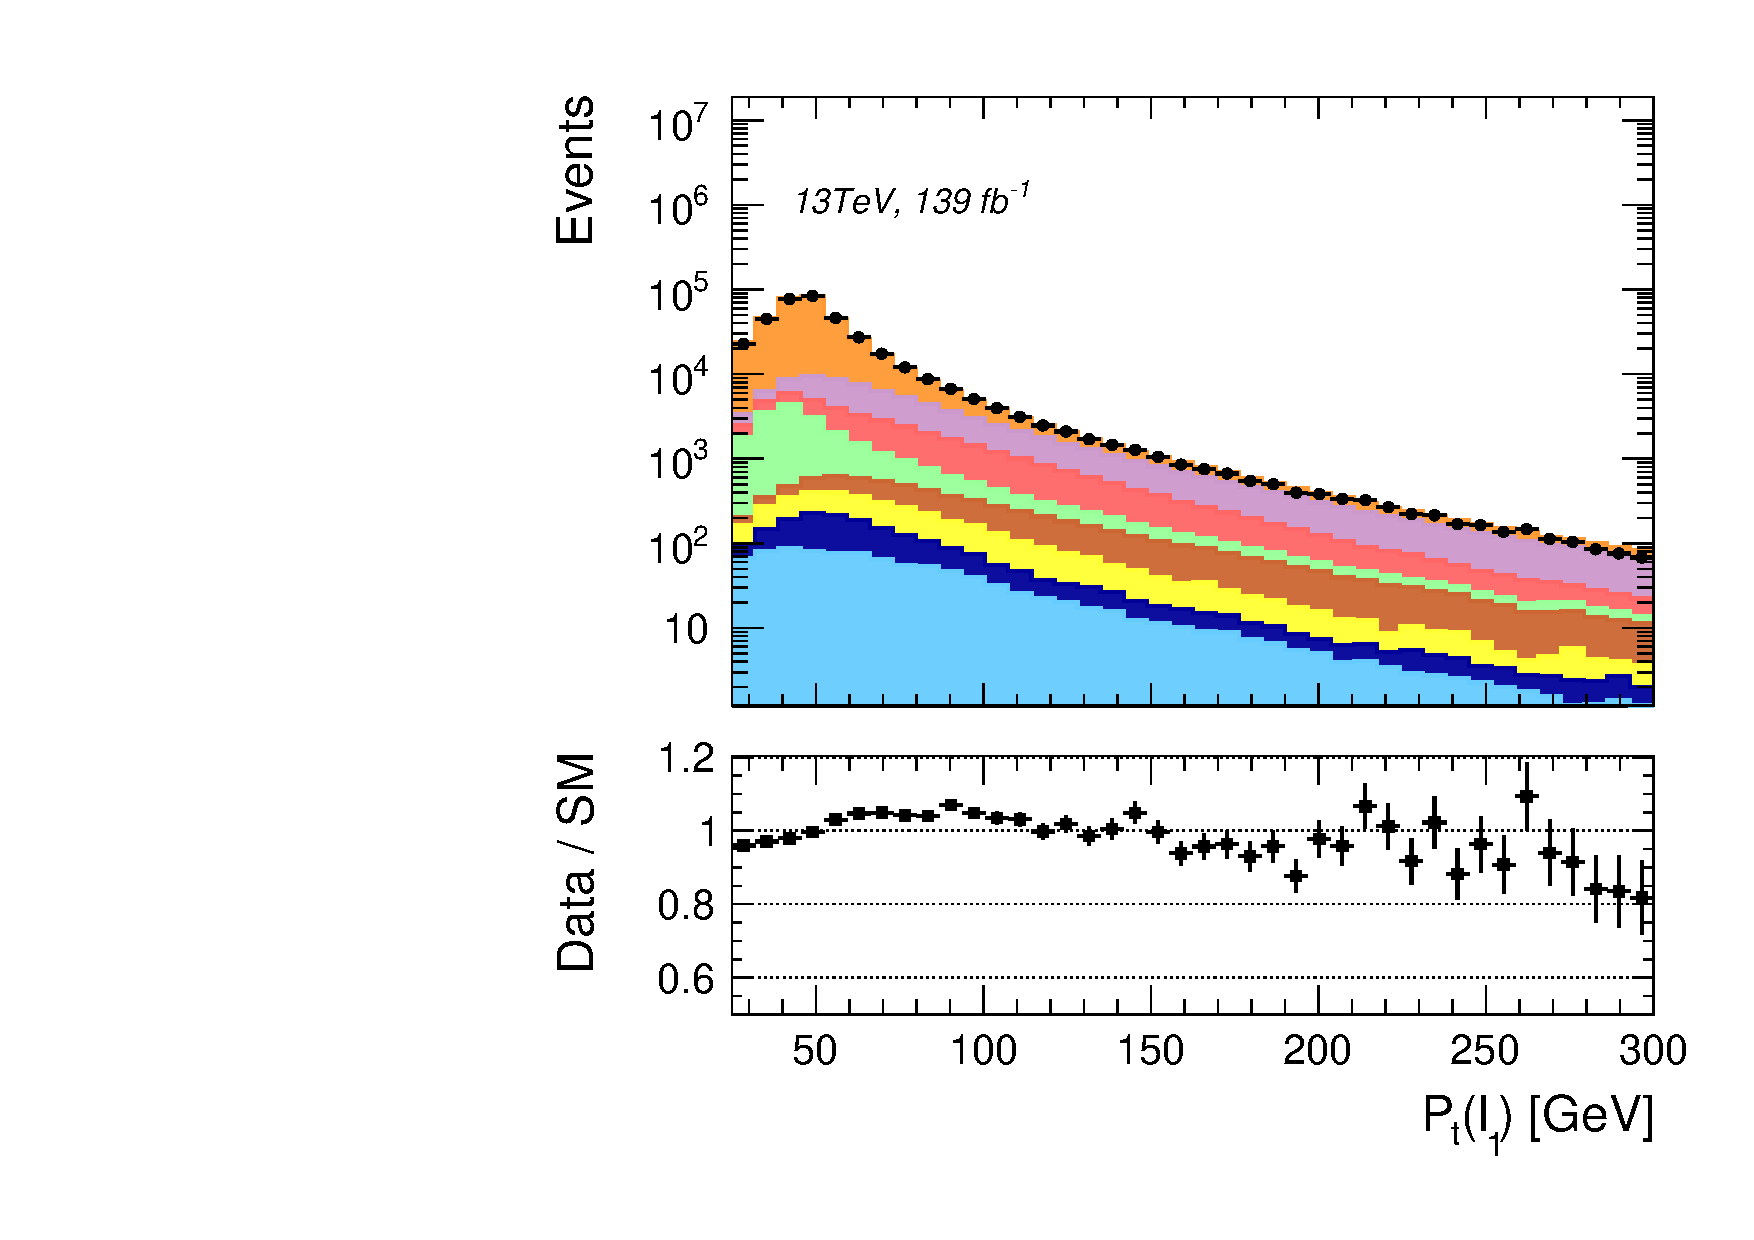
\includegraphics[width=\textwidth]{Figures/FeaturesHistograms/lep1_Pt.pdf}
        \caption{}
        \label{fig:lep1_Pt}
    \end{subfigure}
    \hfill
    \begin{subfigure}{.425\textwidth}
        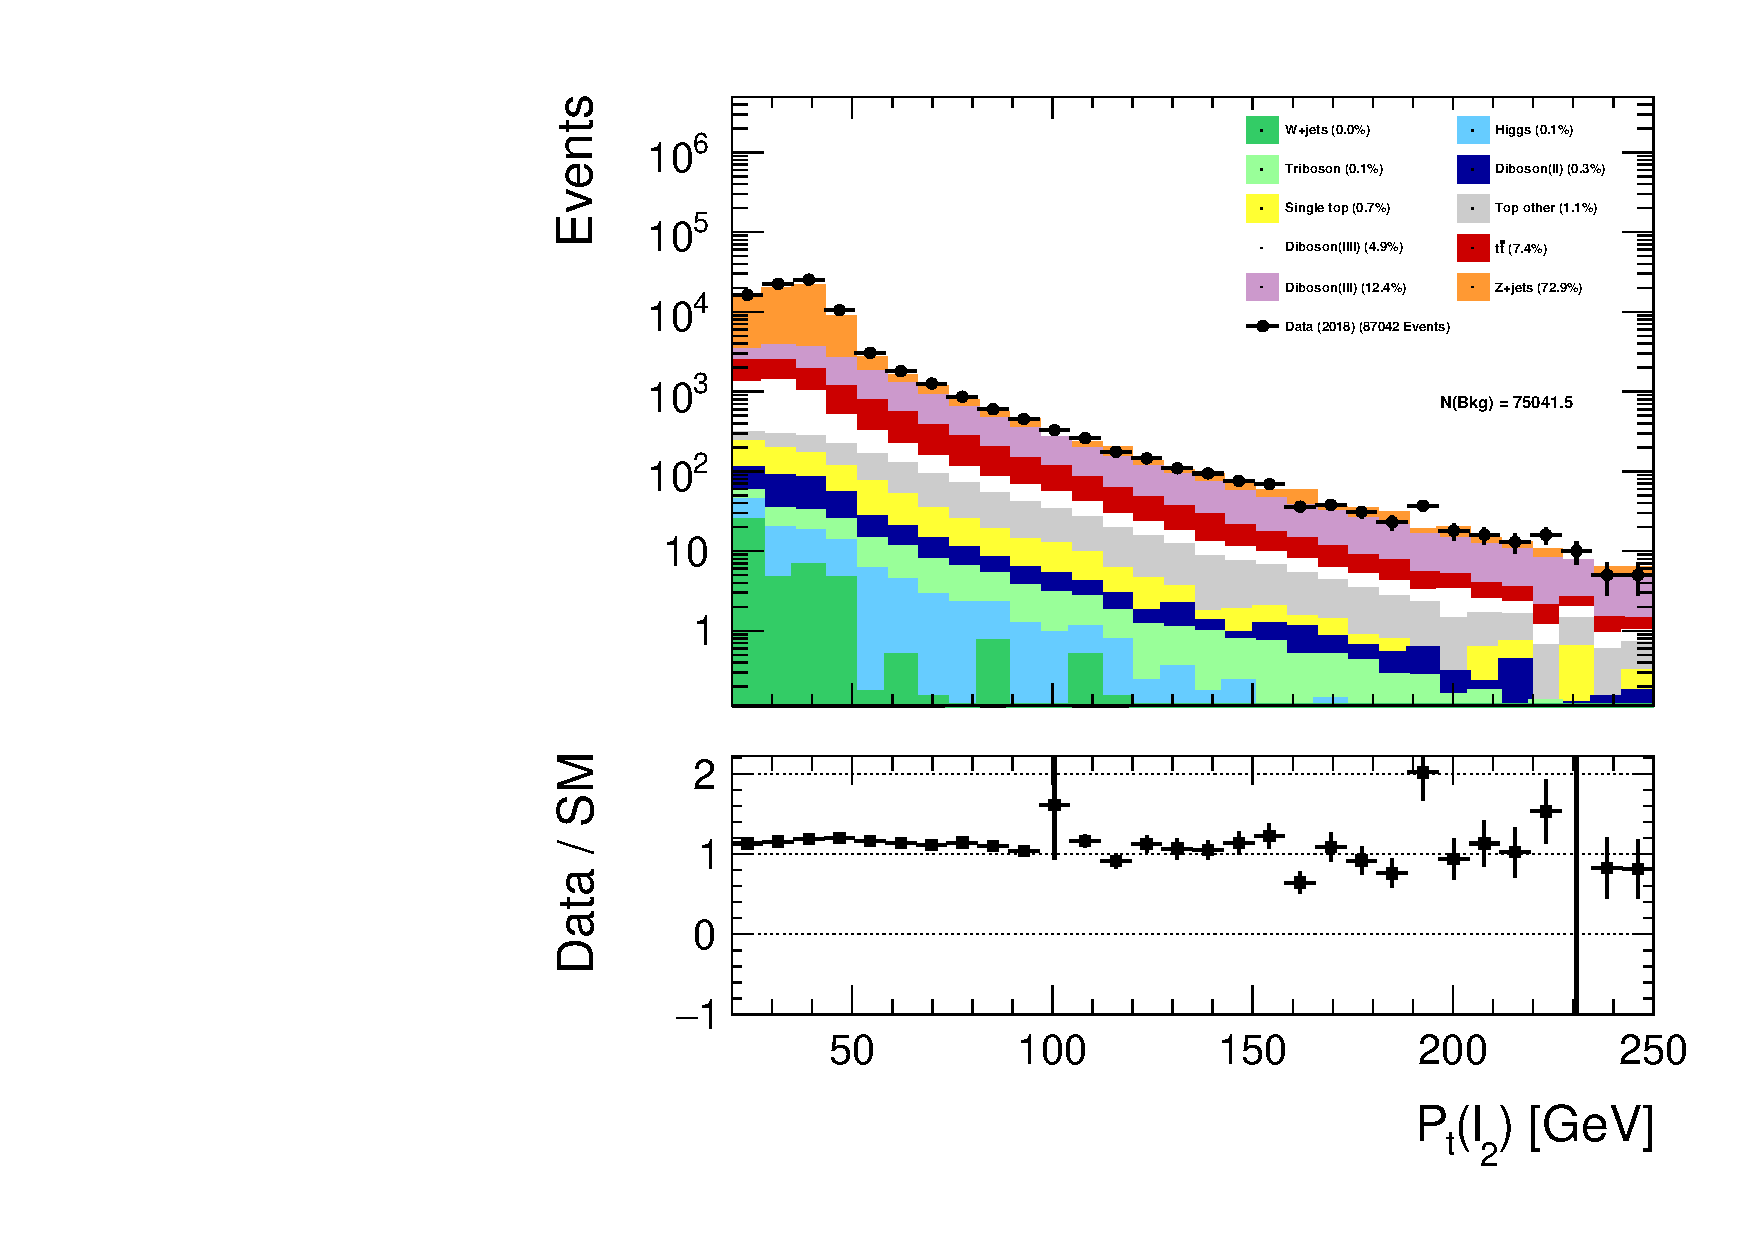
\includegraphics[width=\textwidth]{Figures/FeaturesHistograms/lep2_Pt.pdf}
        \caption{}
        \label{fig:lep2_Pt}
    \end{subfigure}
    }
    \makebox[0.9\linewidth][c]{%
    \begin{subfigure}{.425\textwidth}
        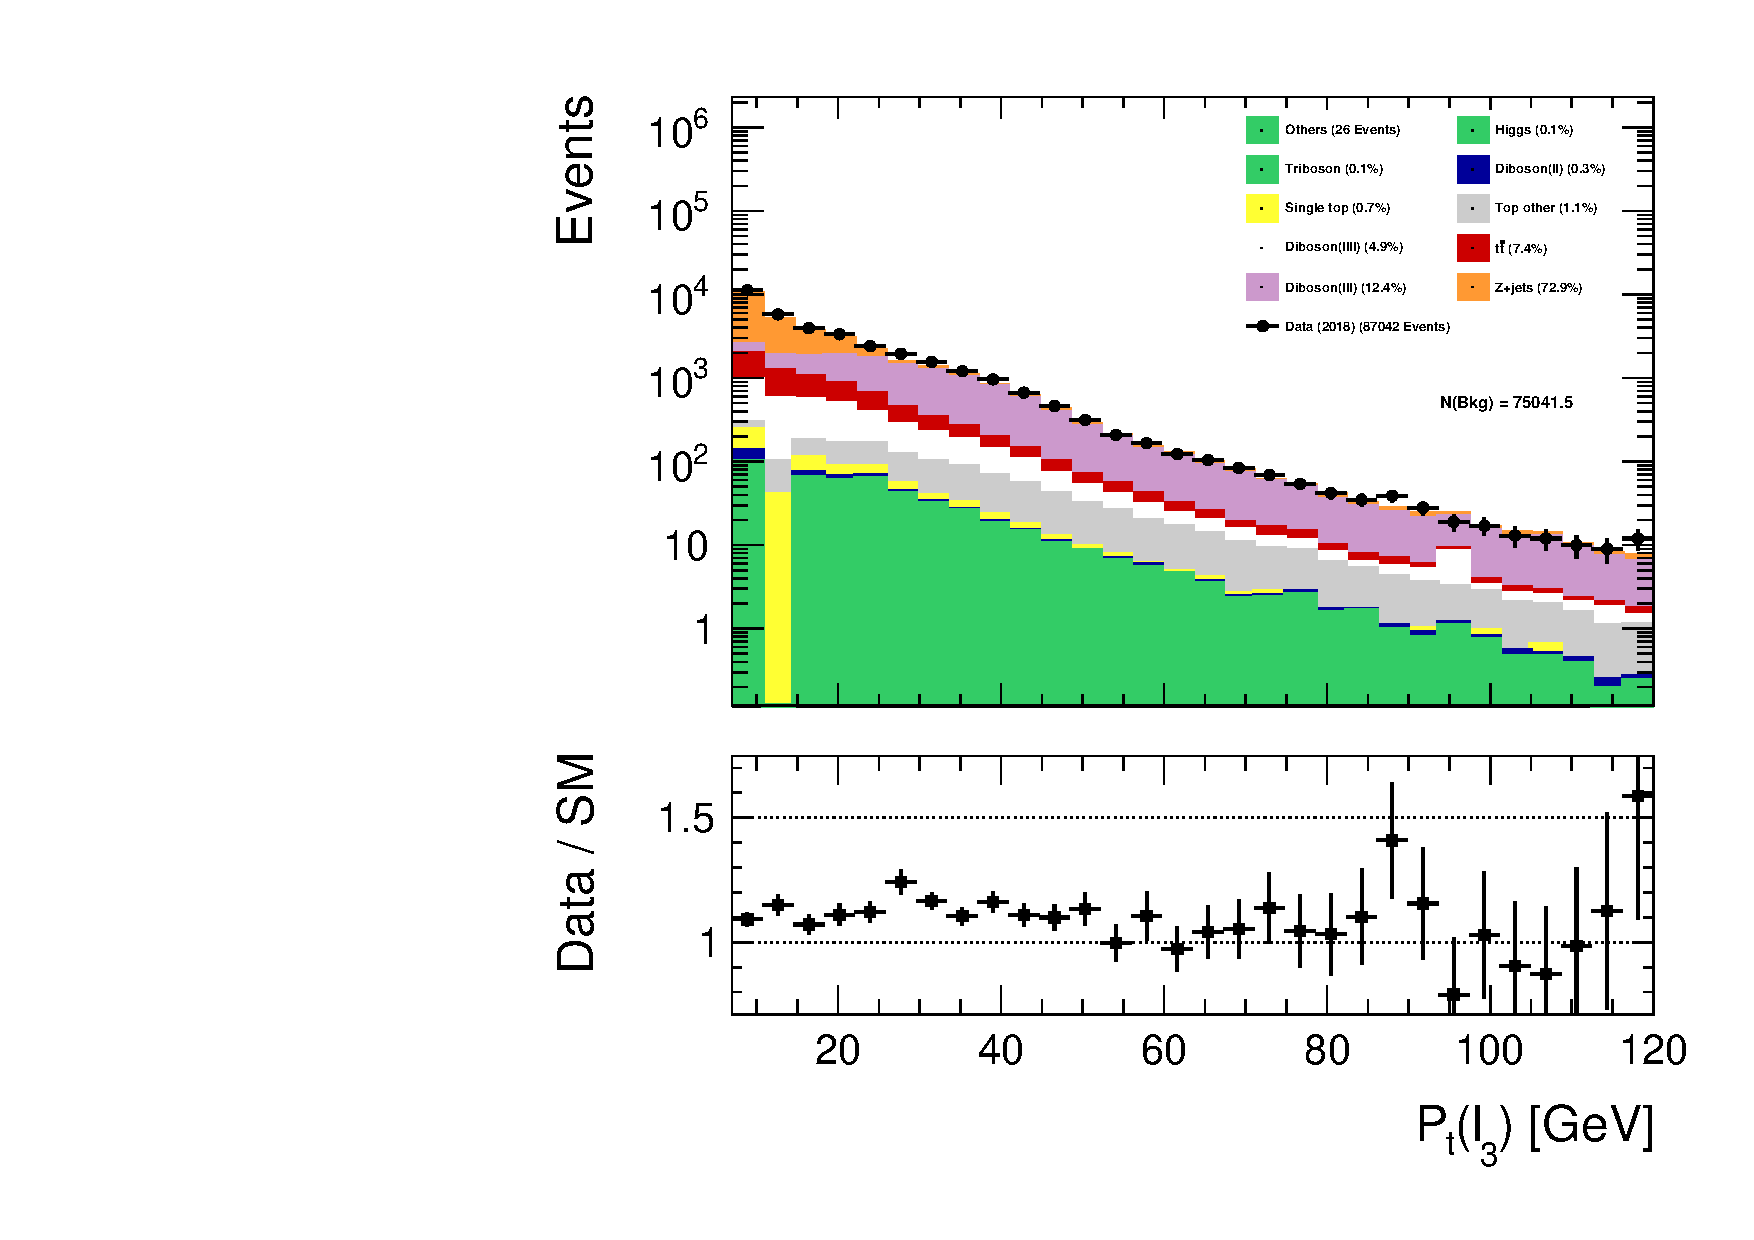
\includegraphics[width=\textwidth]{Figures/FeaturesHistograms/lep3_Pt.pdf}
        \caption{}
        \label{fig:lep3_Pt}
    \end{subfigure}
    \hfill
    \begin{subfigure}{.425\textwidth}
        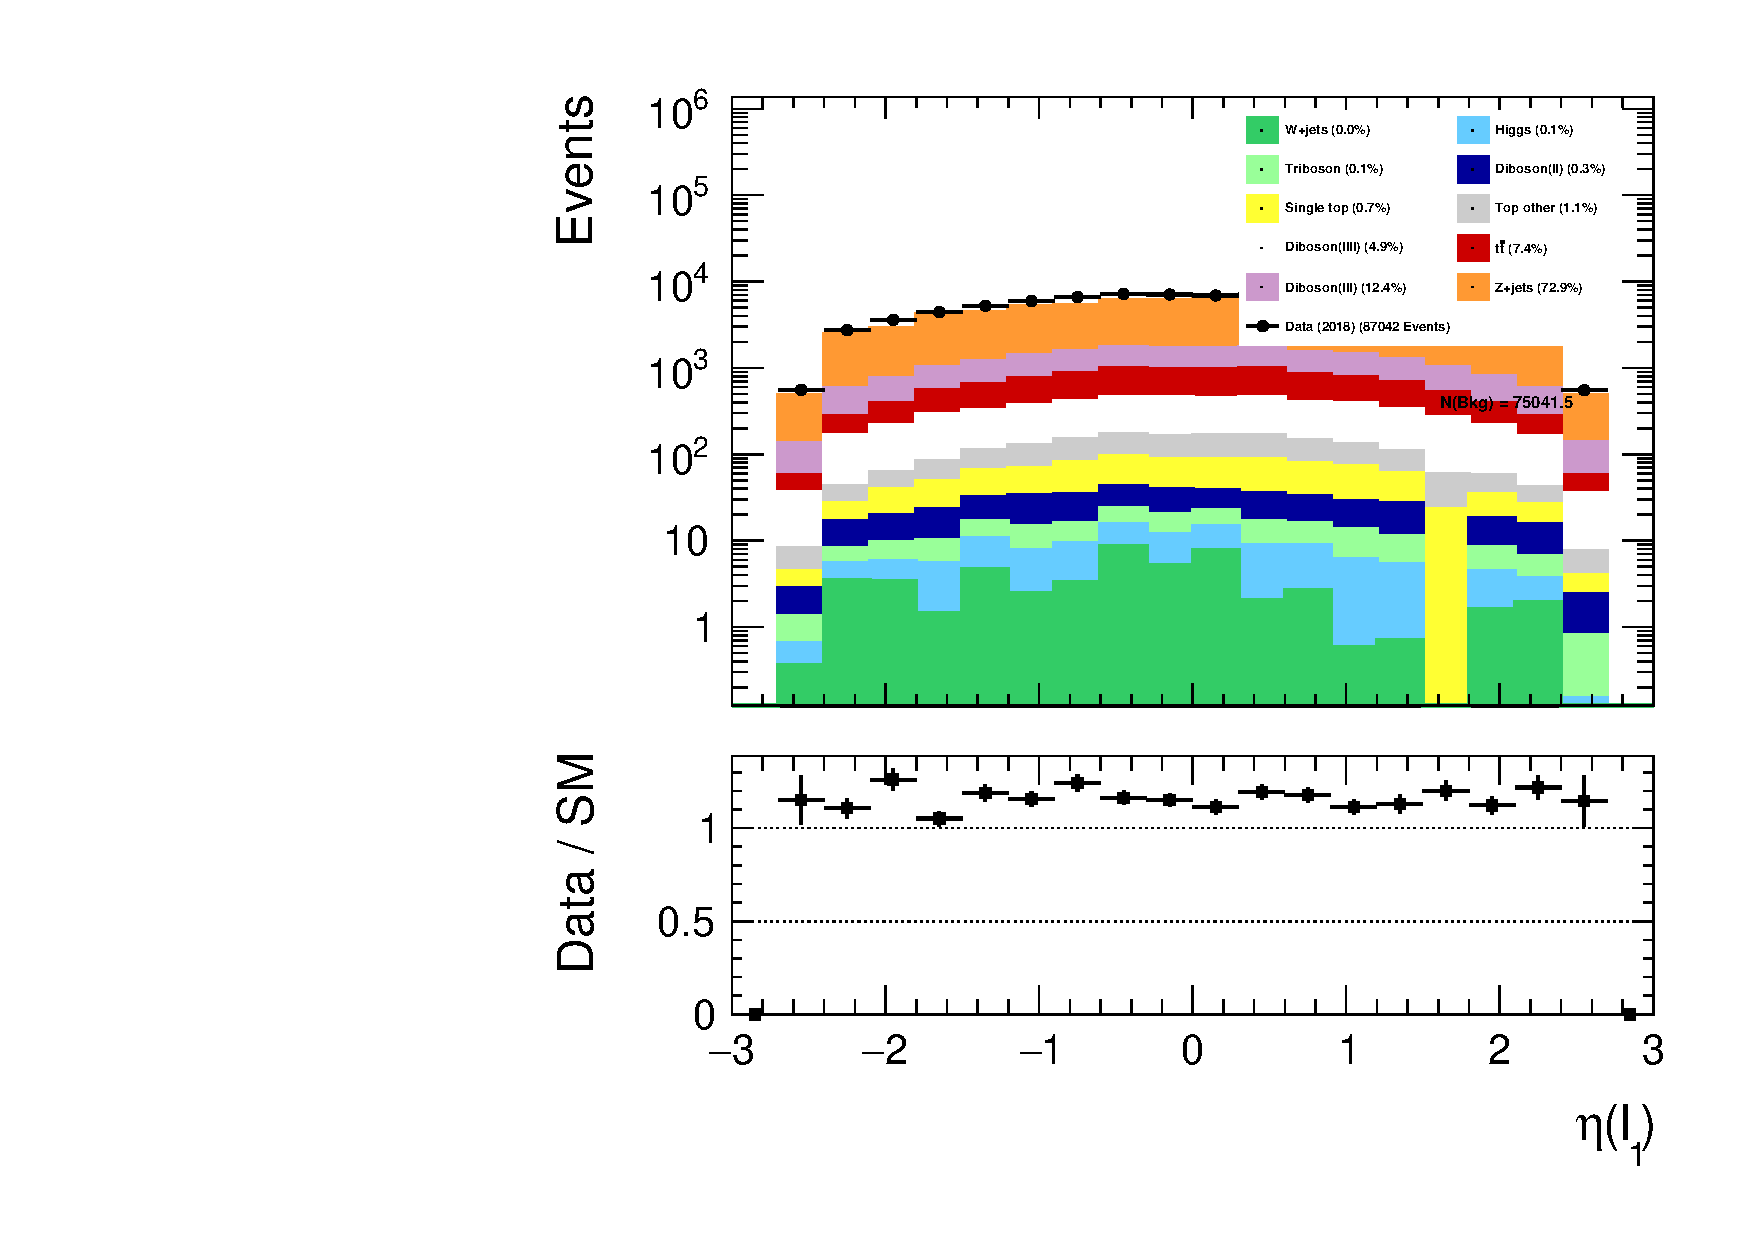
\includegraphics[width=\textwidth]{Figures/FeaturesHistograms/lep1_Eta.pdf}
        \caption{}
        \label{fig:lep1_Eta}
    \end{subfigure}
    }
    \makebox[0.9\linewidth][c]{%
    \begin{subfigure}{.425\textwidth}
        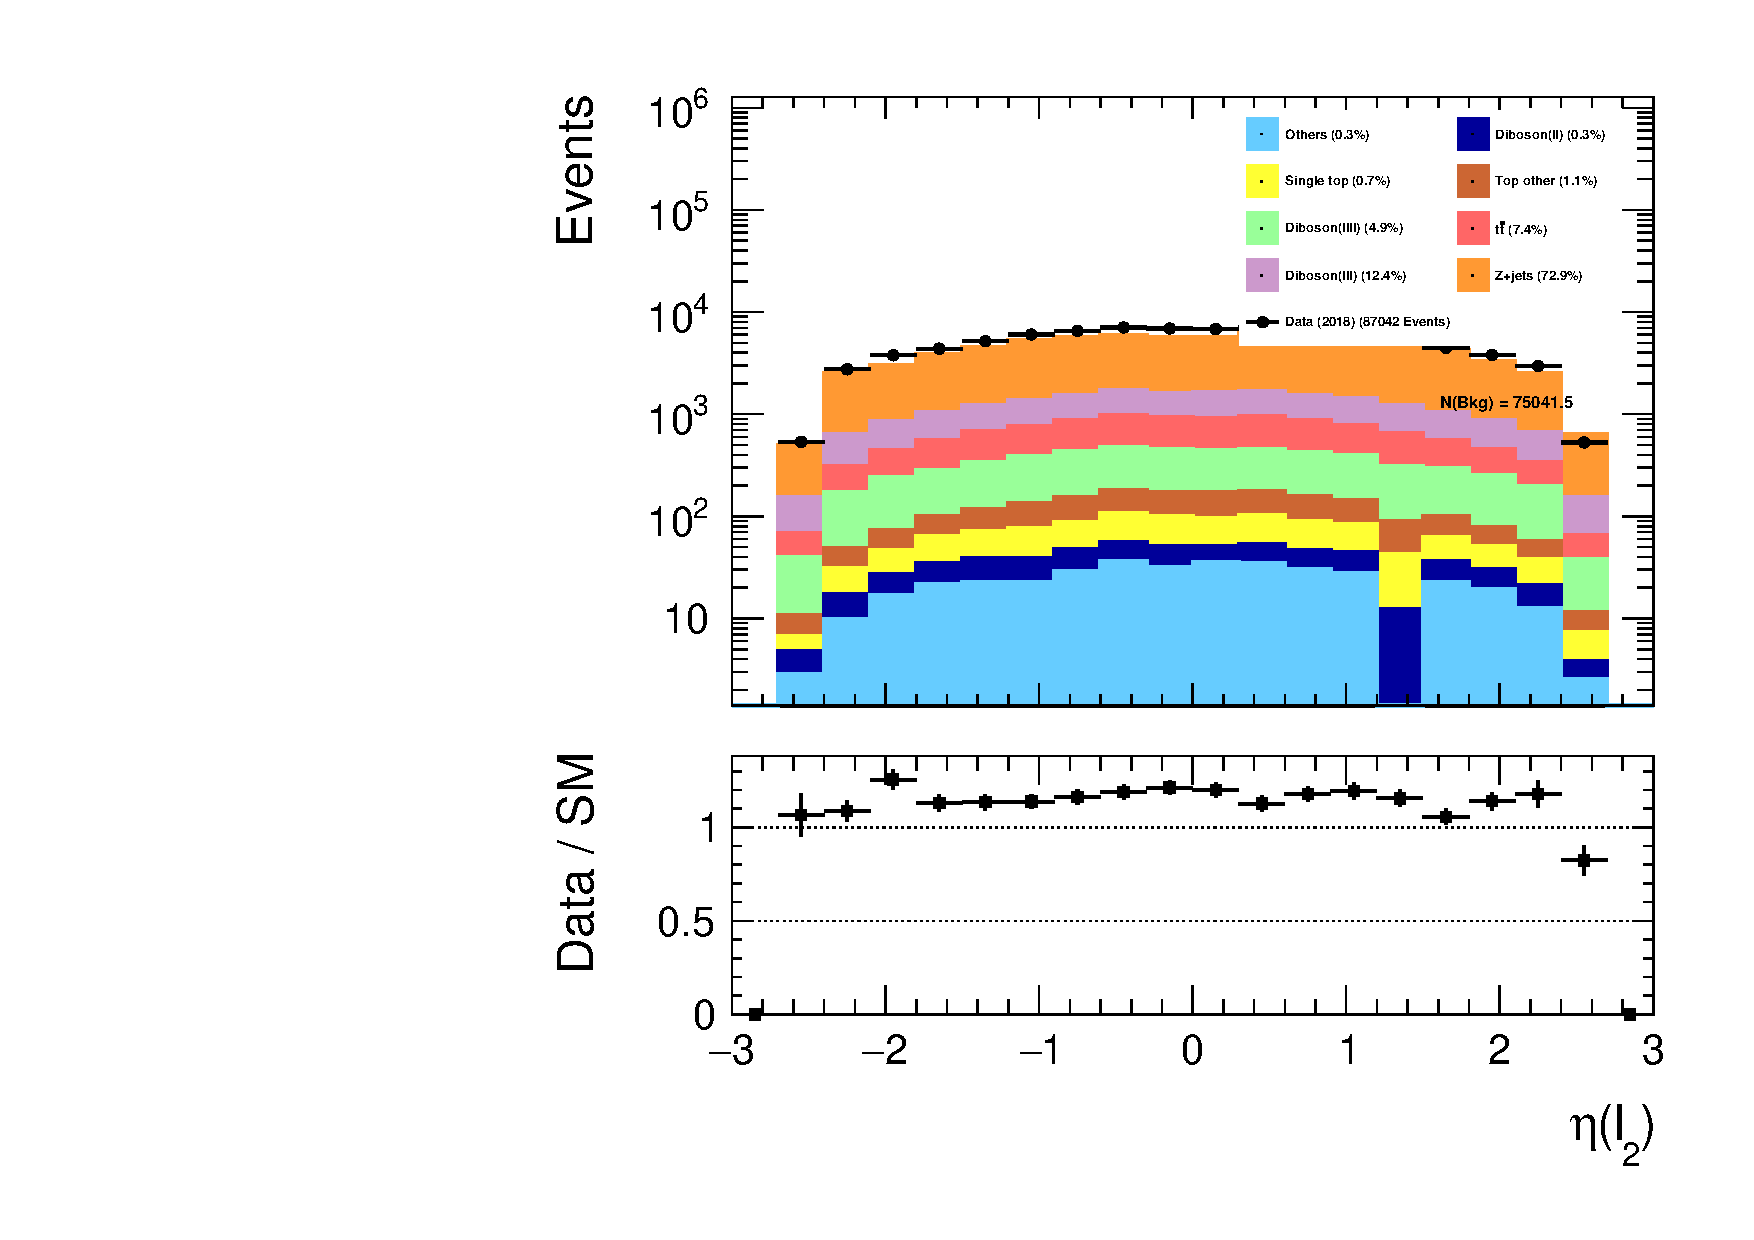
\includegraphics[width=\textwidth]{Figures/FeaturesHistograms/lep2_Eta.pdf}
        \caption{}
        \label{fig:lep2_Eta}
    \end{subfigure}
    \hfill
    \begin{subfigure}{.425\textwidth}
        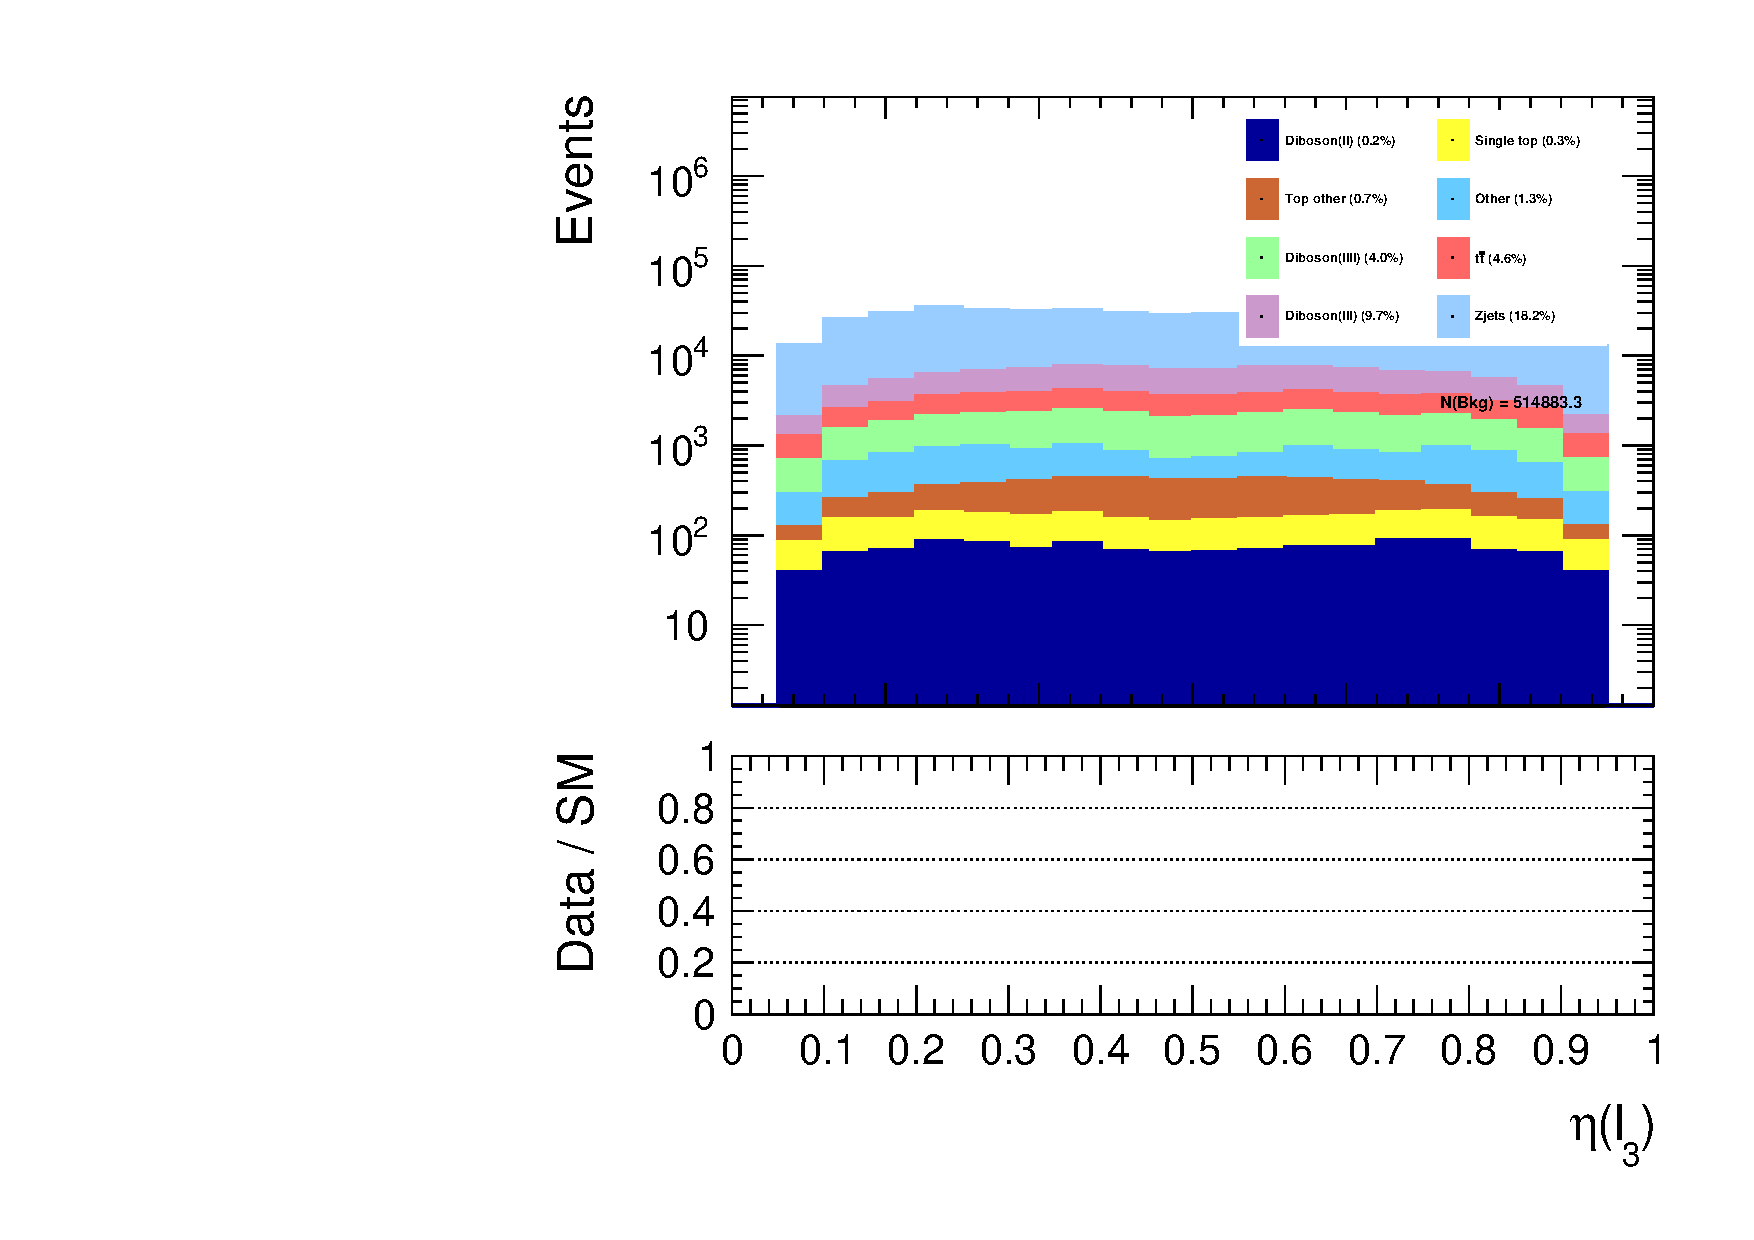
\includegraphics[width=\textwidth]{Figures/FeaturesHistograms/lep3_Eta.pdf}
        \caption{}
        \label{fig:lep3_Eta}
    \end{subfigure}
    }
    \caption{The event distribution for each channel over $P_t$ for the first \ref{fig:lep1_Pt}, 
    second \ref{fig:lep2_Pt} and third \ref{fig:lep3_Pt} lepton. Similarly, the distribution over $\eta$
    for the \ref{fig:lep1_Eta}, second \ref{fig:lep2_Eta} and third \ref{fig:lep3_Eta} lepton.}
    \label{fig:Dist1}
\end{figure}
\newpage
\begin{figure}
    \makebox[0.9\linewidth][c]{%
    \centering
    \begin{subfigure}{.425\textwidth}
        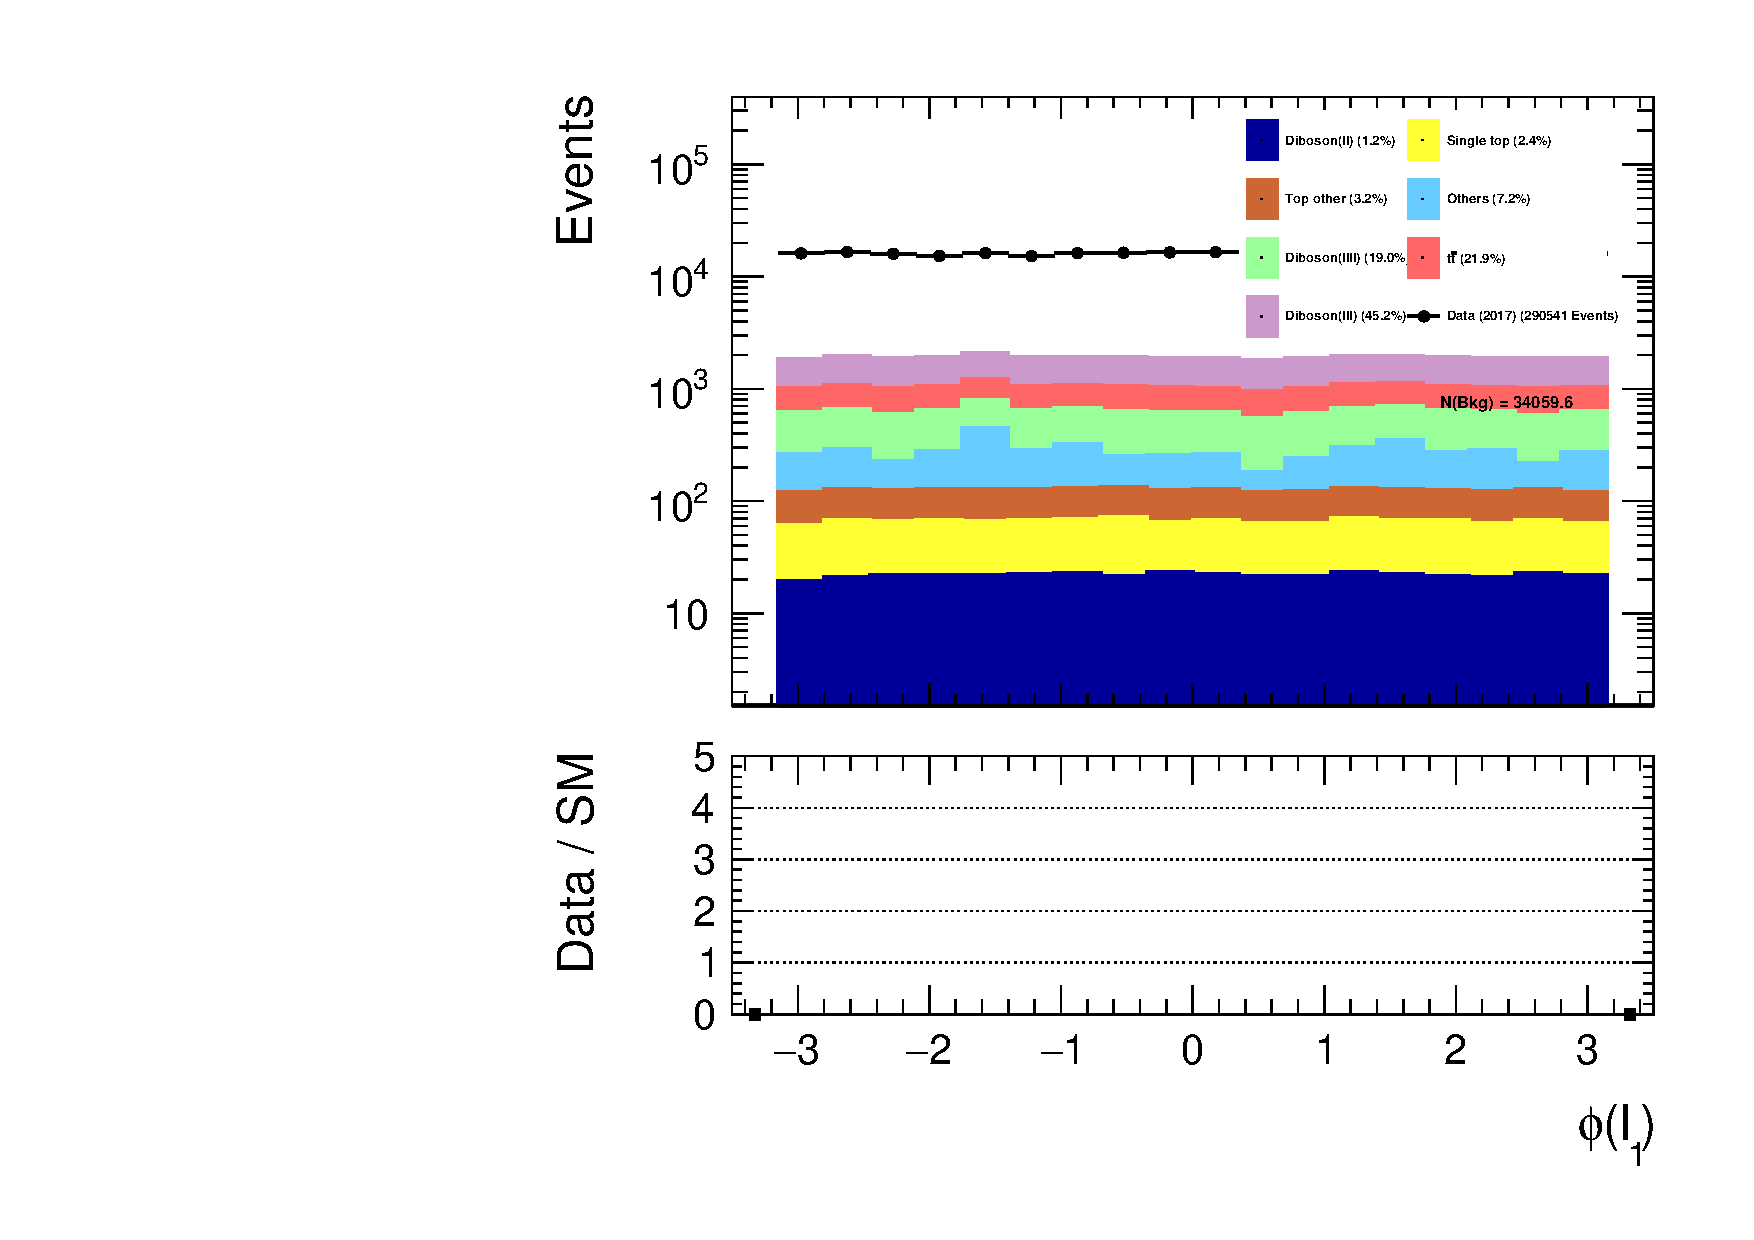
\includegraphics[width=\textwidth]{Figures/FeaturesHistograms/lep1_Phi.pdf}
        \caption{}
        \label{fig:lep1_Phi}
    \end{subfigure}
    \hfill
    \begin{subfigure}{.425\textwidth}
        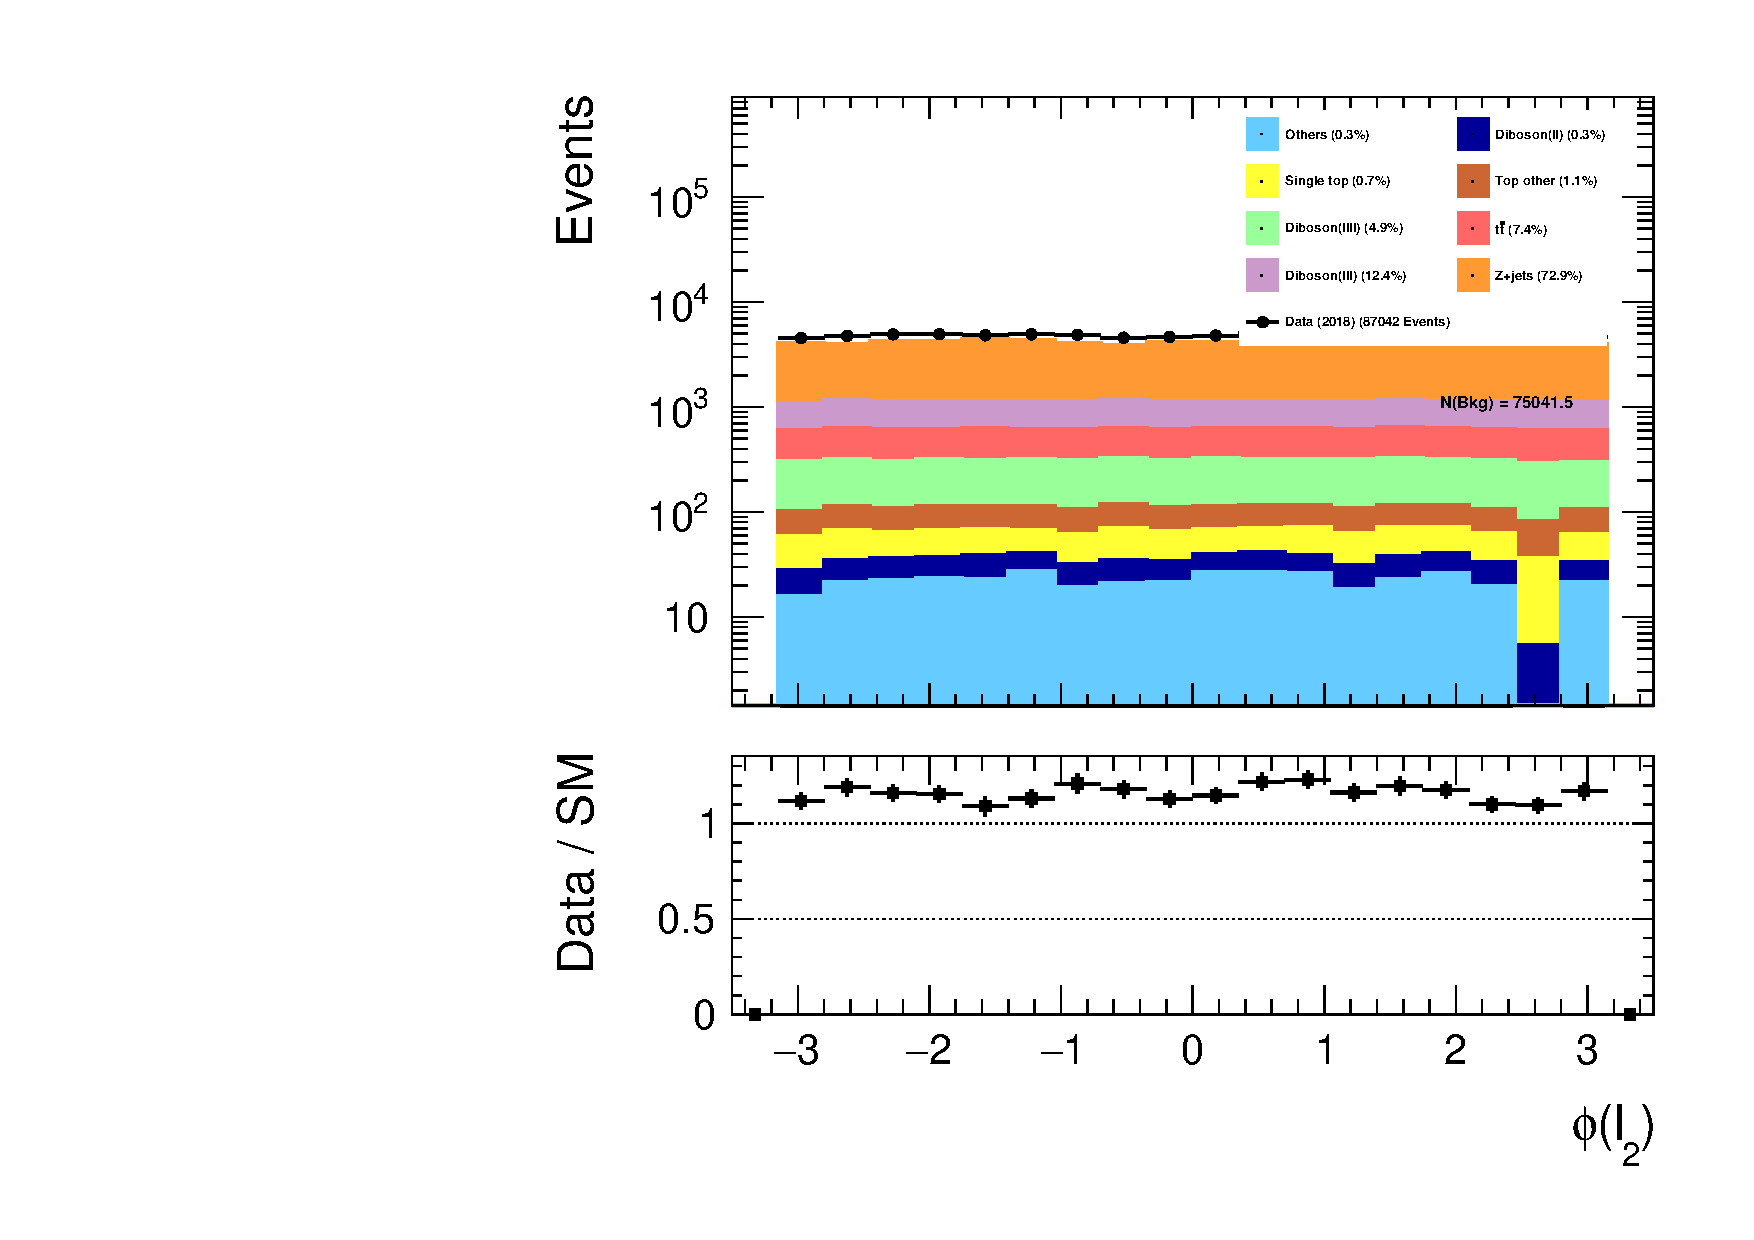
\includegraphics[width=\textwidth]{Figures/FeaturesHistograms/lep2_Phi.pdf}
        \caption{}
        \label{fig:lep2_Phi}
    \end{subfigure}
    }
    \makebox[0.9\linewidth][c]{%
    \begin{subfigure}{.425\textwidth}
        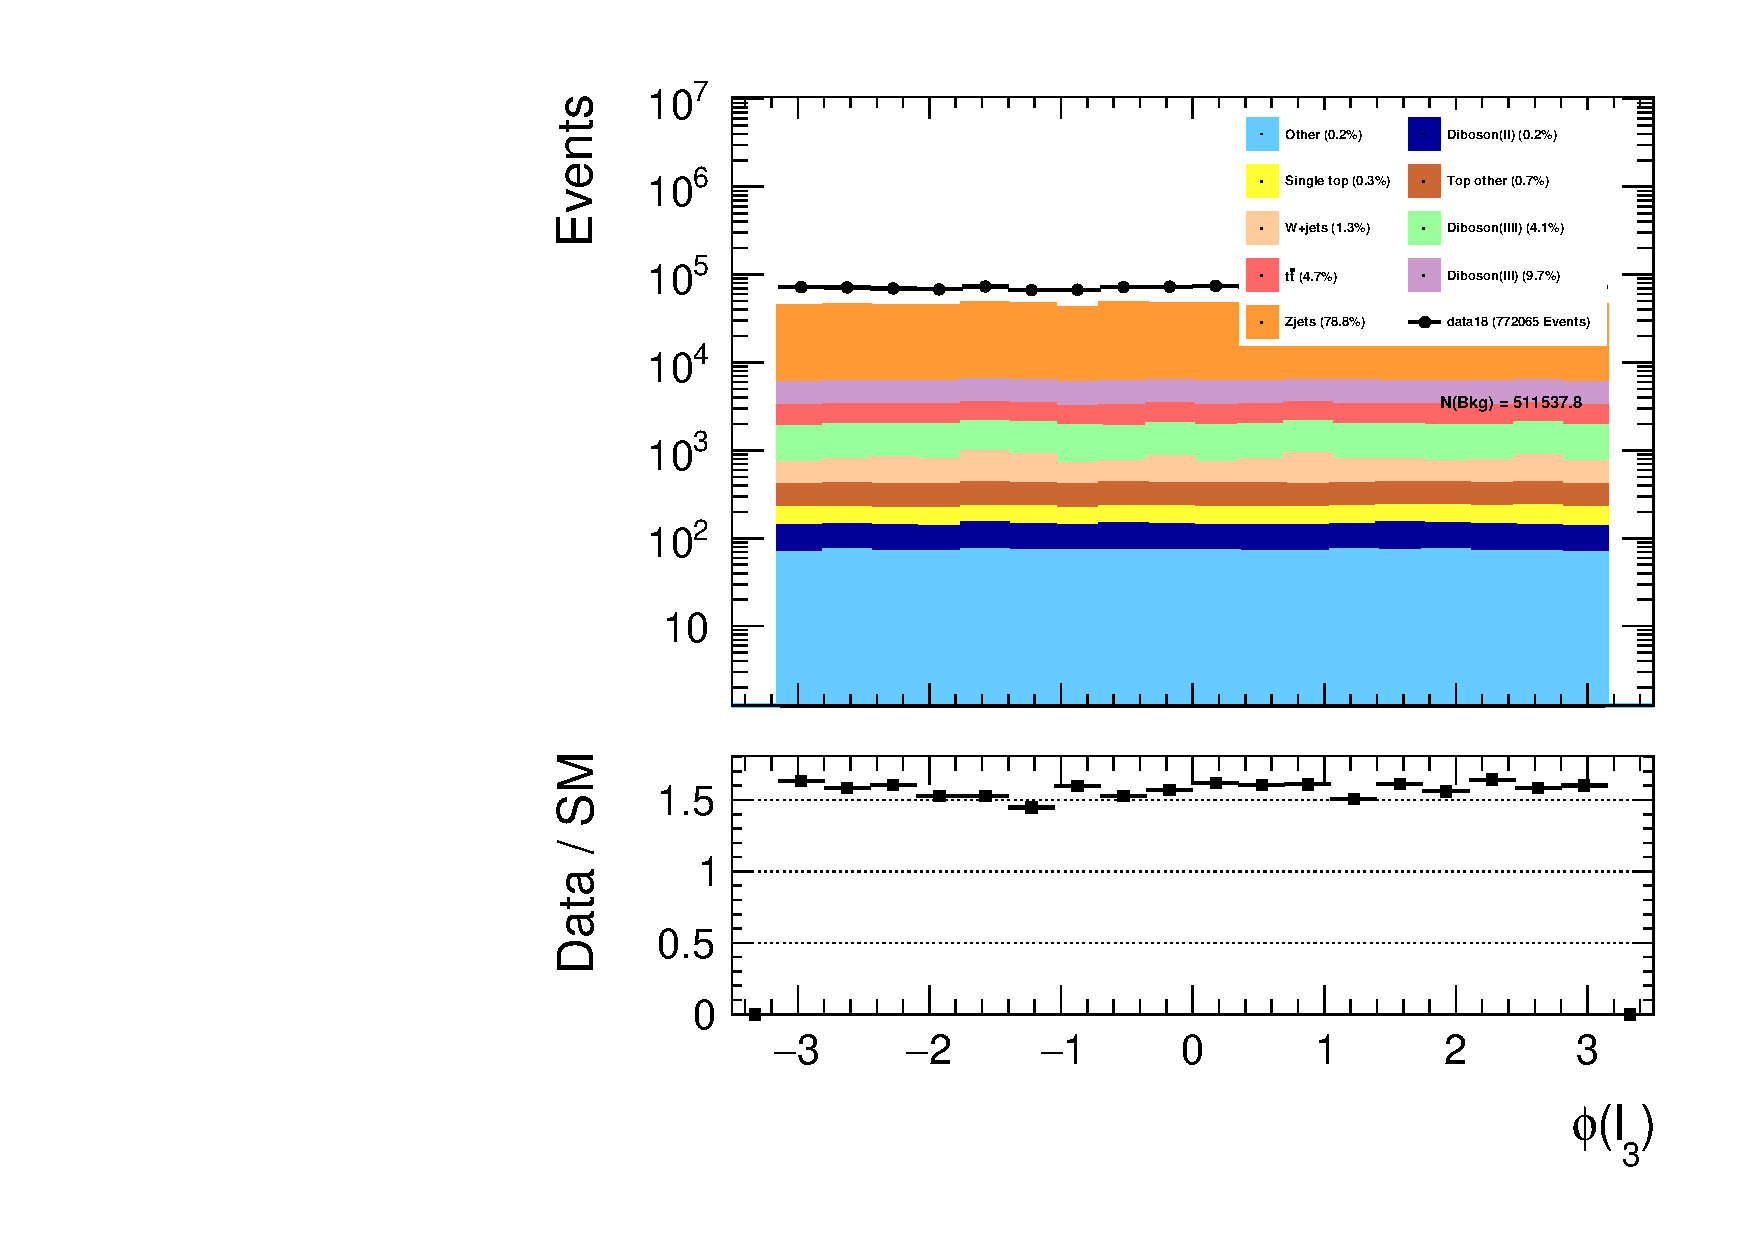
\includegraphics[width=\textwidth]{Figures/FeaturesHistograms/lep3_Phi.pdf}
        \caption{}
        \label{fig:lep3_Phi}
    \end{subfigure}
    \hfill
    \begin{subfigure}{.425\textwidth}
        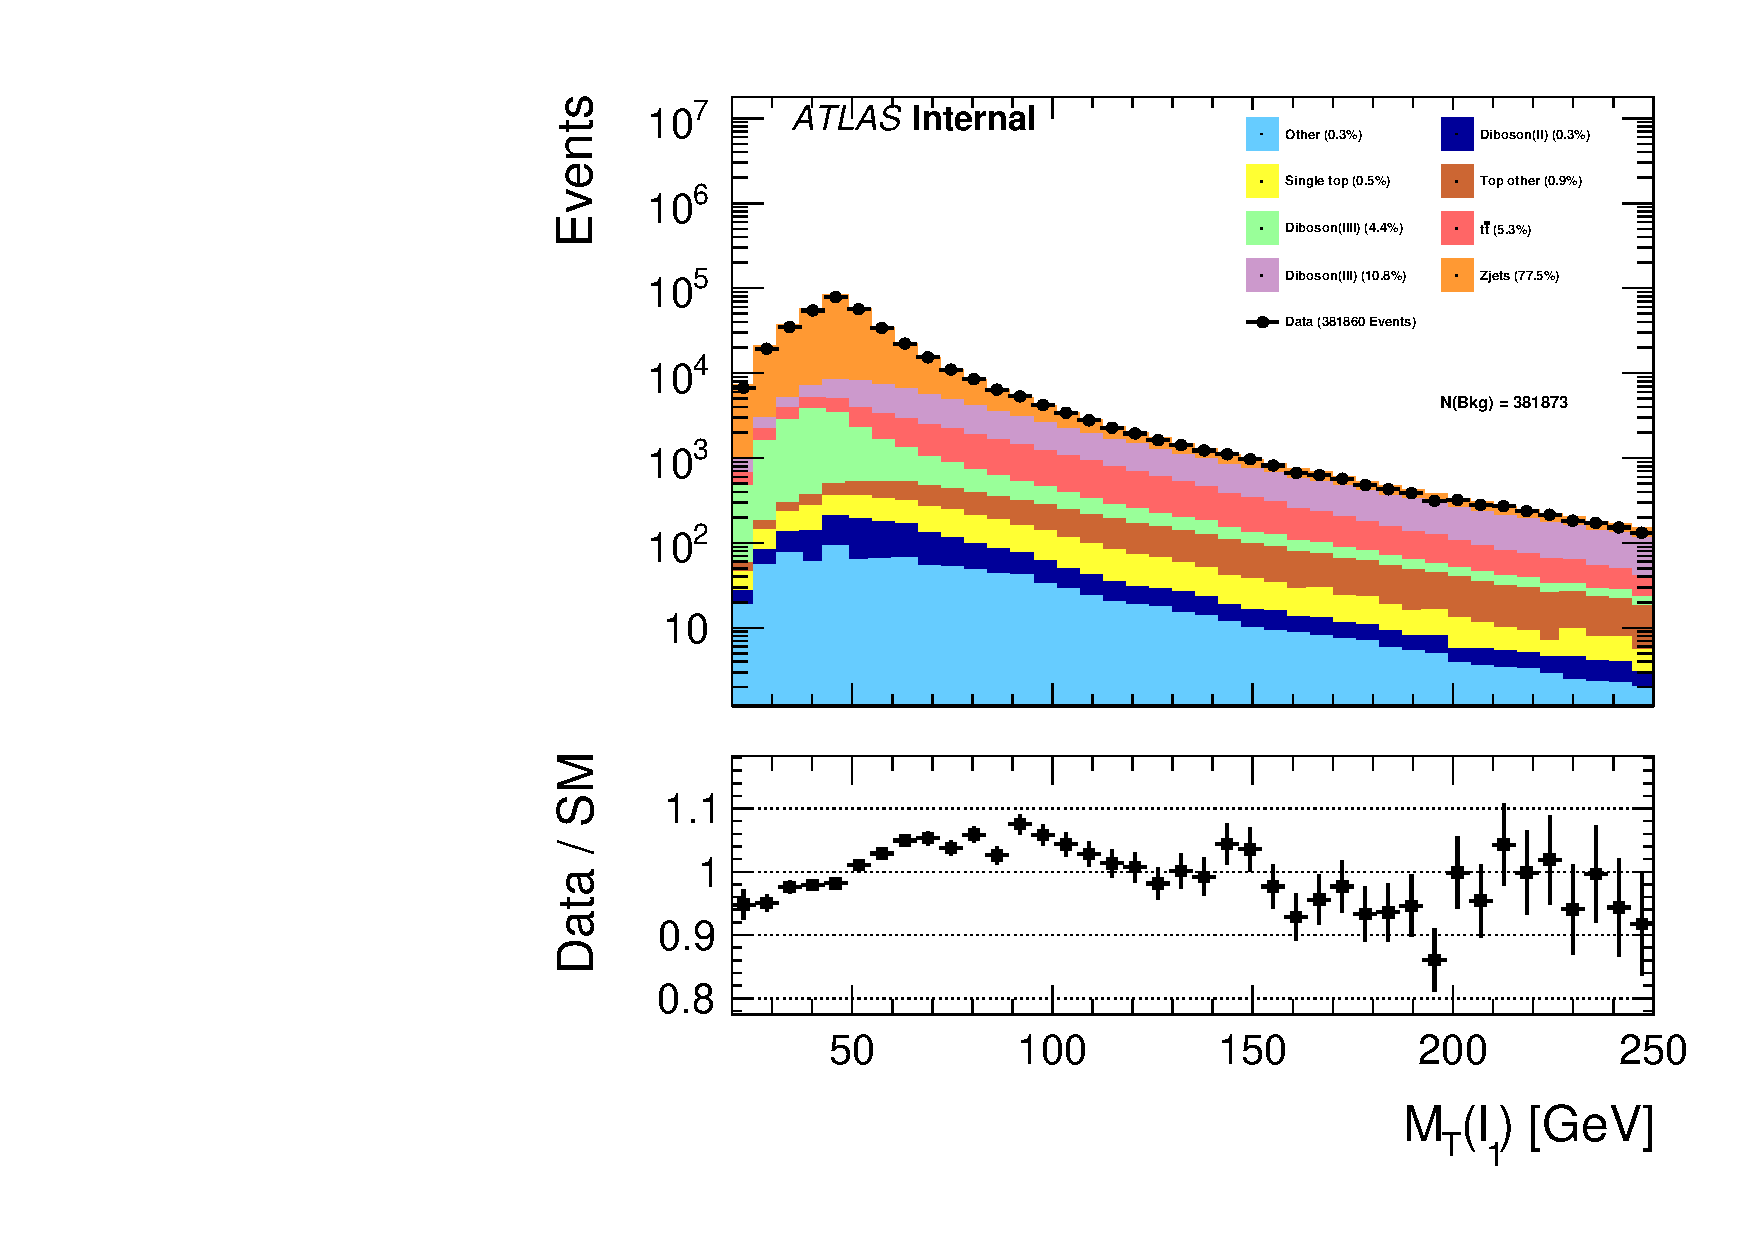
\includegraphics[width=\textwidth]{Figures/FeaturesHistograms/lep1_Mt.pdf}
        \caption{}
        \label{fig:lep1_Mt}
    \end{subfigure}
    }
    \makebox[0.9\linewidth][c]{%
    \begin{subfigure}{.425\textwidth}
        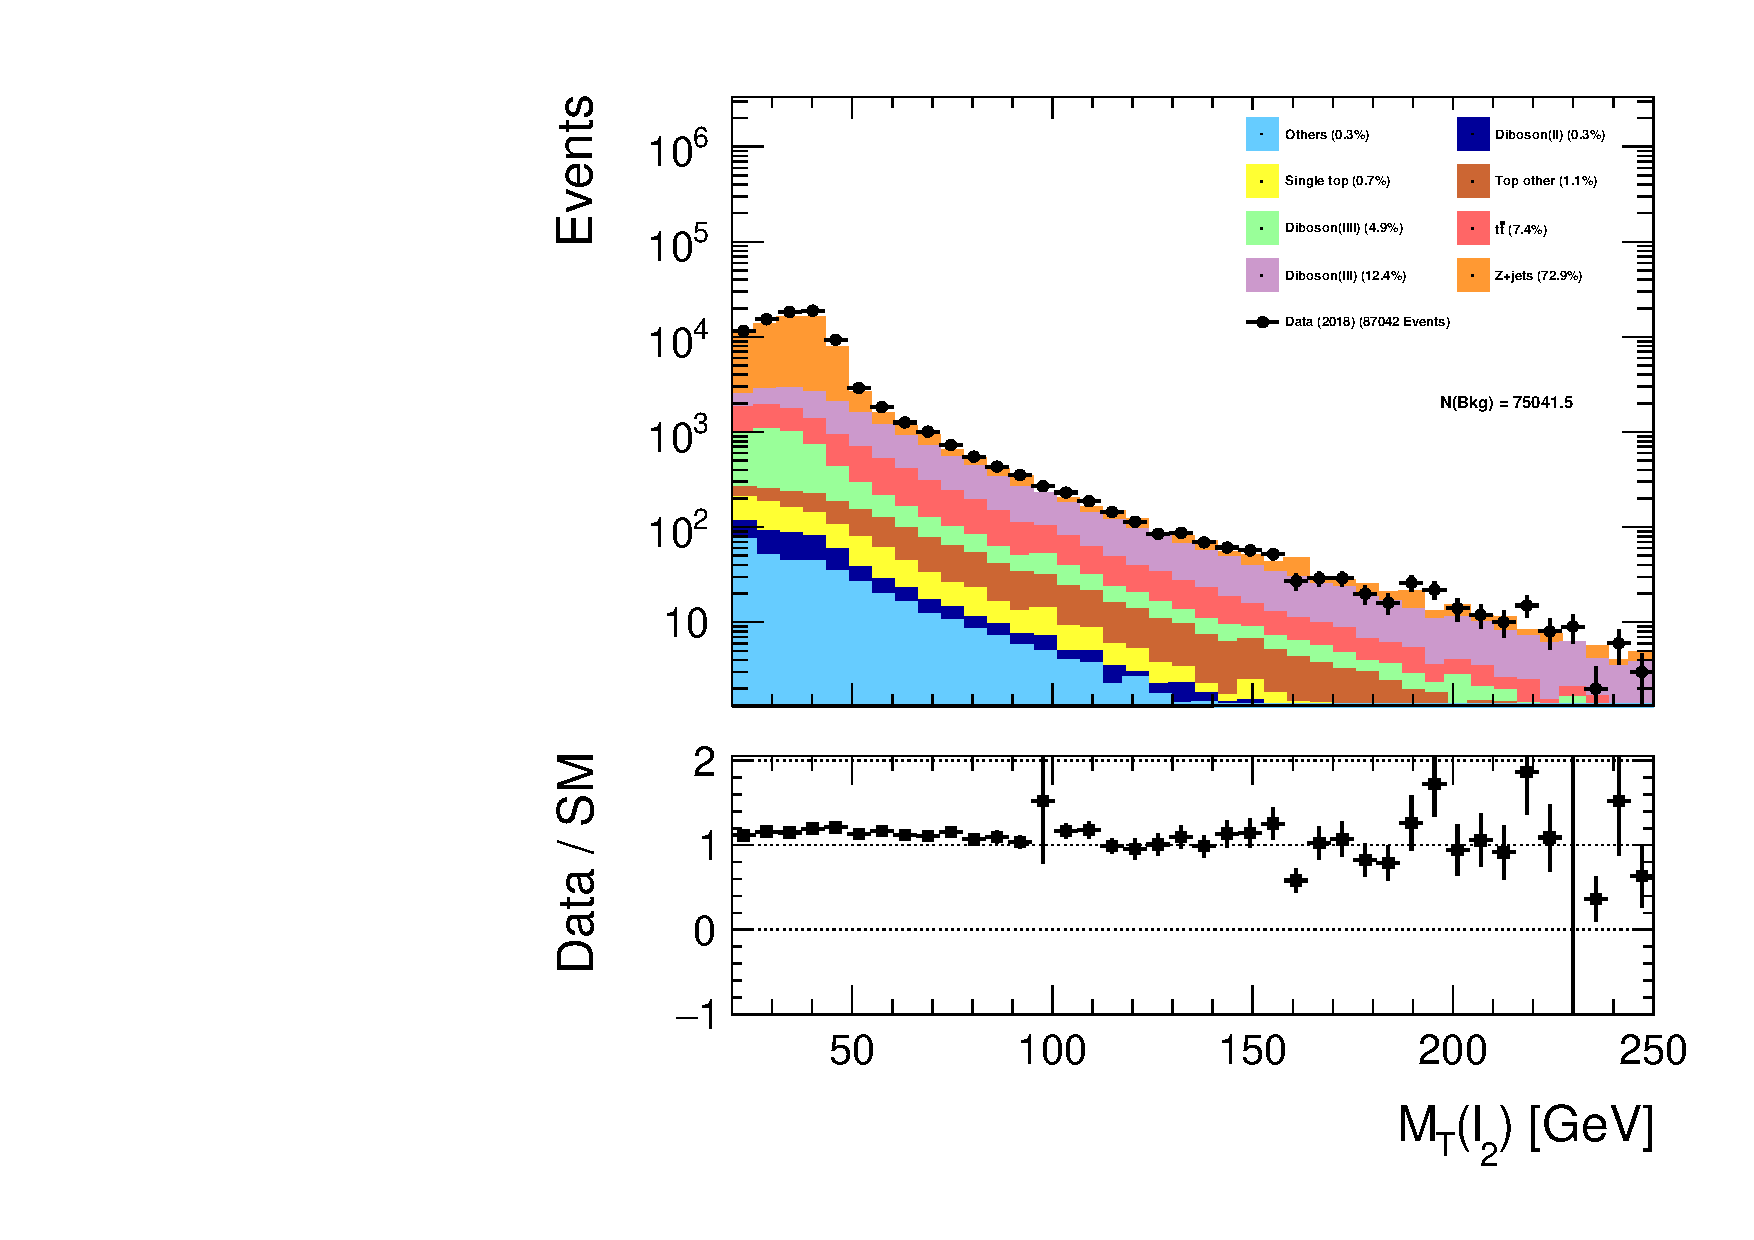
\includegraphics[width=\textwidth]{Figures/FeaturesHistograms/lep2_Mt.pdf}
        \caption{}
        \label{fig:lep2_Mt}
    \end{subfigure}
    \hfill
    \begin{subfigure}{.425\textwidth}
        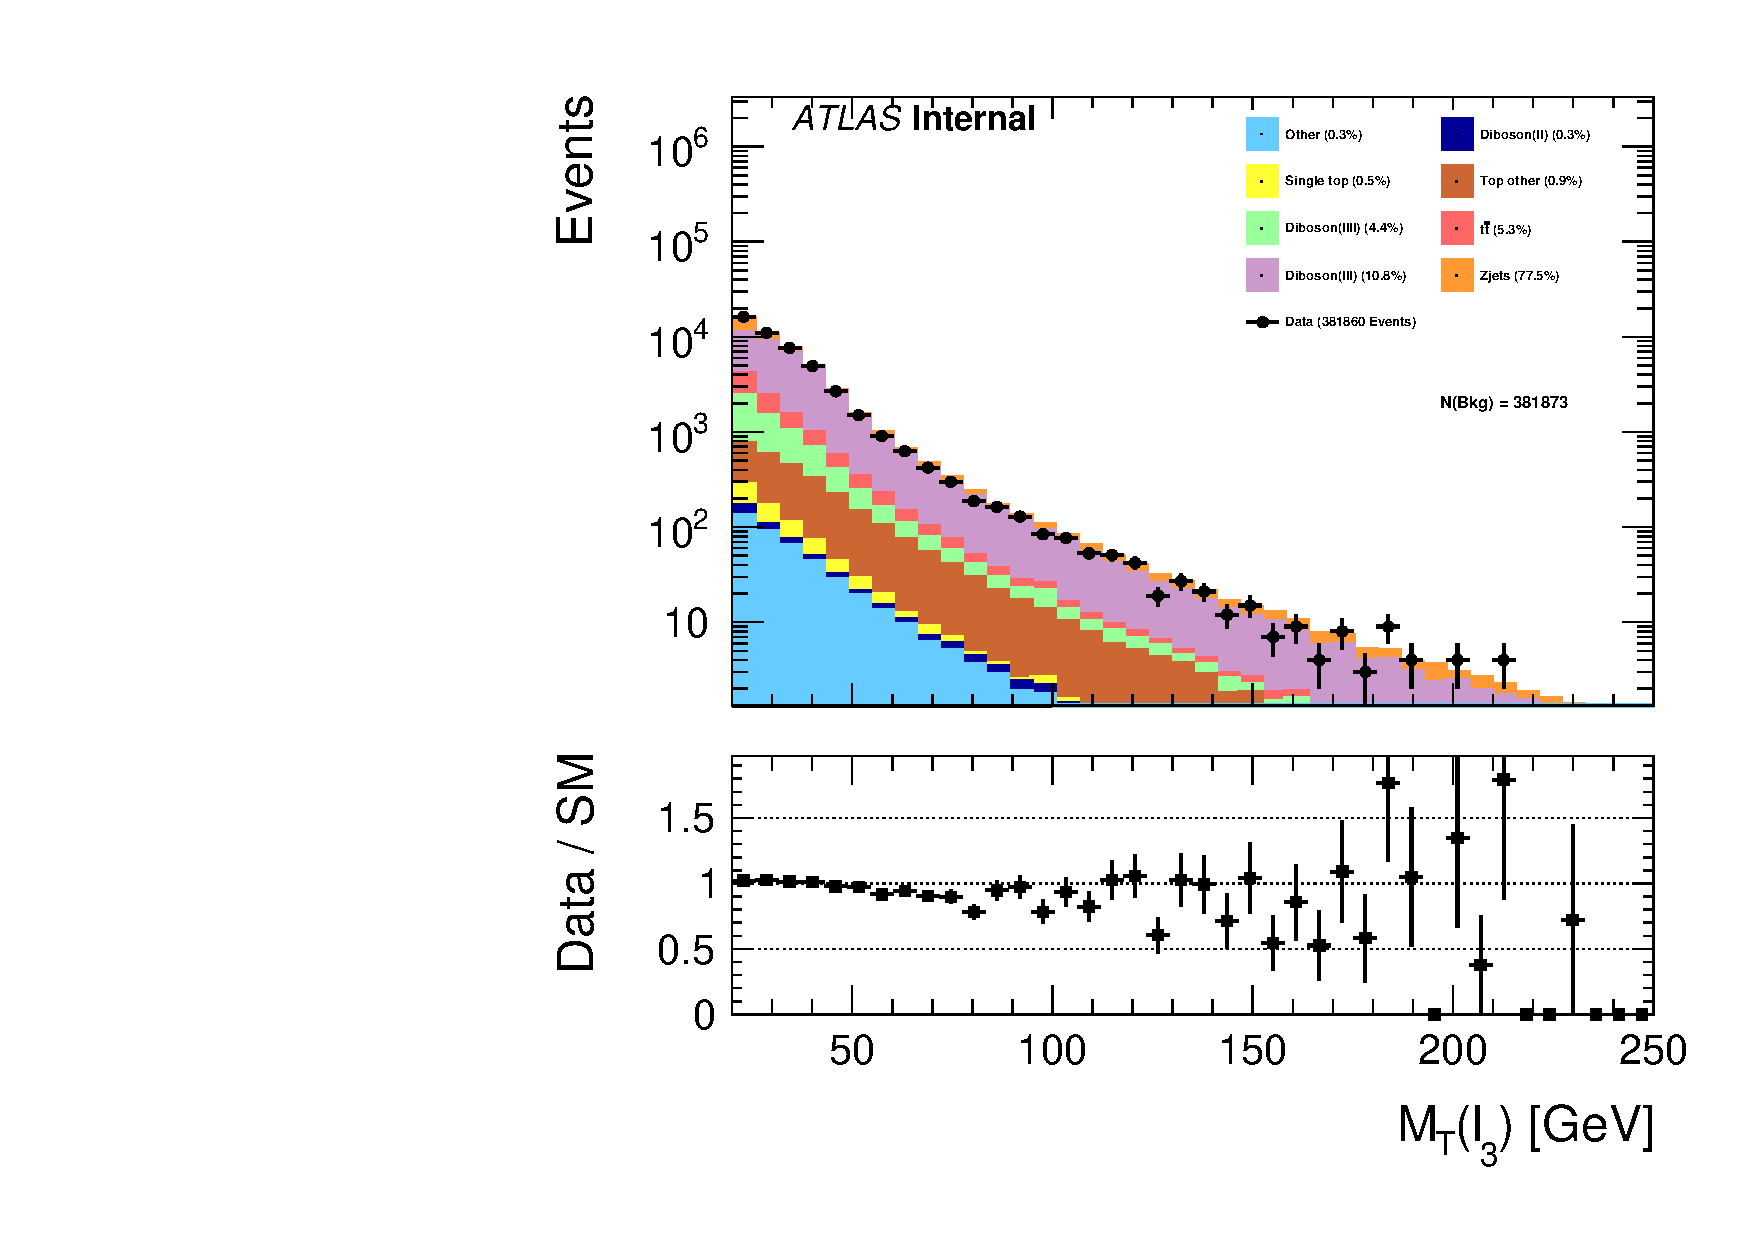
\includegraphics[width=\textwidth]{Figures/FeaturesHistograms/lep3_Mt.pdf}
        \caption{}
        \label{fig:lep3_Mt}
    \end{subfigure}
    }
    \caption{The event distribution for each channel over $\phi$ for the first \ref{fig:lep1_Phi}, 
    second \ref{fig:lep2_Phi} and third \ref{fig:lep3_Phi} lepton. Similarly, the distribution over $m_t$
    for the first \ref{fig:lep1_Mt}, second \ref{fig:lep2_Mt} and third \ref{fig:lep3_Mt} lepton.}
\end{figure}
\newpage
\begin{figure}
    \makebox[0.9\linewidth][c]{%
    \centering
    \begin{subfigure}{.425\textwidth}
        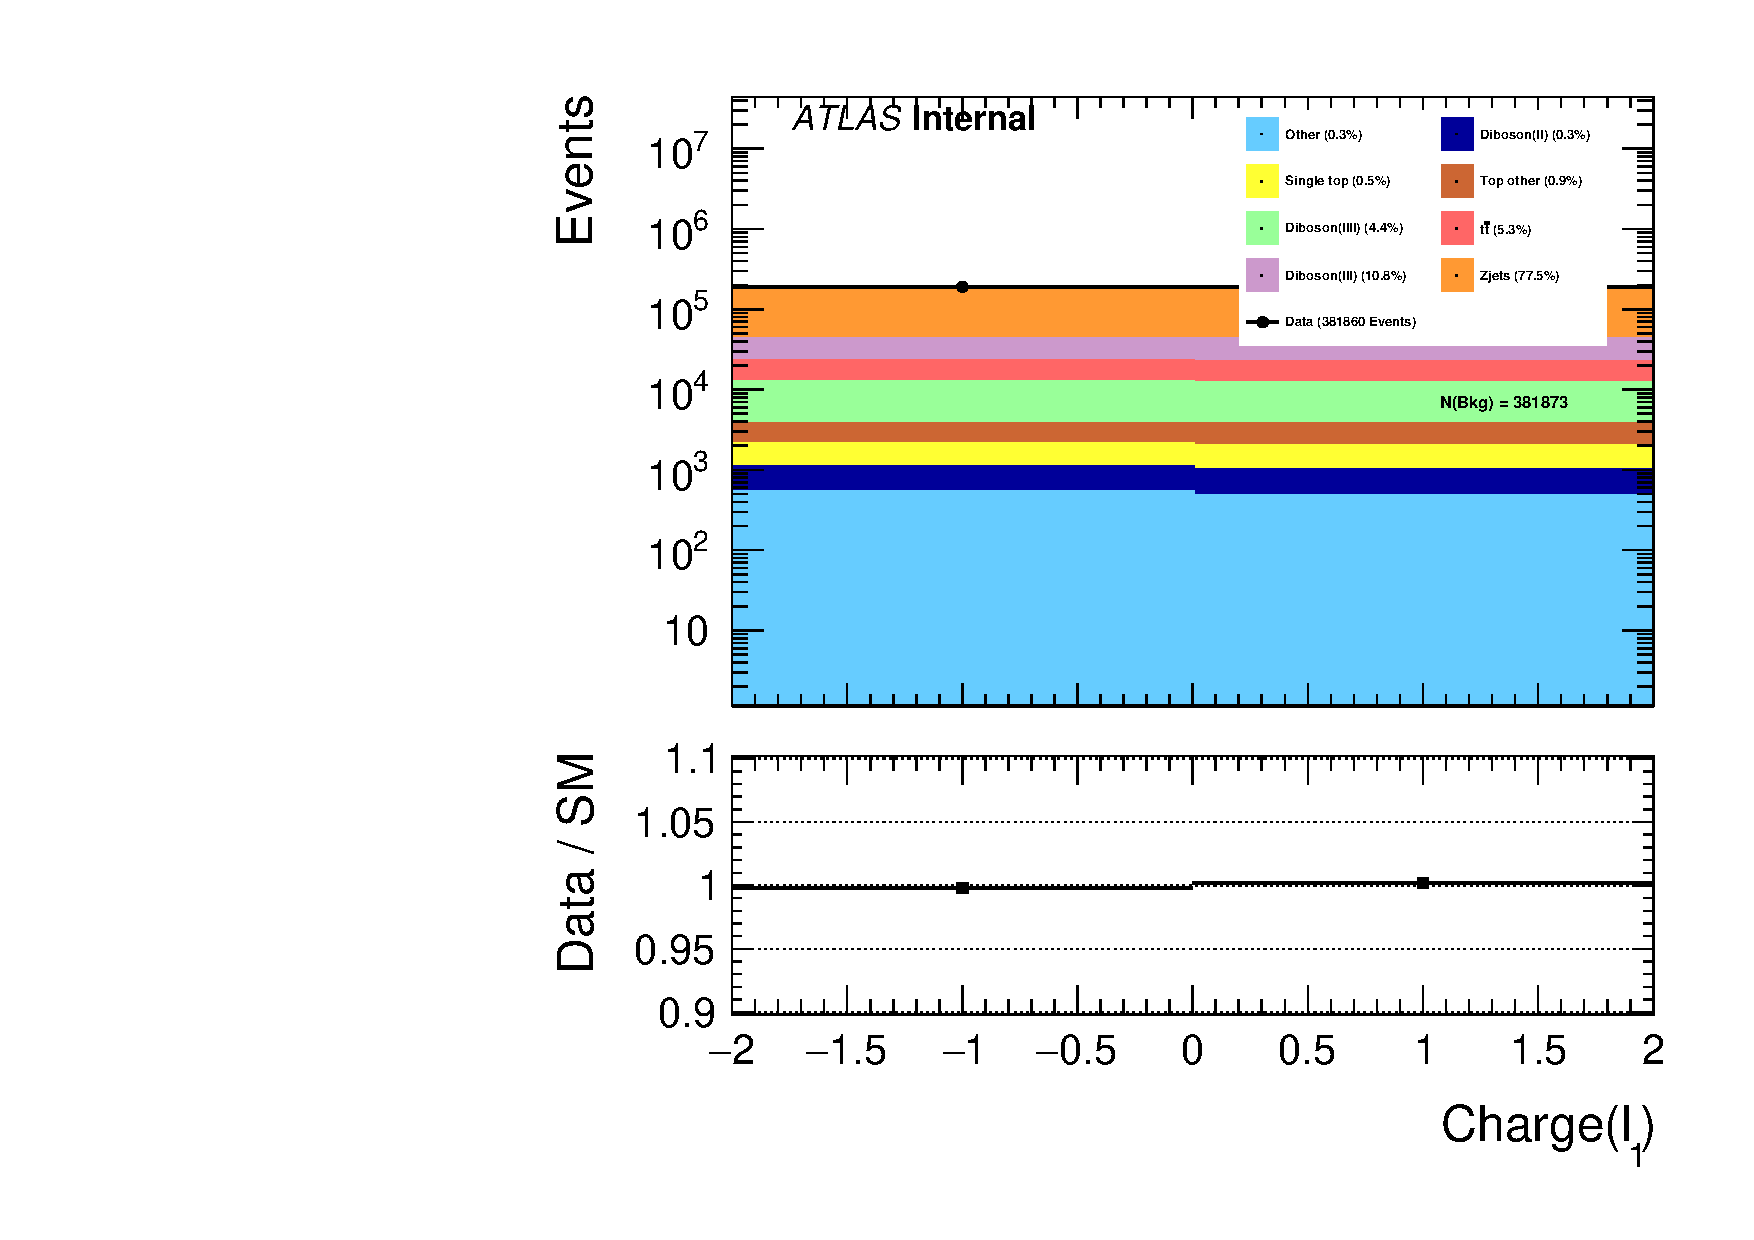
\includegraphics[width=\textwidth]{Figures/FeaturesHistograms/lep1_Charge.pdf}
        \caption{}
        \label{fig:lep1_Charge}
    \end{subfigure}
    \hfill
    \begin{subfigure}{.425\textwidth}
        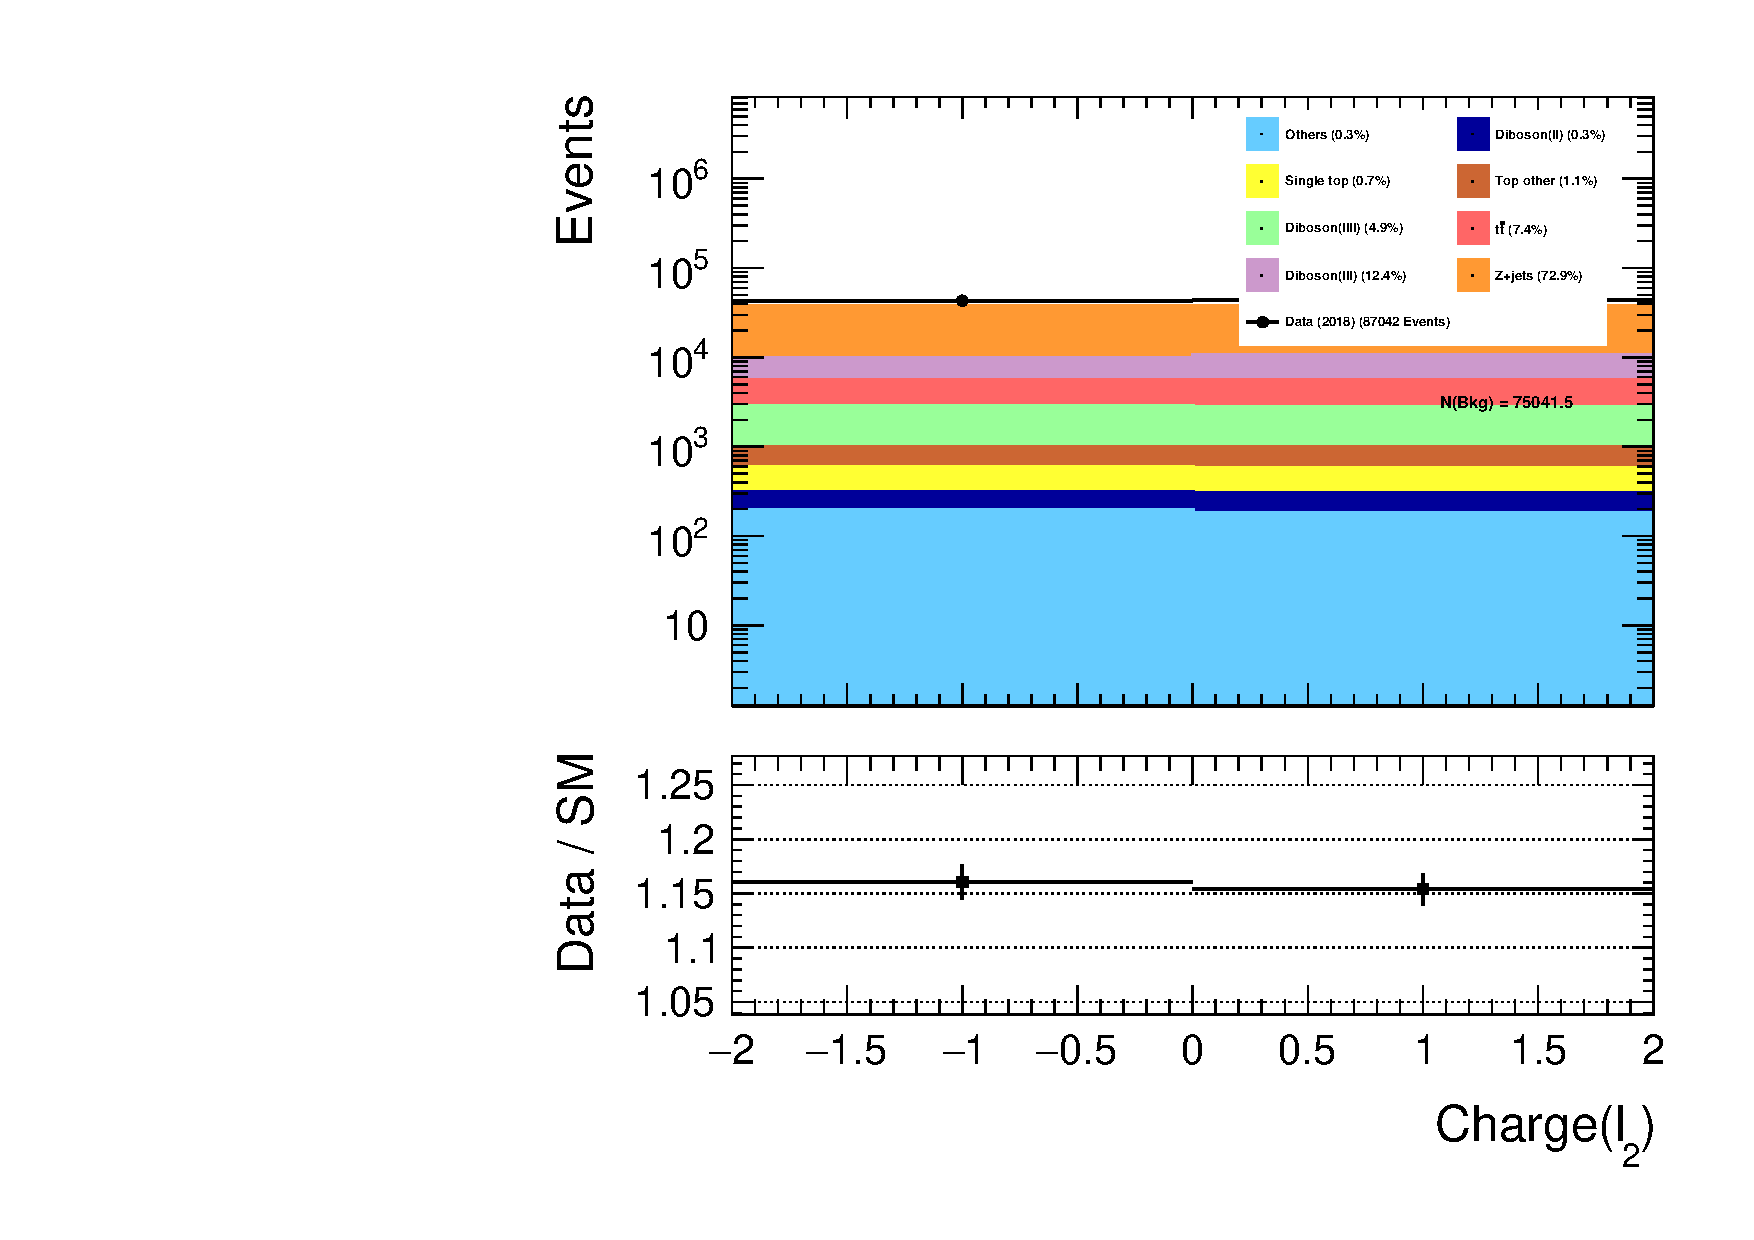
\includegraphics[width=\textwidth]{Figures/FeaturesHistograms/lep2_Charge.pdf}
        \caption{}
        \label{fig:lep2_Charge}
    \end{subfigure}
    }
    \makebox[0.9\linewidth][c]{%
    \begin{subfigure}{.425\textwidth}
        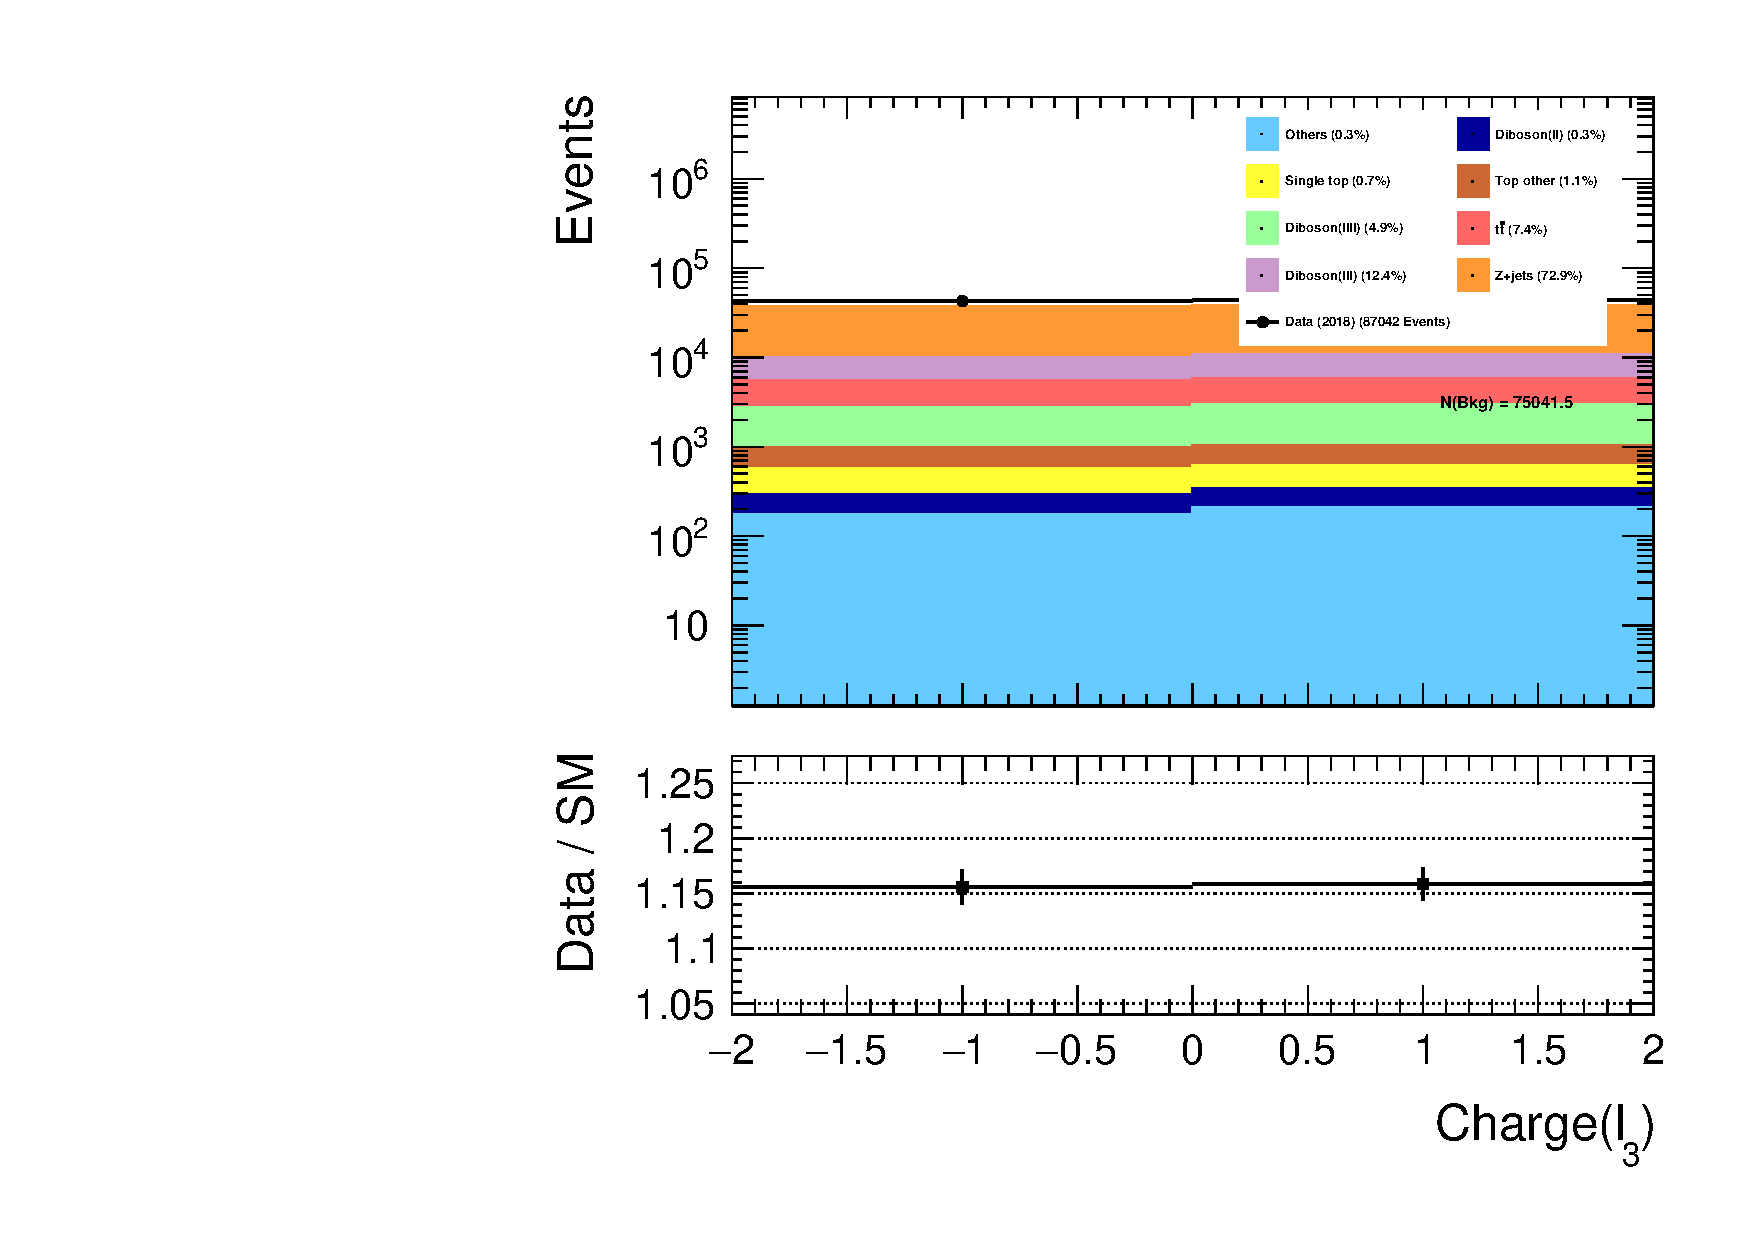
\includegraphics[width=\textwidth]{Figures/FeaturesHistograms/lep3_Charge.pdf}
        \caption{}
        \label{fig:lep3_Charge}
    \end{subfigure}
    \hfill
    \begin{subfigure}{.425\textwidth}
        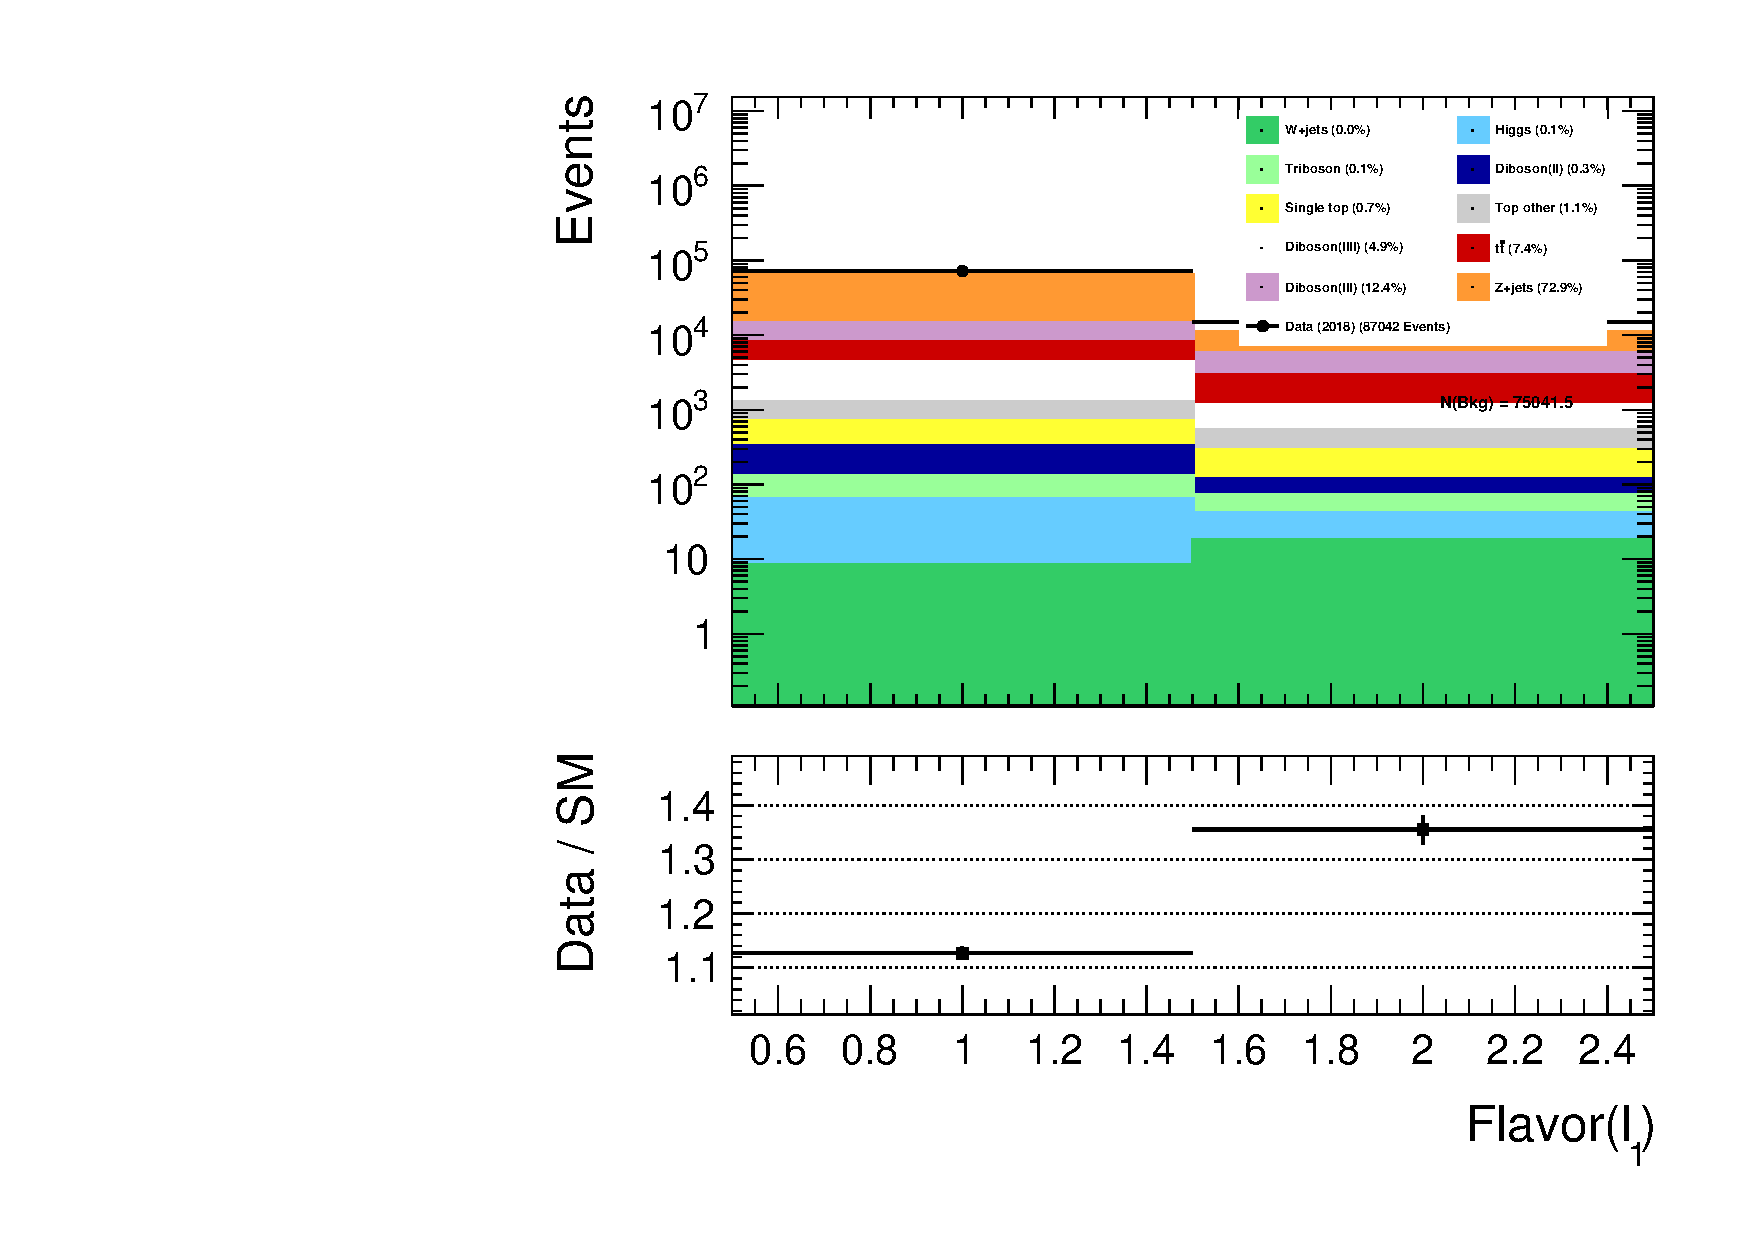
\includegraphics[width=\textwidth]{Figures/FeaturesHistograms/lep1_Flavor.pdf}
        \caption{}
        \label{fig:lep1_Flavor}
    \end{subfigure}
    }
    \makebox[0.9\linewidth][c]{%
    \begin{subfigure}{.425\textwidth}
        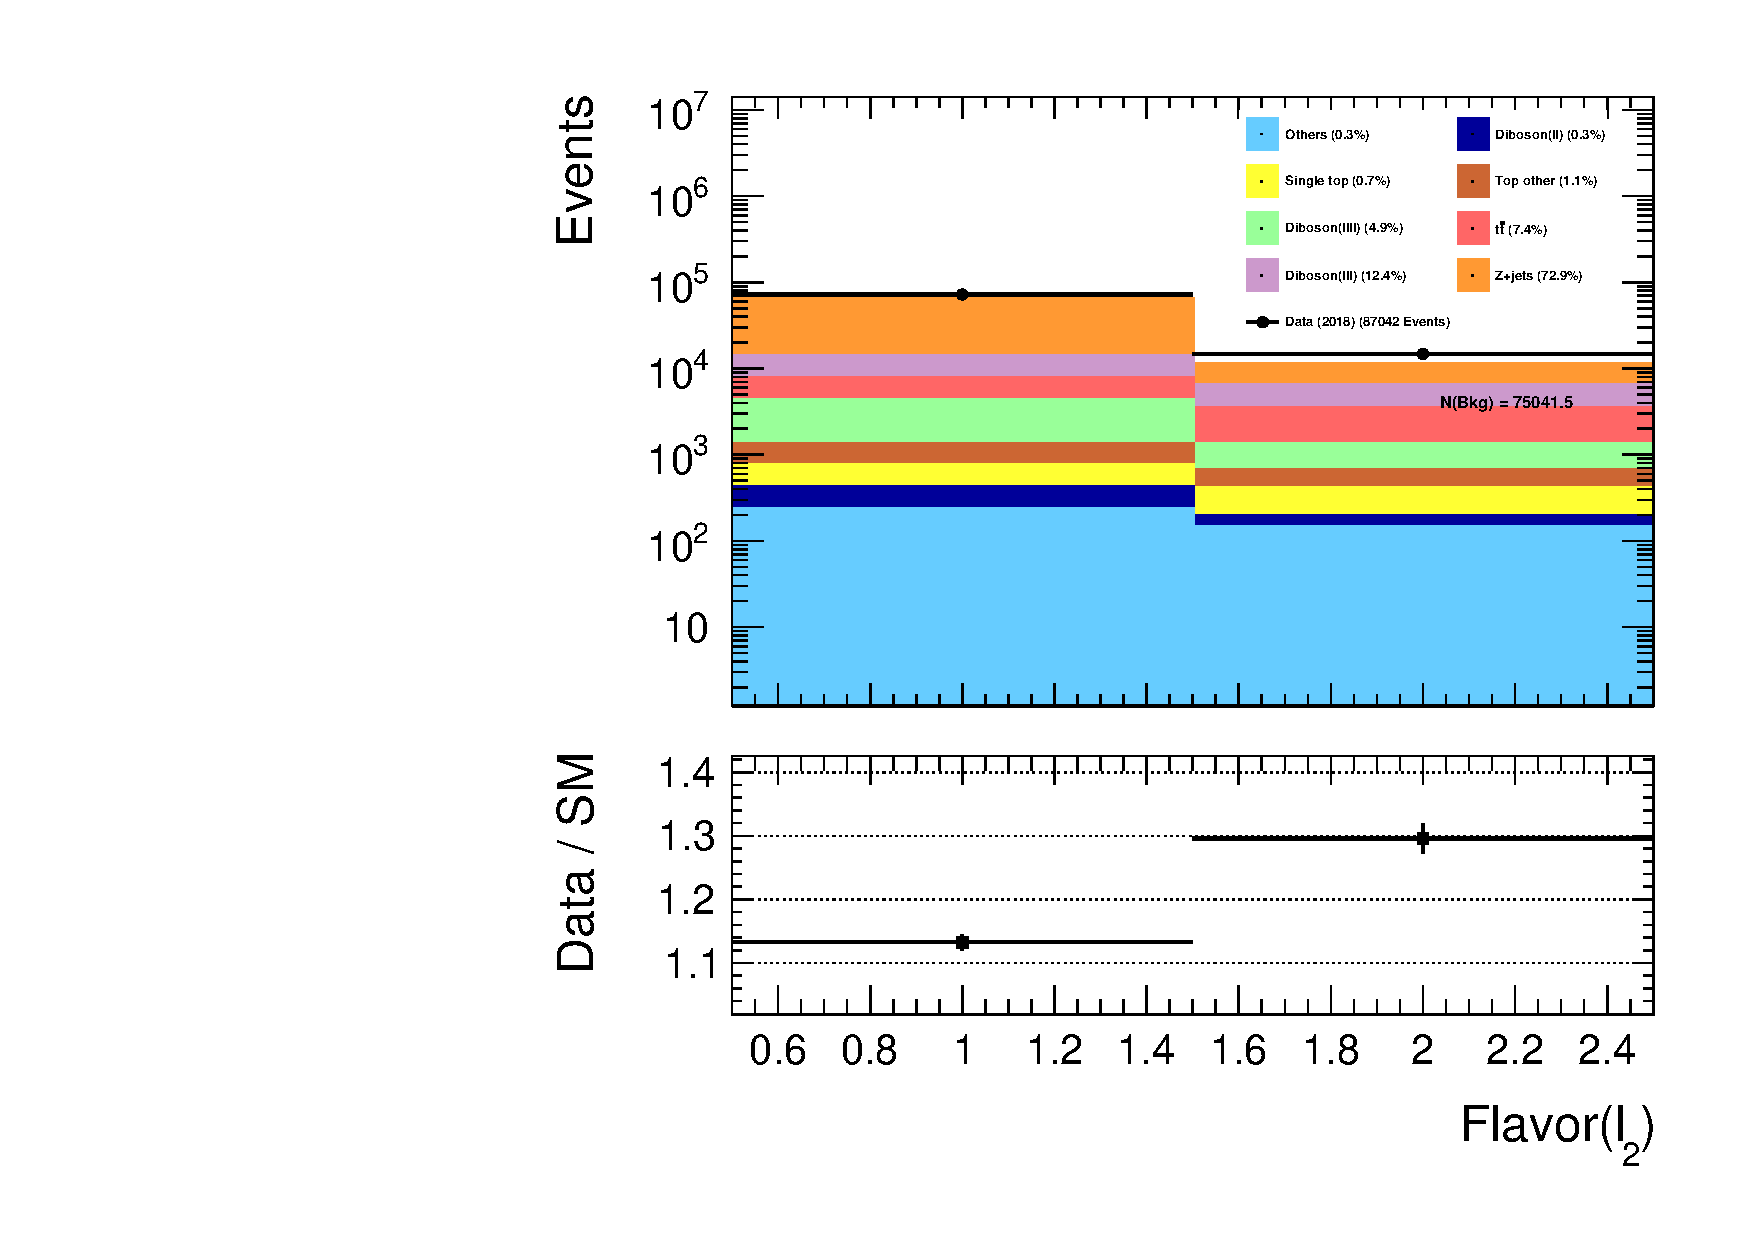
\includegraphics[width=\textwidth]{Figures/FeaturesHistograms/lep2_Flavor.pdf}
        \caption{}
        \label{fig:lep2_Flavor}
    \end{subfigure}
    \hfill
    \begin{subfigure}{.425\textwidth}
        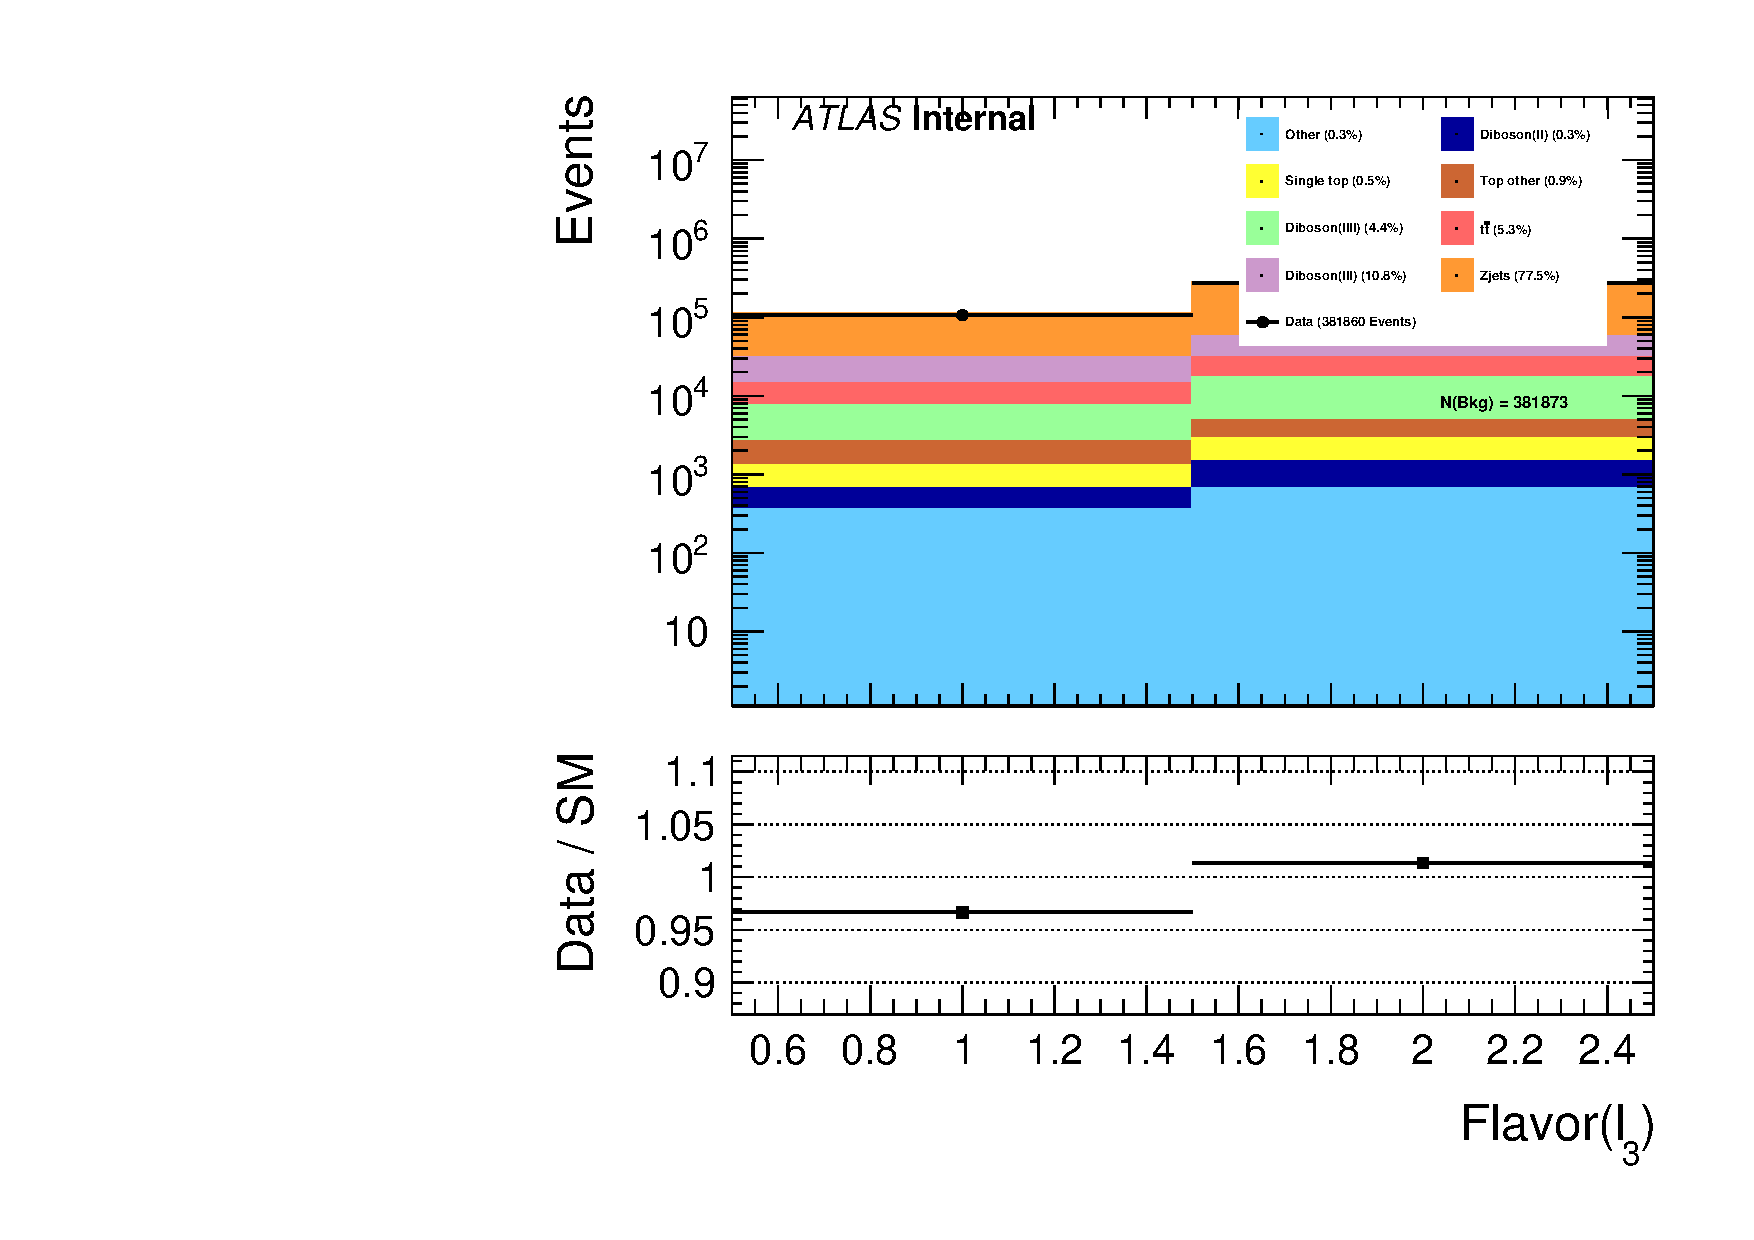
\includegraphics[width=\textwidth]{Figures/FeaturesHistograms/lep3_Flavor.pdf}
        \caption{}
        \label{fig:lep3_Flavor}
    \end{subfigure}
    }
    \caption{The event distribution for each channel over the charge for the first \ref{fig:lep1_Charge}
    , second \ref{fig:lep2_Charge} and third \ref{fig:lep3_Charge} lepton. Similarly, the distribution over the flavor
    for the first \ref{fig:lep1_Flavor}, second \ref{fig:lep2_Flavor} and third \ref{fig:lep3_Flavor} lepton}
\end{figure}
\newpage
\begin{figure}
    \makebox[0.9\linewidth][c]{%
    \centering
    \begin{subfigure}{.425\textwidth}
        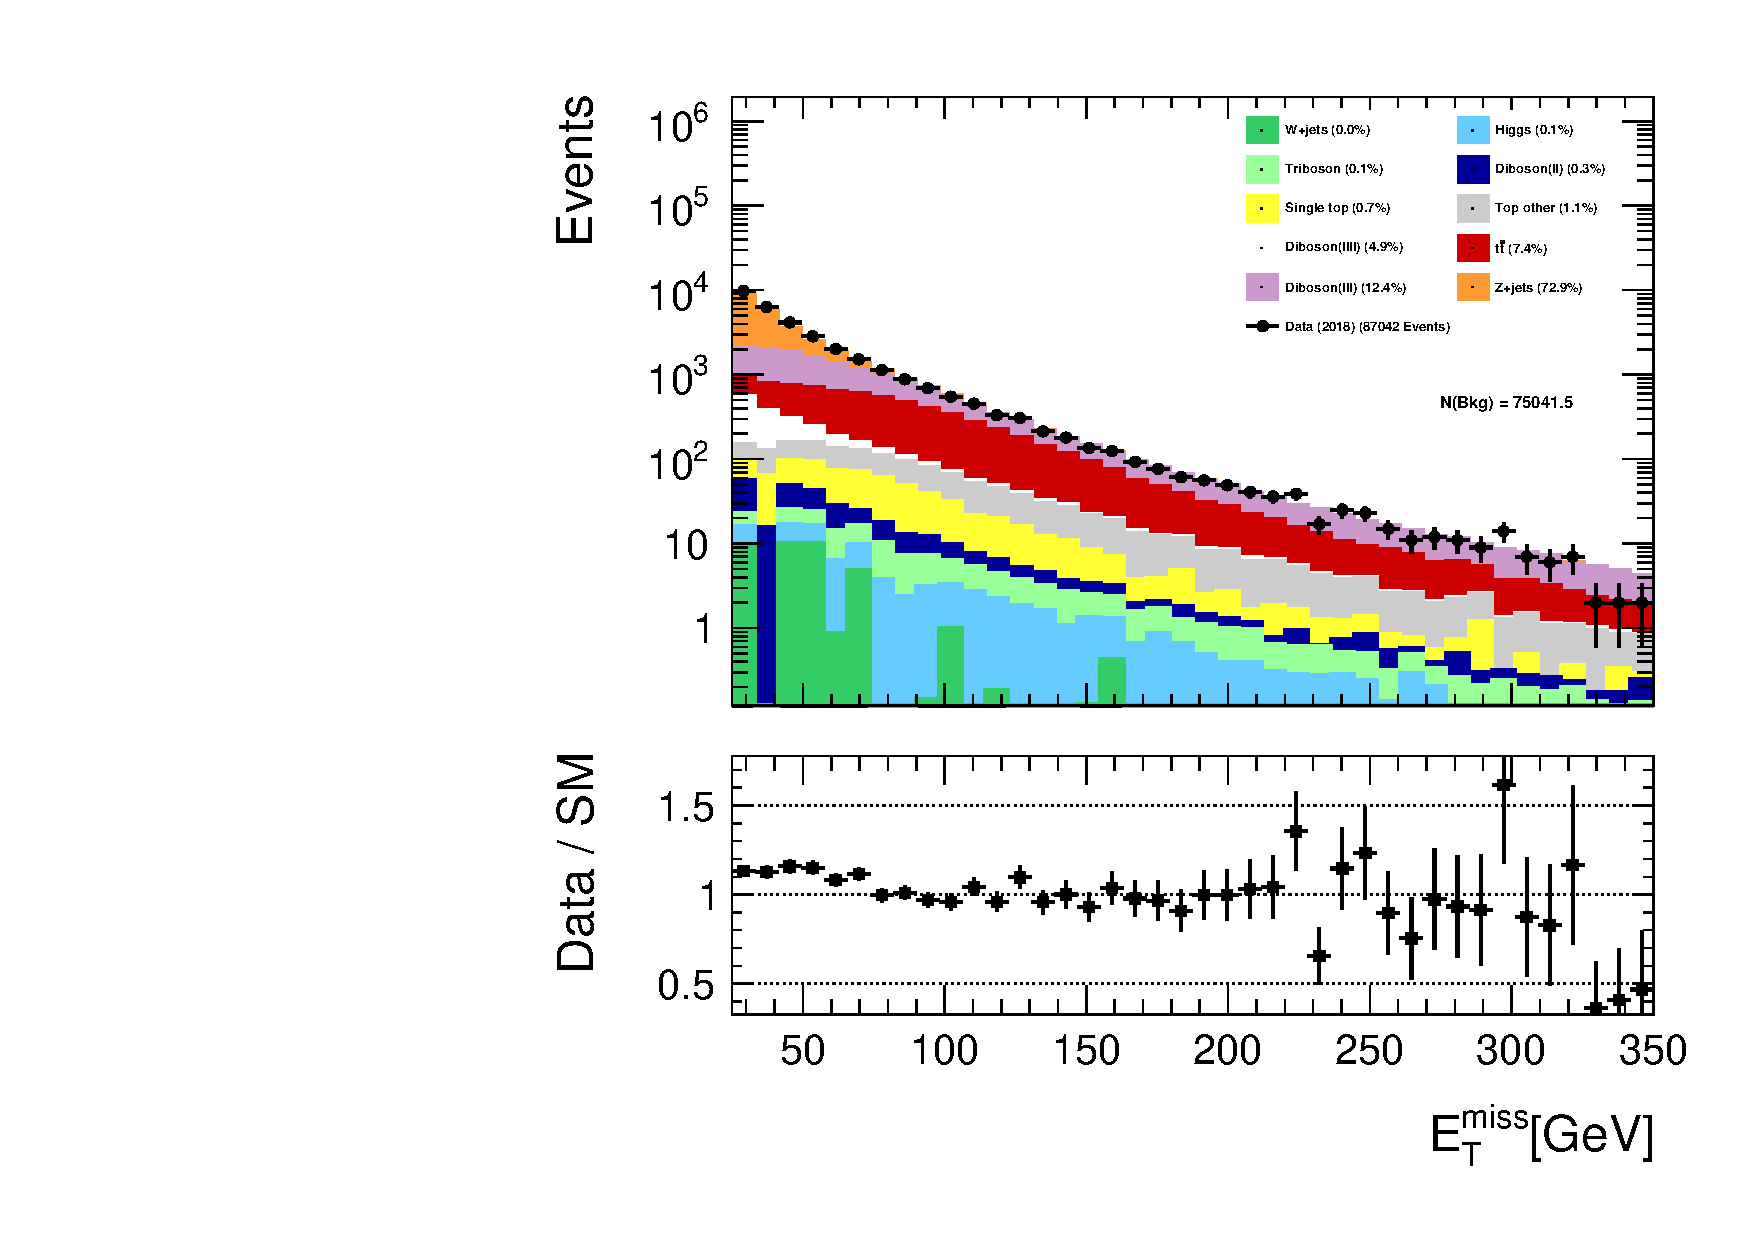
\includegraphics[width=\textwidth]{Figures/FeaturesHistograms/met_Et.pdf}
        \caption{}
        \label{fig:met_Et}
    \end{subfigure}
    \hfill
    \begin{subfigure}{.425\textwidth}
        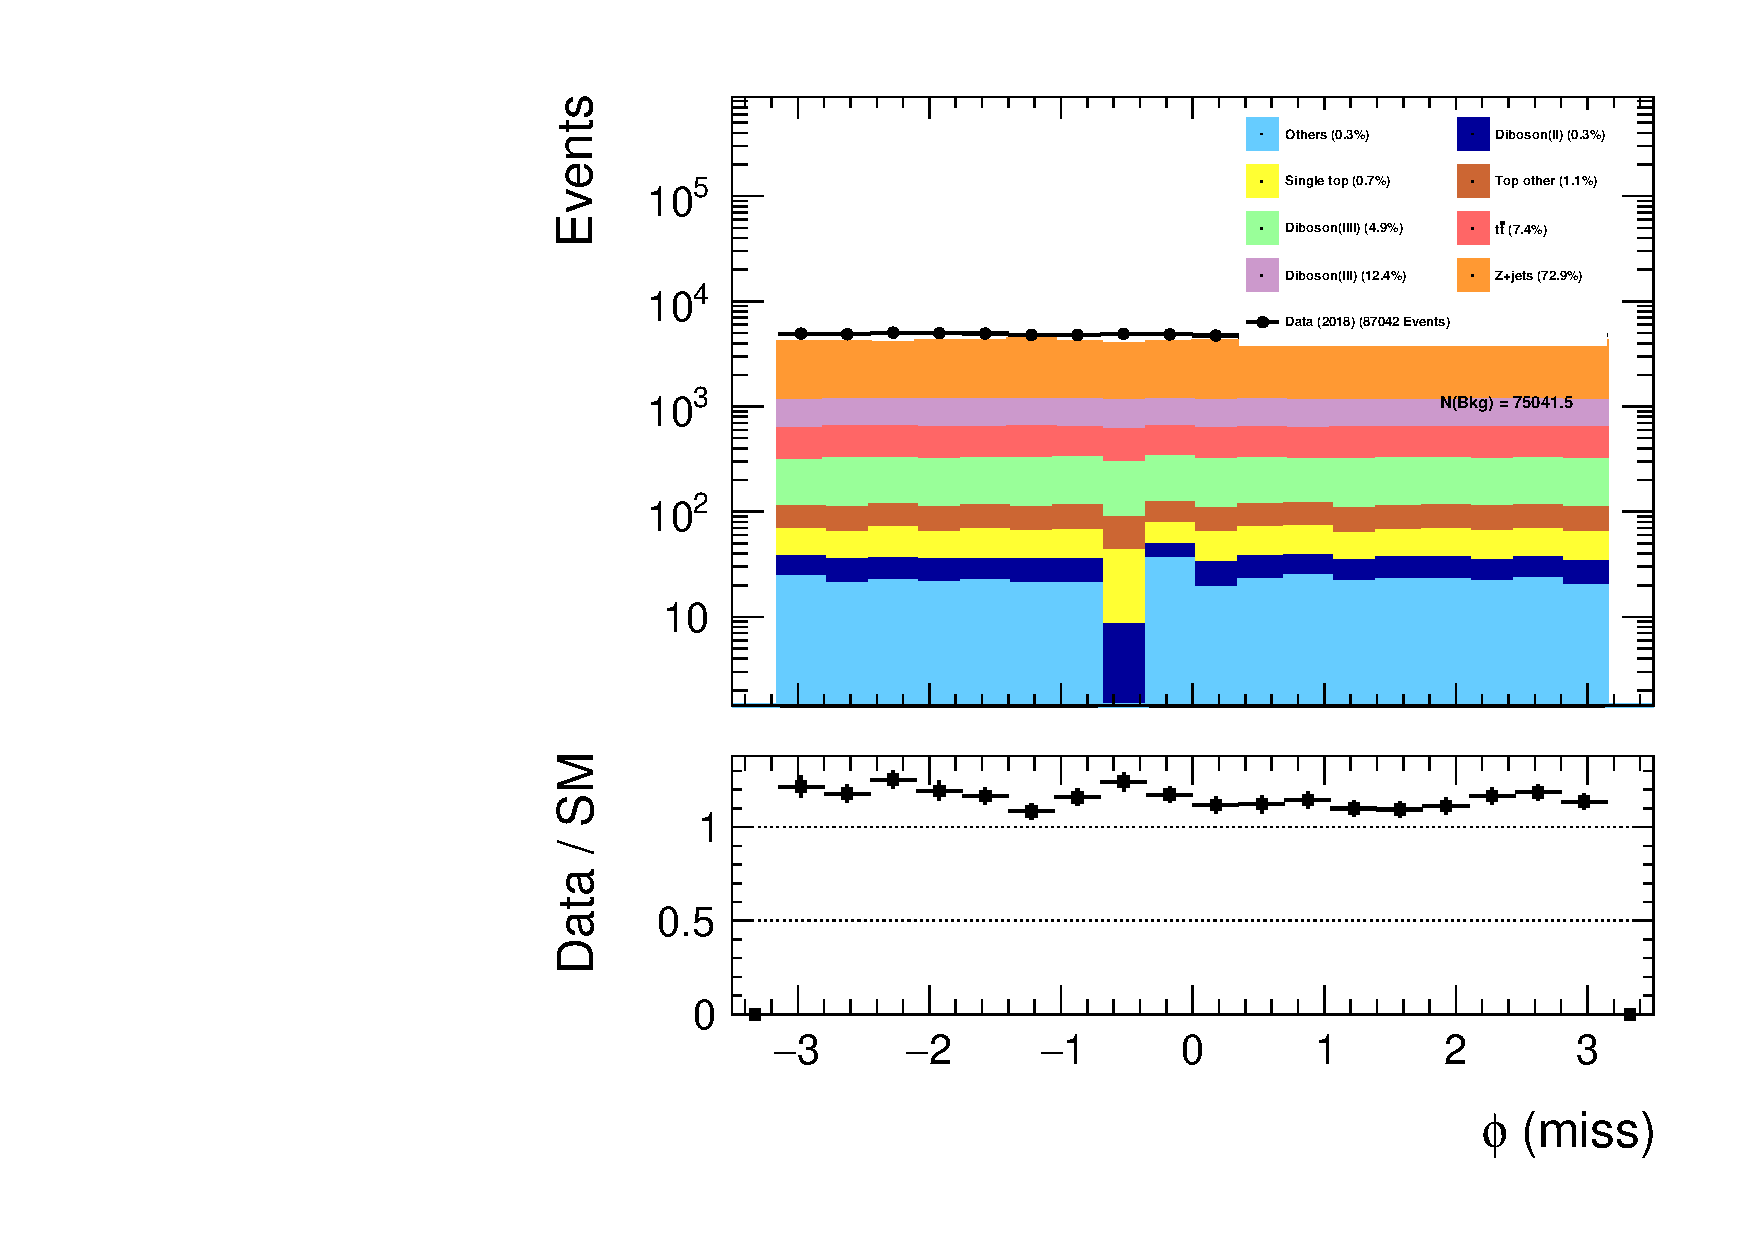
\includegraphics[width=\textwidth]{Figures/FeaturesHistograms/met_Phi.pdf}
        \caption{}
        \label{fig:met_Phi}
    \end{subfigure}
    }
    \makebox[0.9\linewidth][c]{%
    \begin{subfigure}{.425\textwidth}
        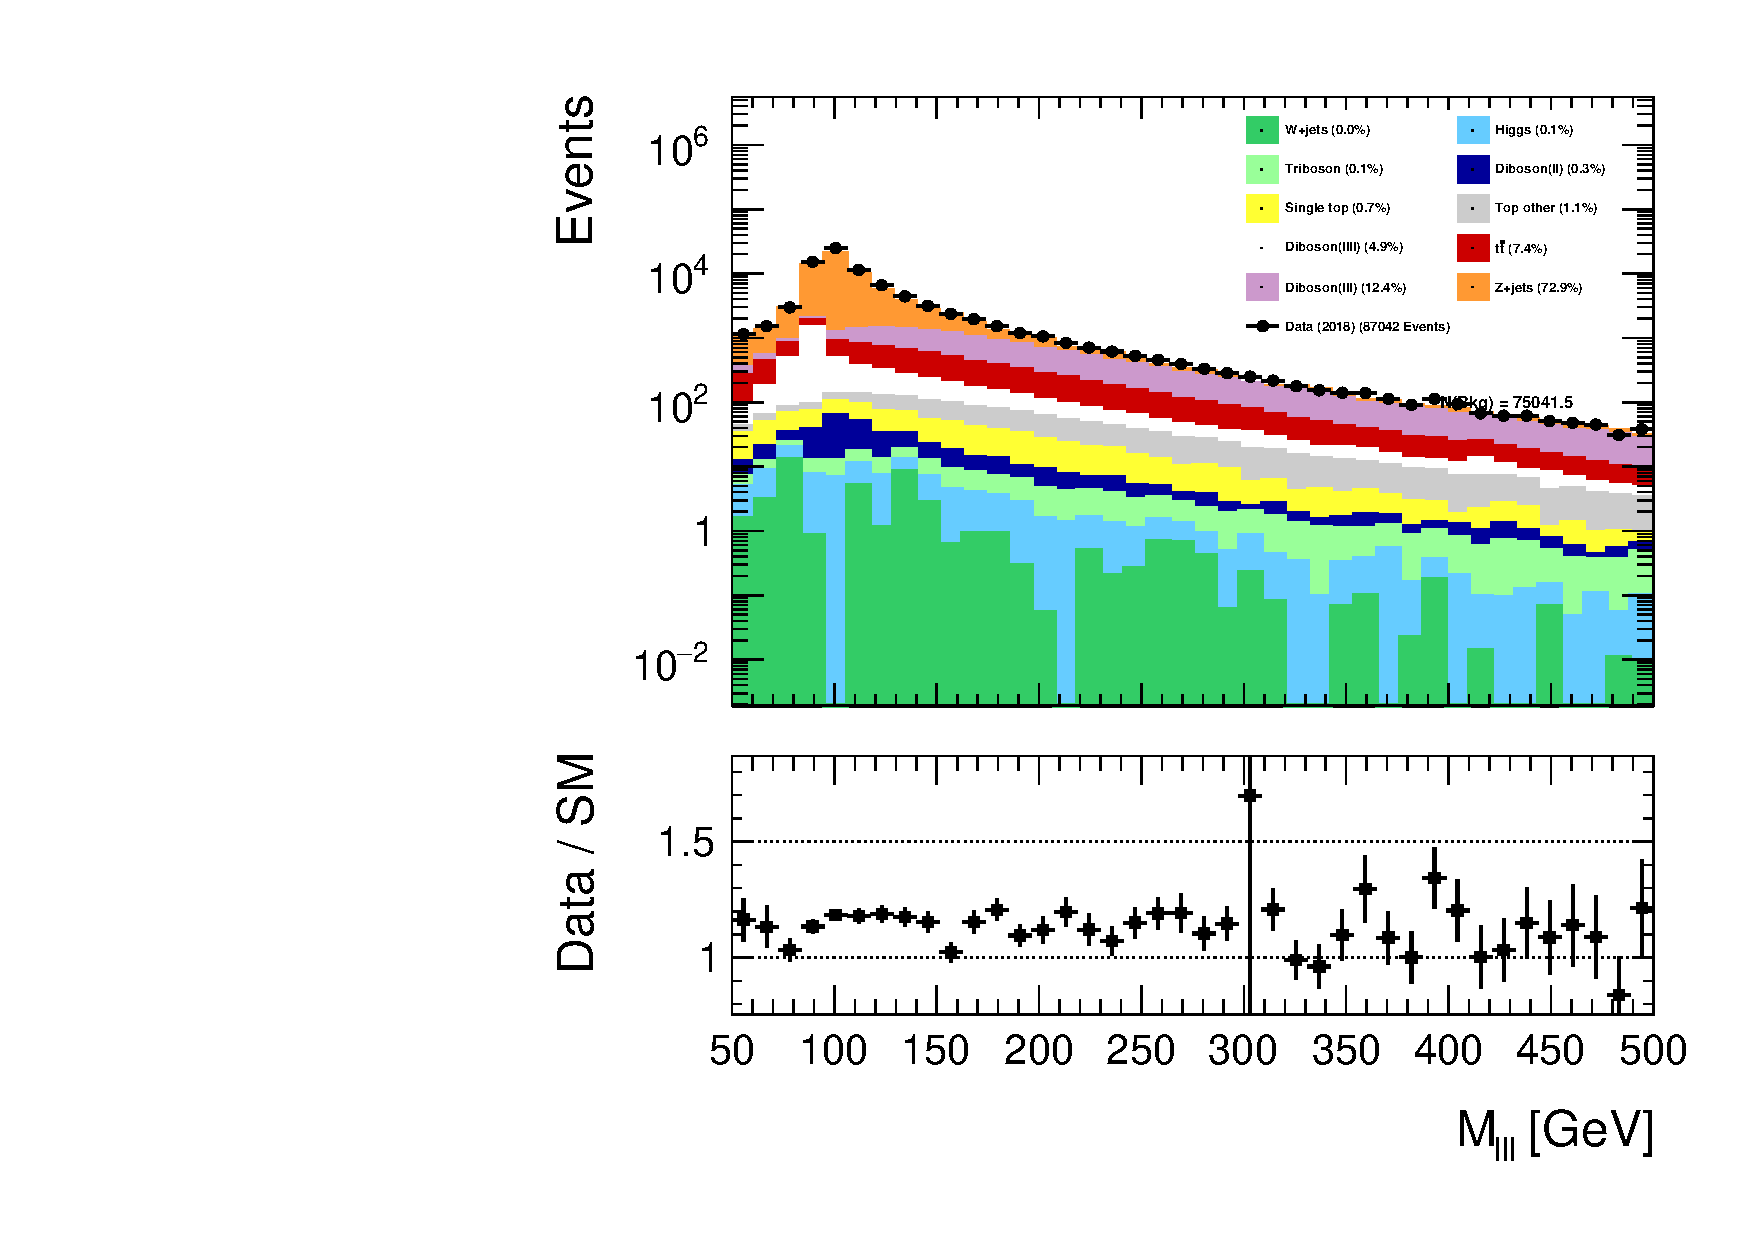
\includegraphics[width=\textwidth]{Figures/FeaturesHistograms/mlll.pdf}
        \caption{}
        \label{fig:mlll}
    \end{subfigure}
    \hfill
    \begin{subfigure}{.425\textwidth}
        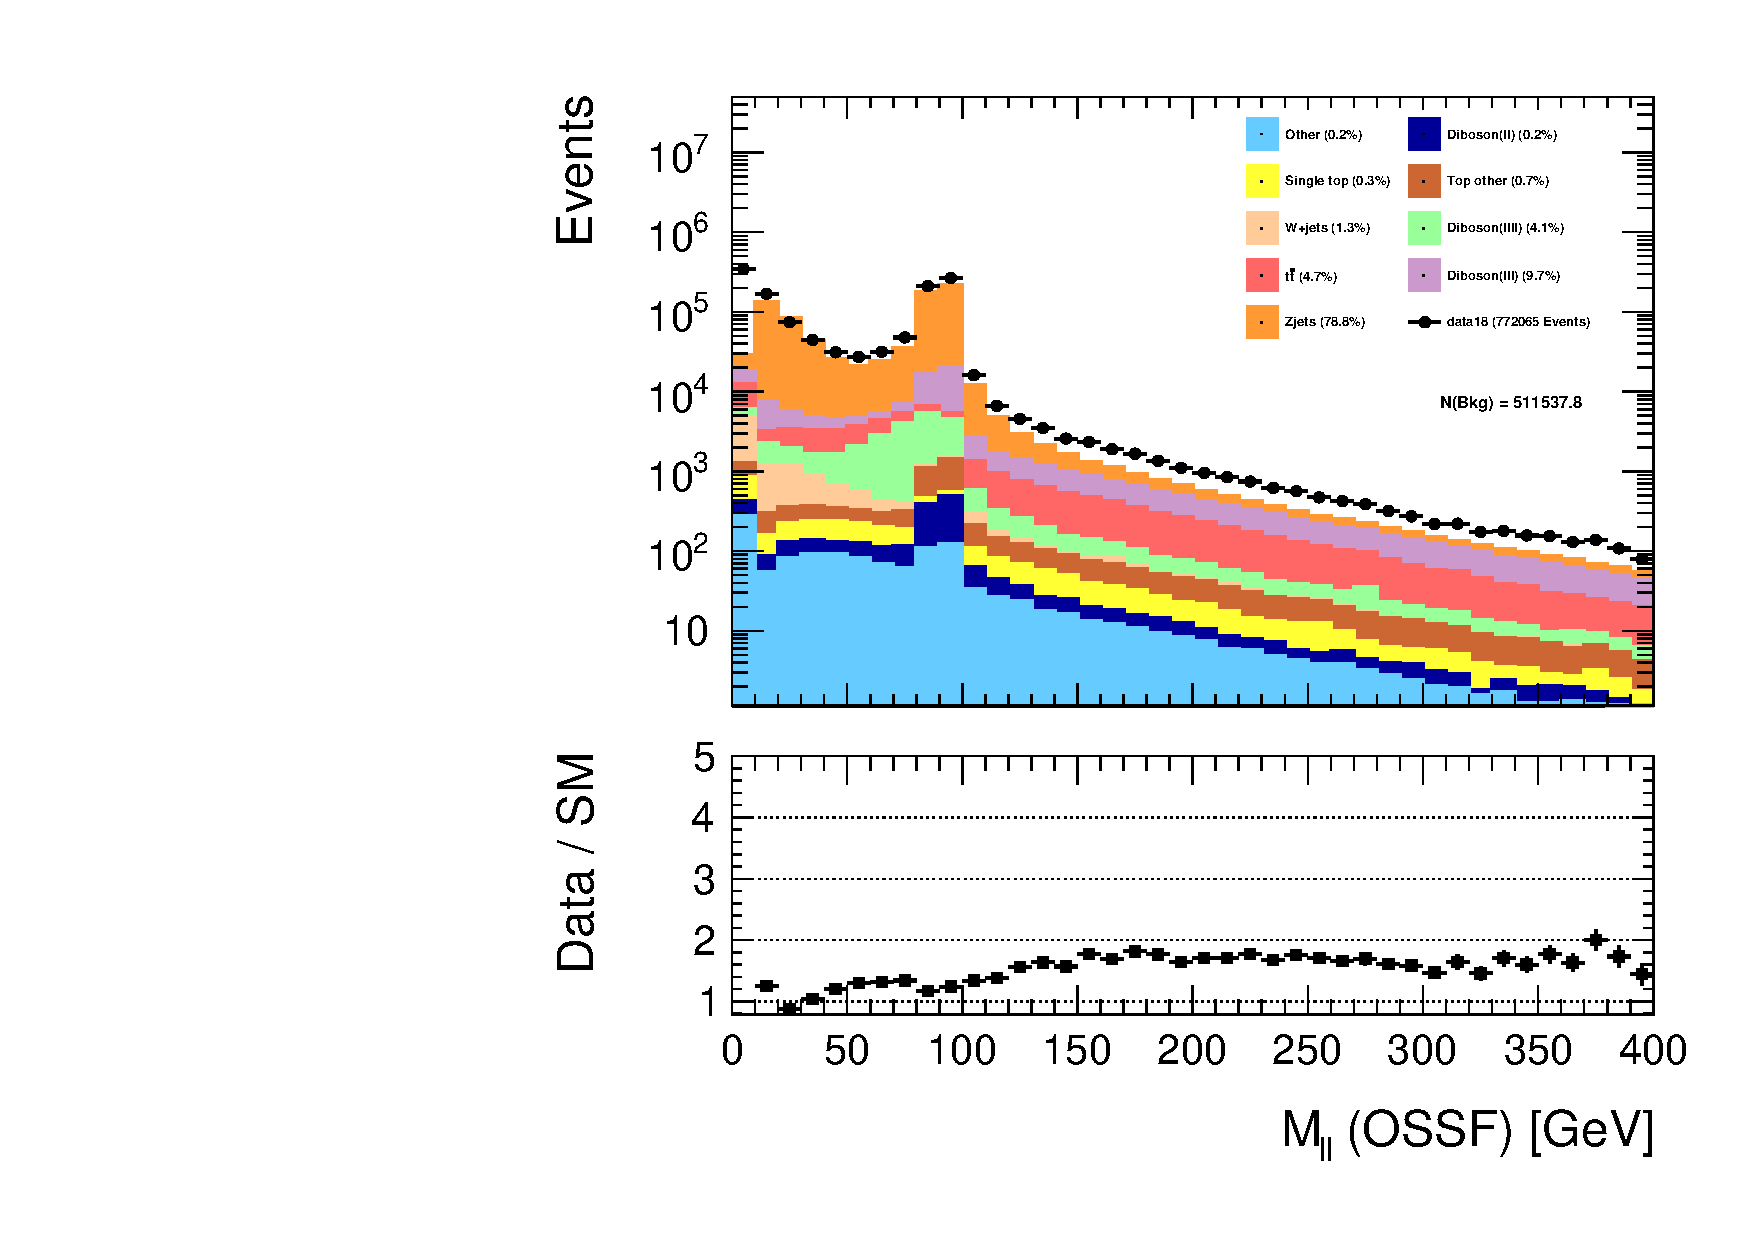
\includegraphics[width=\textwidth]{Figures/FeaturesHistograms/mll_OSSF.pdf}
        \caption{}
        \label{fig:mll_OSSF}
    \end{subfigure}
    }
    \makebox[0.9\linewidth][c]{%
    \begin{subfigure}{.425\textwidth}
        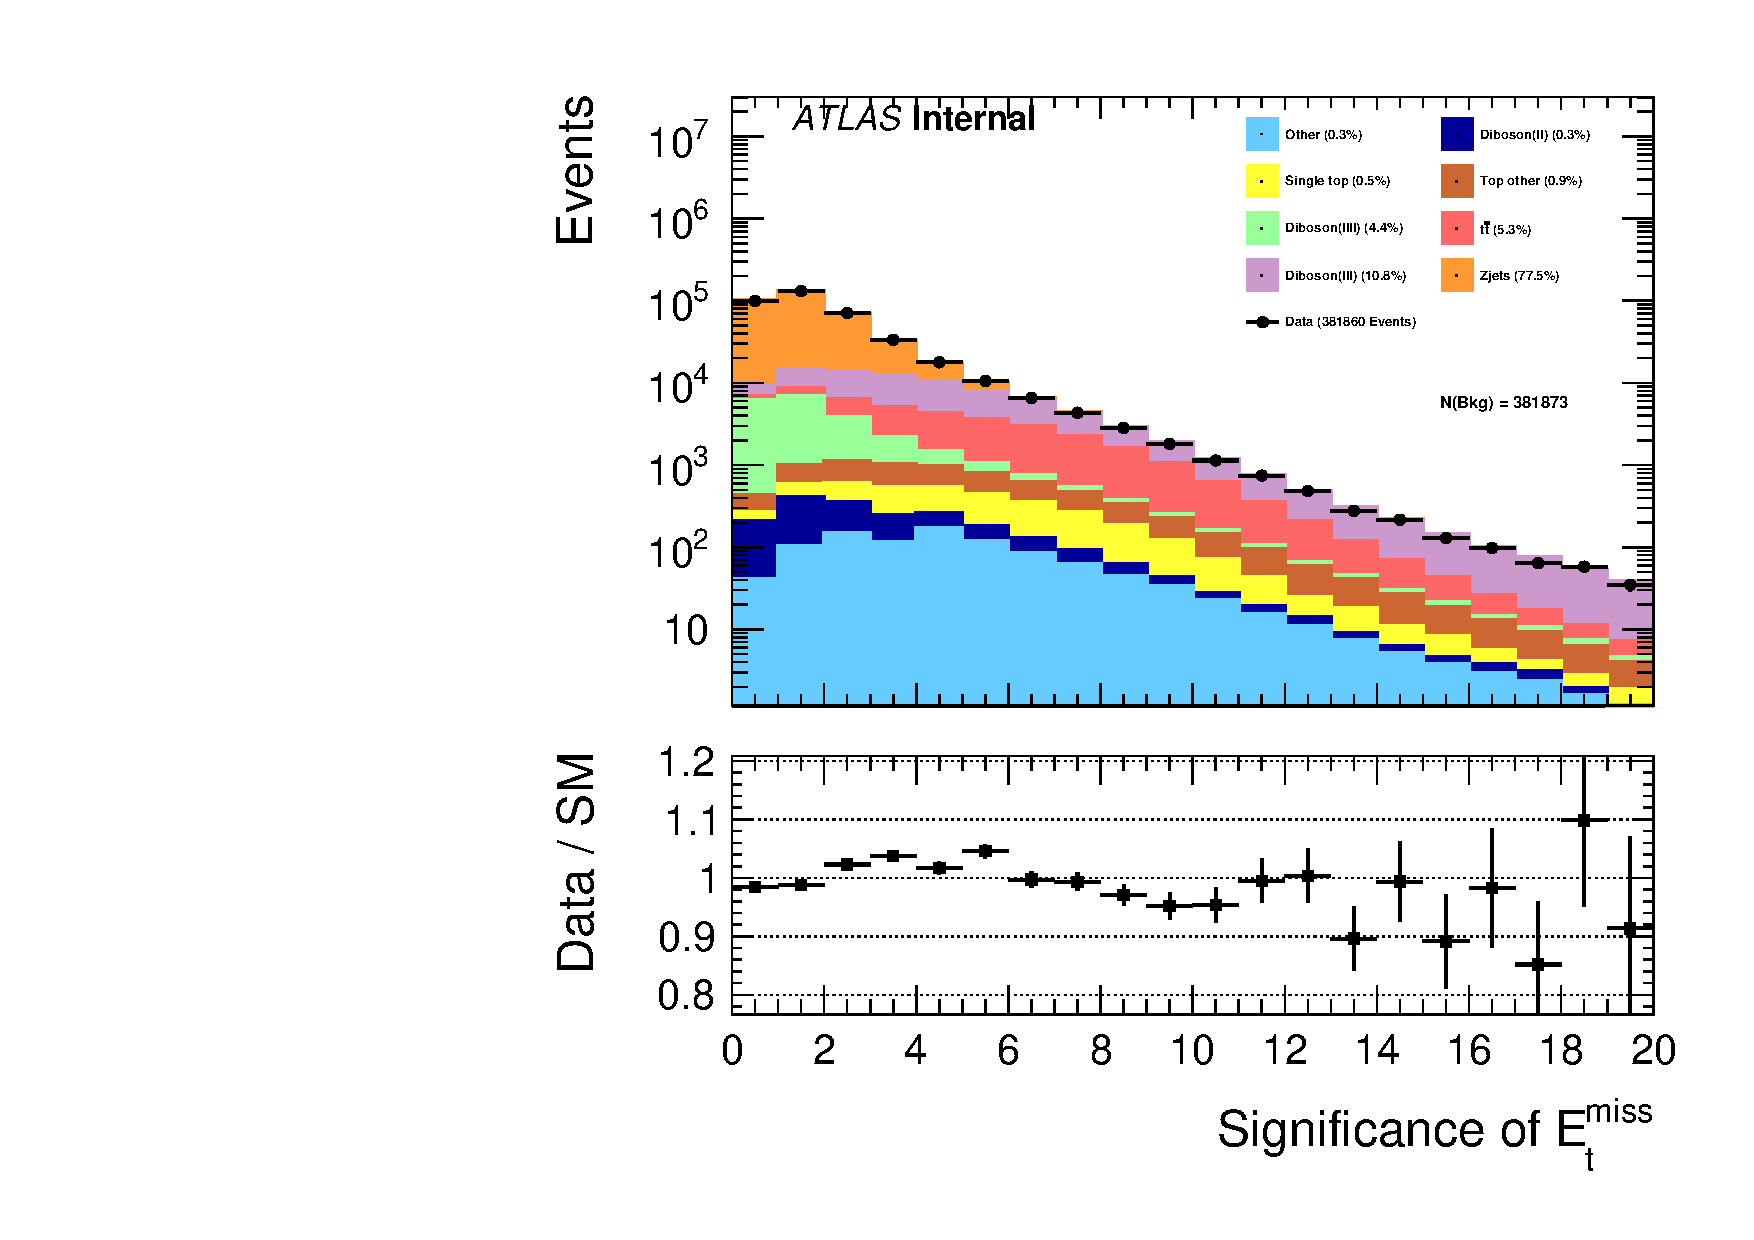
\includegraphics[width=\textwidth]{Figures/FeaturesHistograms/met_Sign.pdf}
        \caption{}
        \label{fig:met_Sign}
    \end{subfigure}
    \hfill
    \begin{subfigure}{.425\textwidth}
        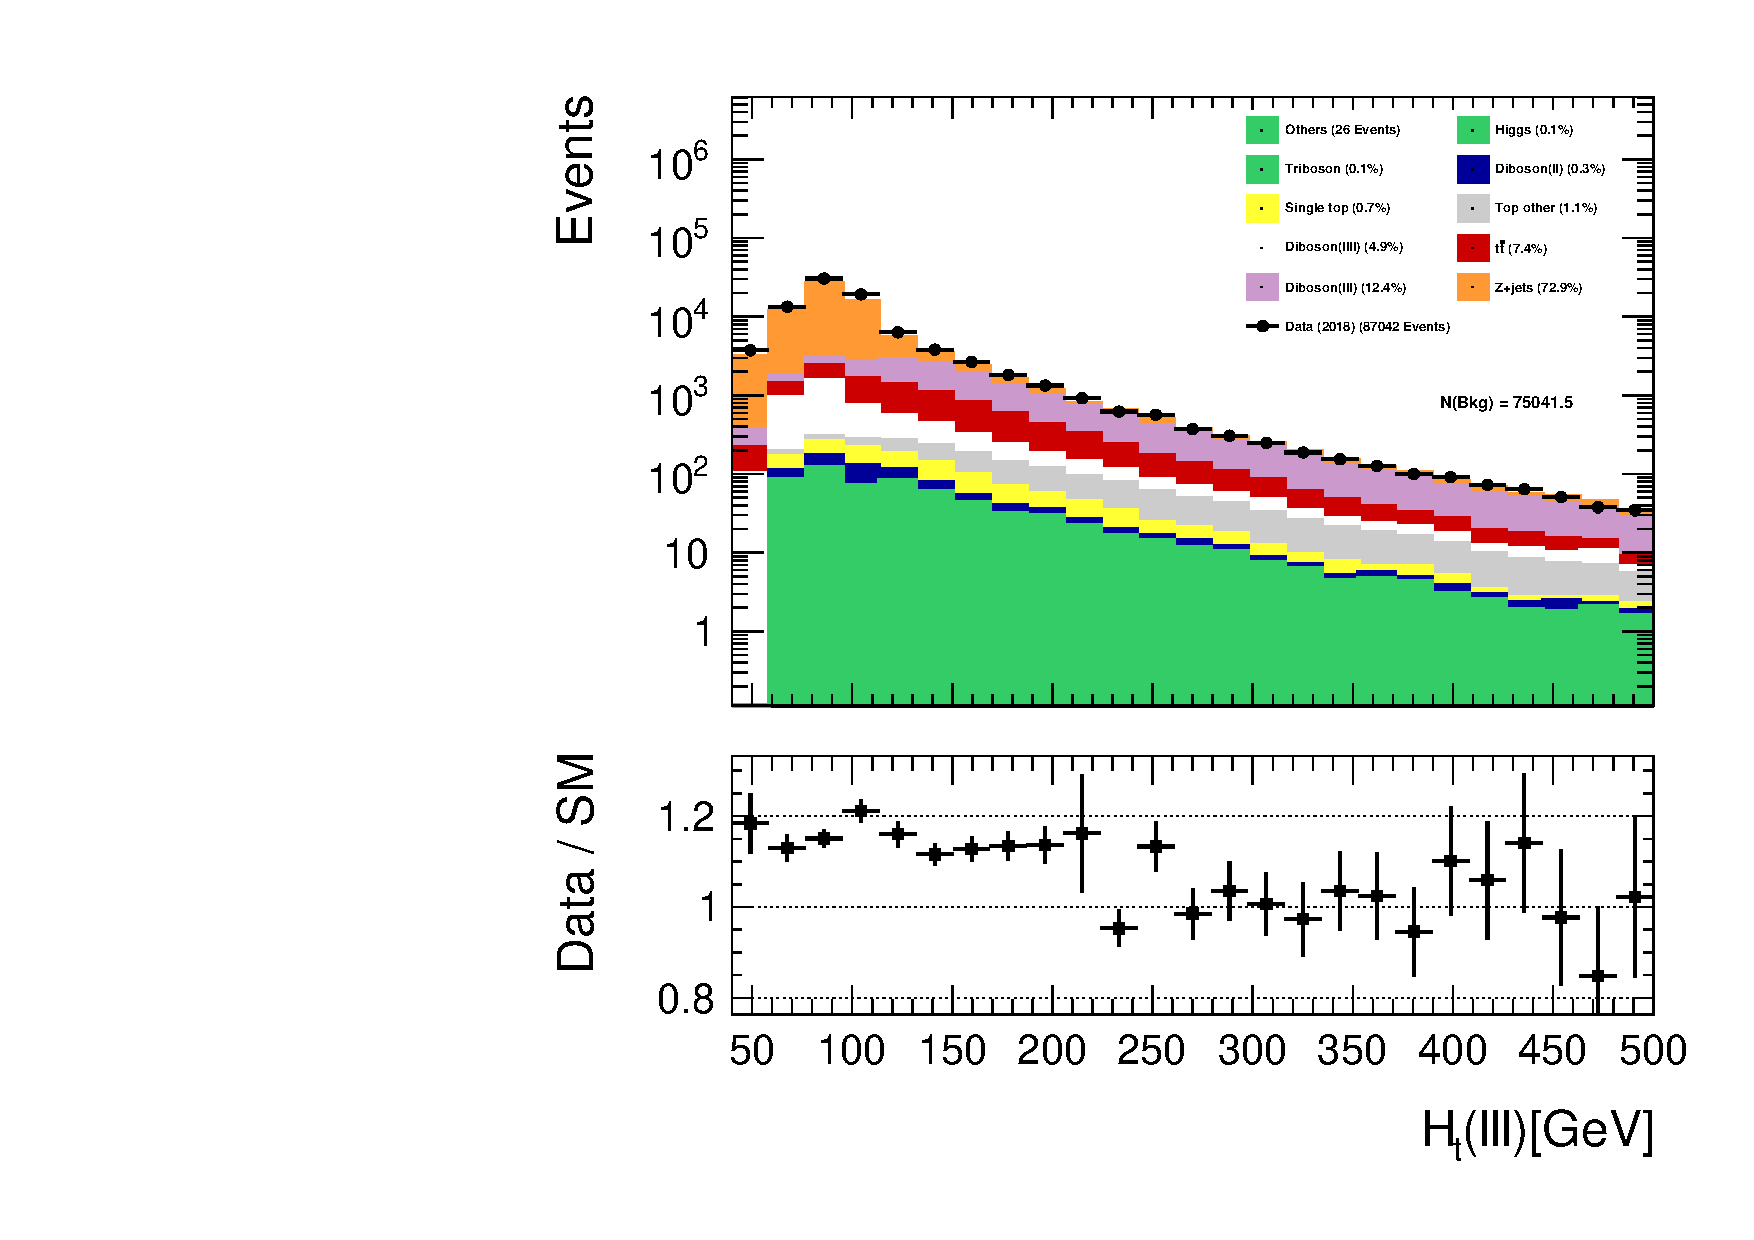
\includegraphics[width=\textwidth]{Figures/FeaturesHistograms/Ht_lll.pdf}
        \caption{}
        \label{fig:Ht_lll}
    \end{subfigure}
    }
    \caption{The event distribution for for each channel over the energy \ref{fig:met_Et} and azimuthal
    angel \ref{fig:met_Phi} for the transverse momentum. The distribution of the invariant mass of the
    three leptons \ref{fig:mlll} and the OSSF pair \ref{fig:mll_OSSF}. The distribution over the significance
    of the missing transverse enegy \ref{fig:met_Sign} and the sum of $P_t$ \ref{fig:Ht_lll}.}
\end{figure}
\newpage
\begin{figure}
    \makebox[0.9\linewidth][c]{%
    \centering
    \begin{subfigure}{.425\textwidth}
        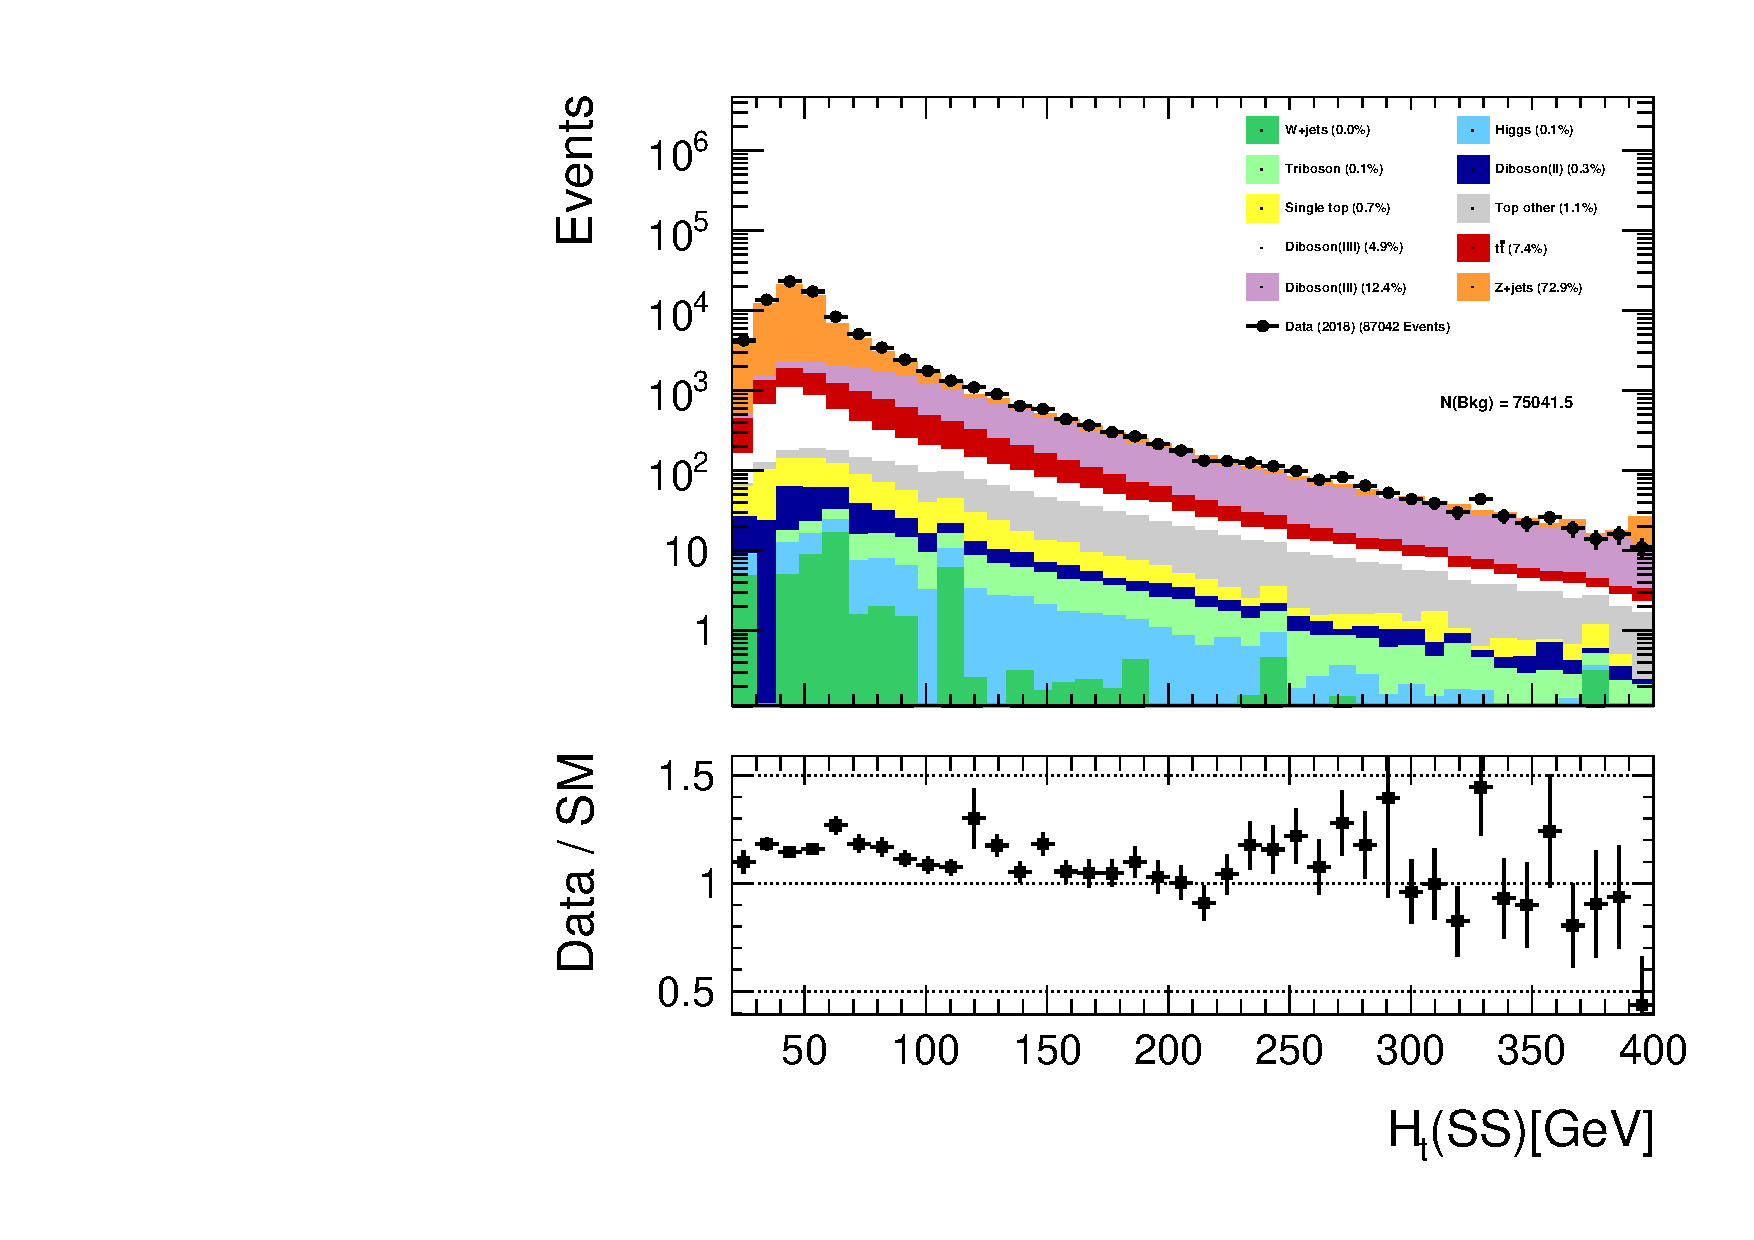
\includegraphics[width=\textwidth]{Figures/FeaturesHistograms/Ht_SS.pdf}
        \caption{}
        \label{fig:Ht_SS}
    \end{subfigure}
    \hfill
    \begin{subfigure}{.425\textwidth}
        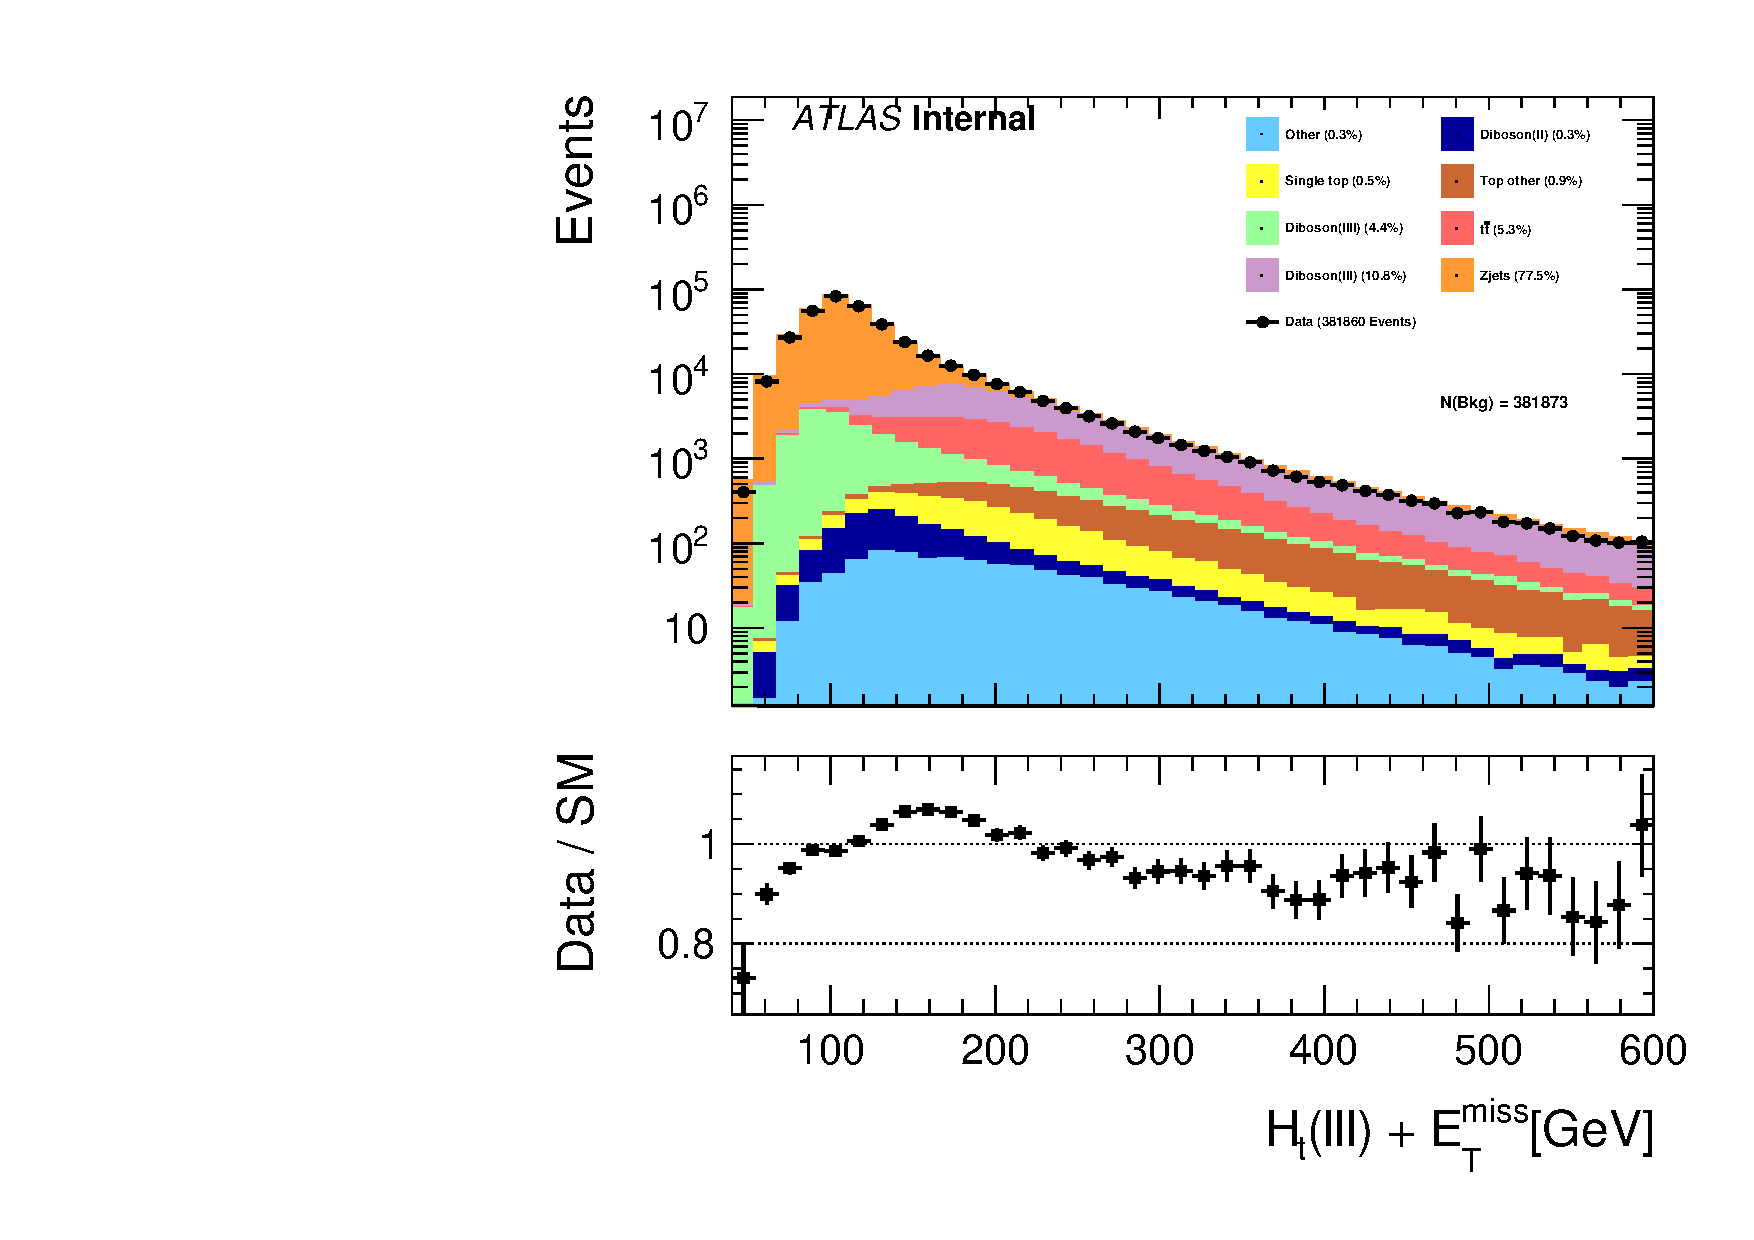
\includegraphics[width=\textwidth]{Figures/FeaturesHistograms/Ht_met_Et.pdf}
        \caption{}
        \label{fig:Ht_met_Et}
    \end{subfigure}
    }
    \makebox[0.9\linewidth][c]{%
    \begin{subfigure}{.425\textwidth}
        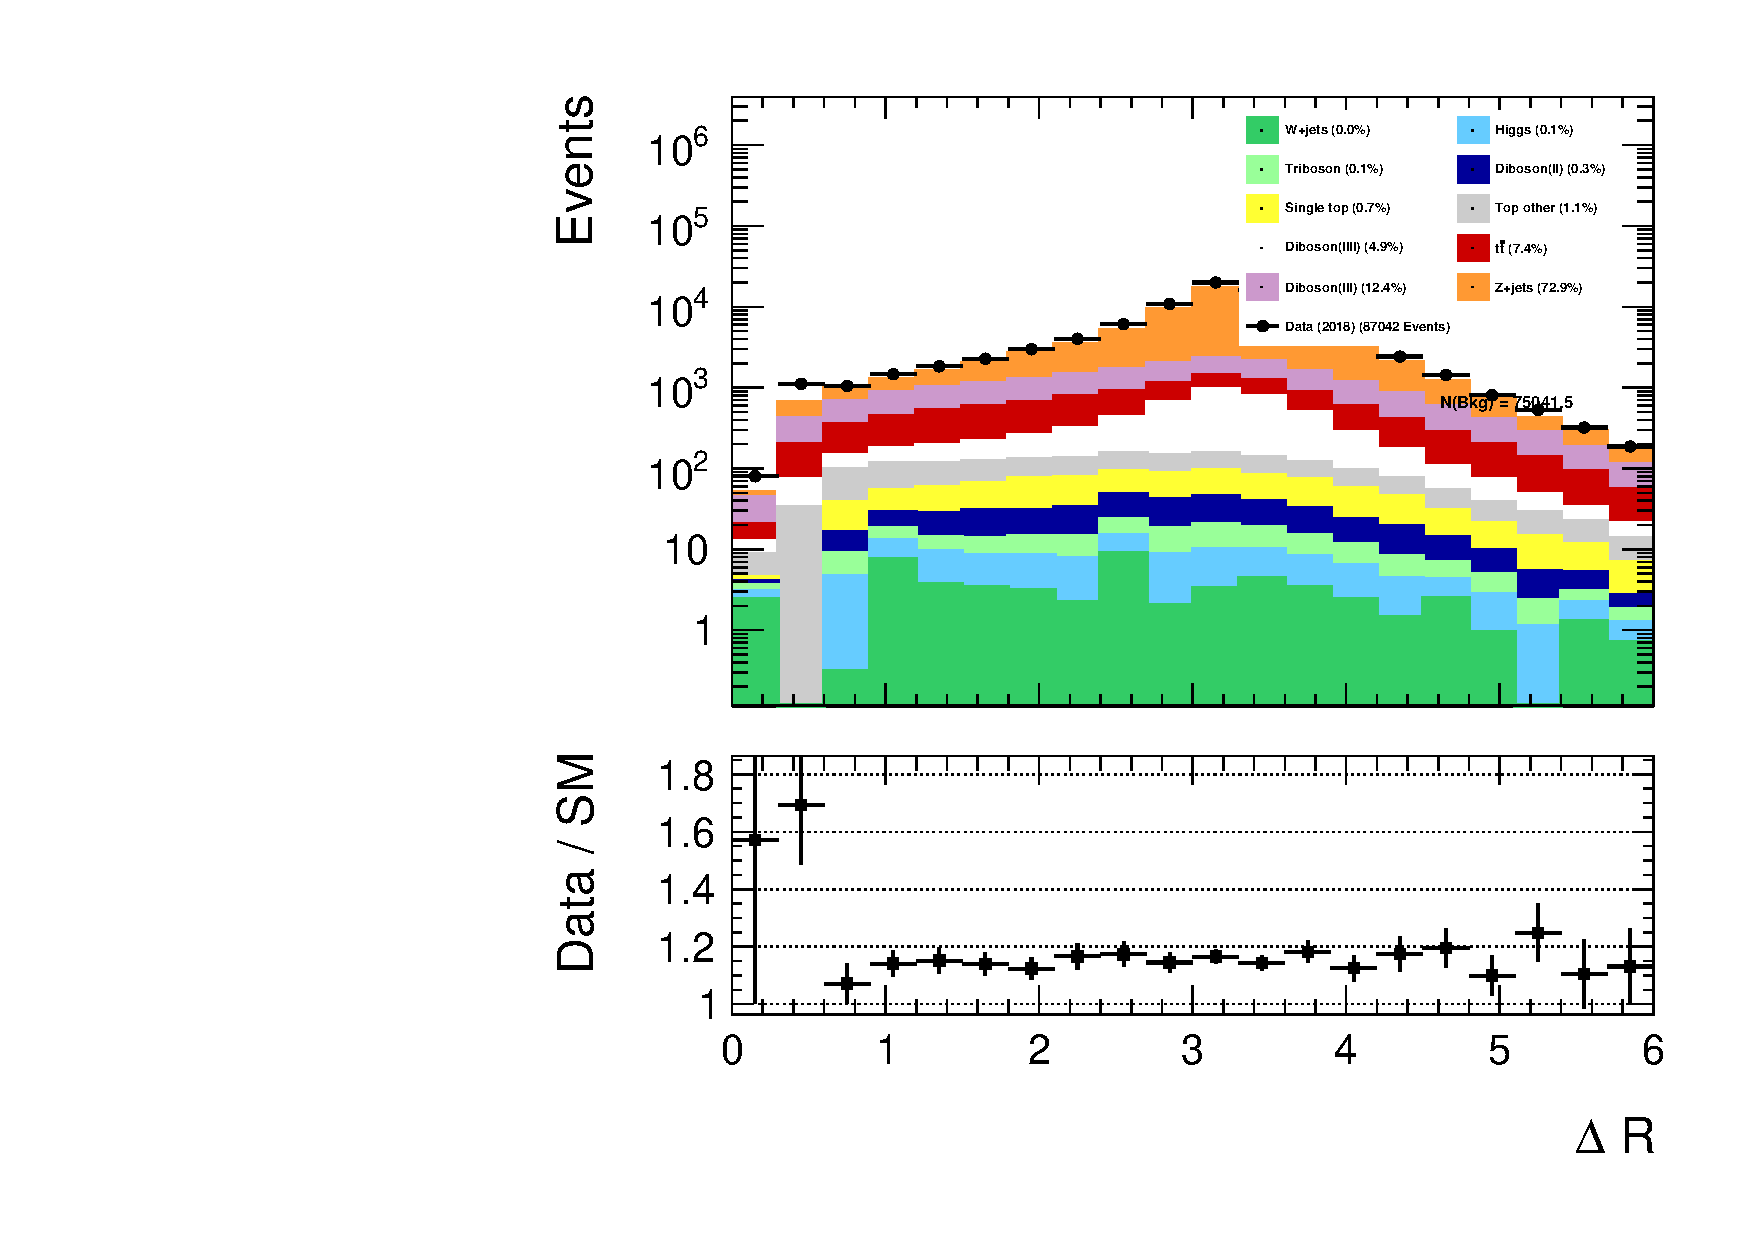
\includegraphics[width=\textwidth]{Figures/FeaturesHistograms/deltaR.pdf}
        \caption{}
        \label{fig:deltaR}
    \end{subfigure}
    \hfill
    \begin{subfigure}{.425\textwidth}
        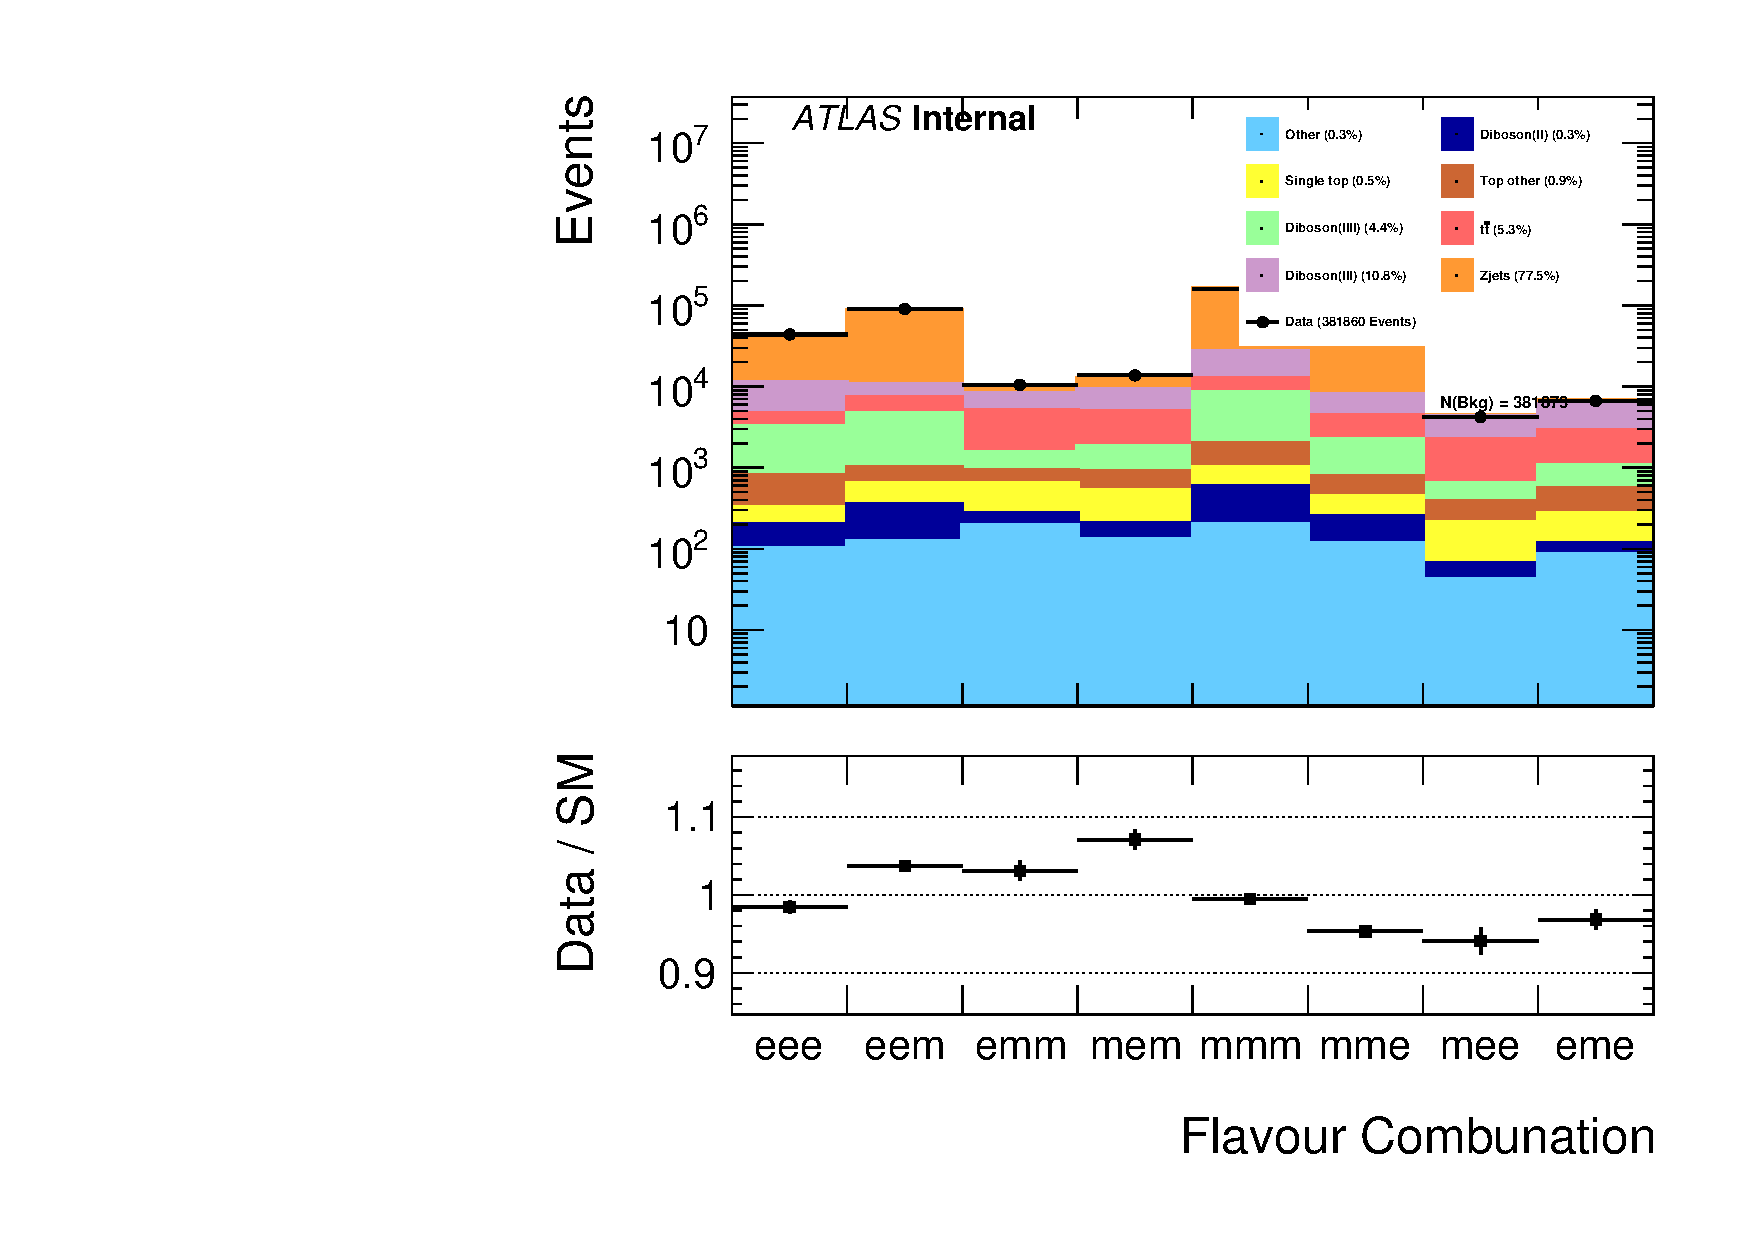
\includegraphics[width=\textwidth]{Figures/FeaturesHistograms/flcomp.pdf}
        \caption{}
        \label{fig:flcomp}
    \end{subfigure}
    }
    \makebox[0.9\linewidth][c]{%
    \begin{subfigure}{.425\textwidth}
        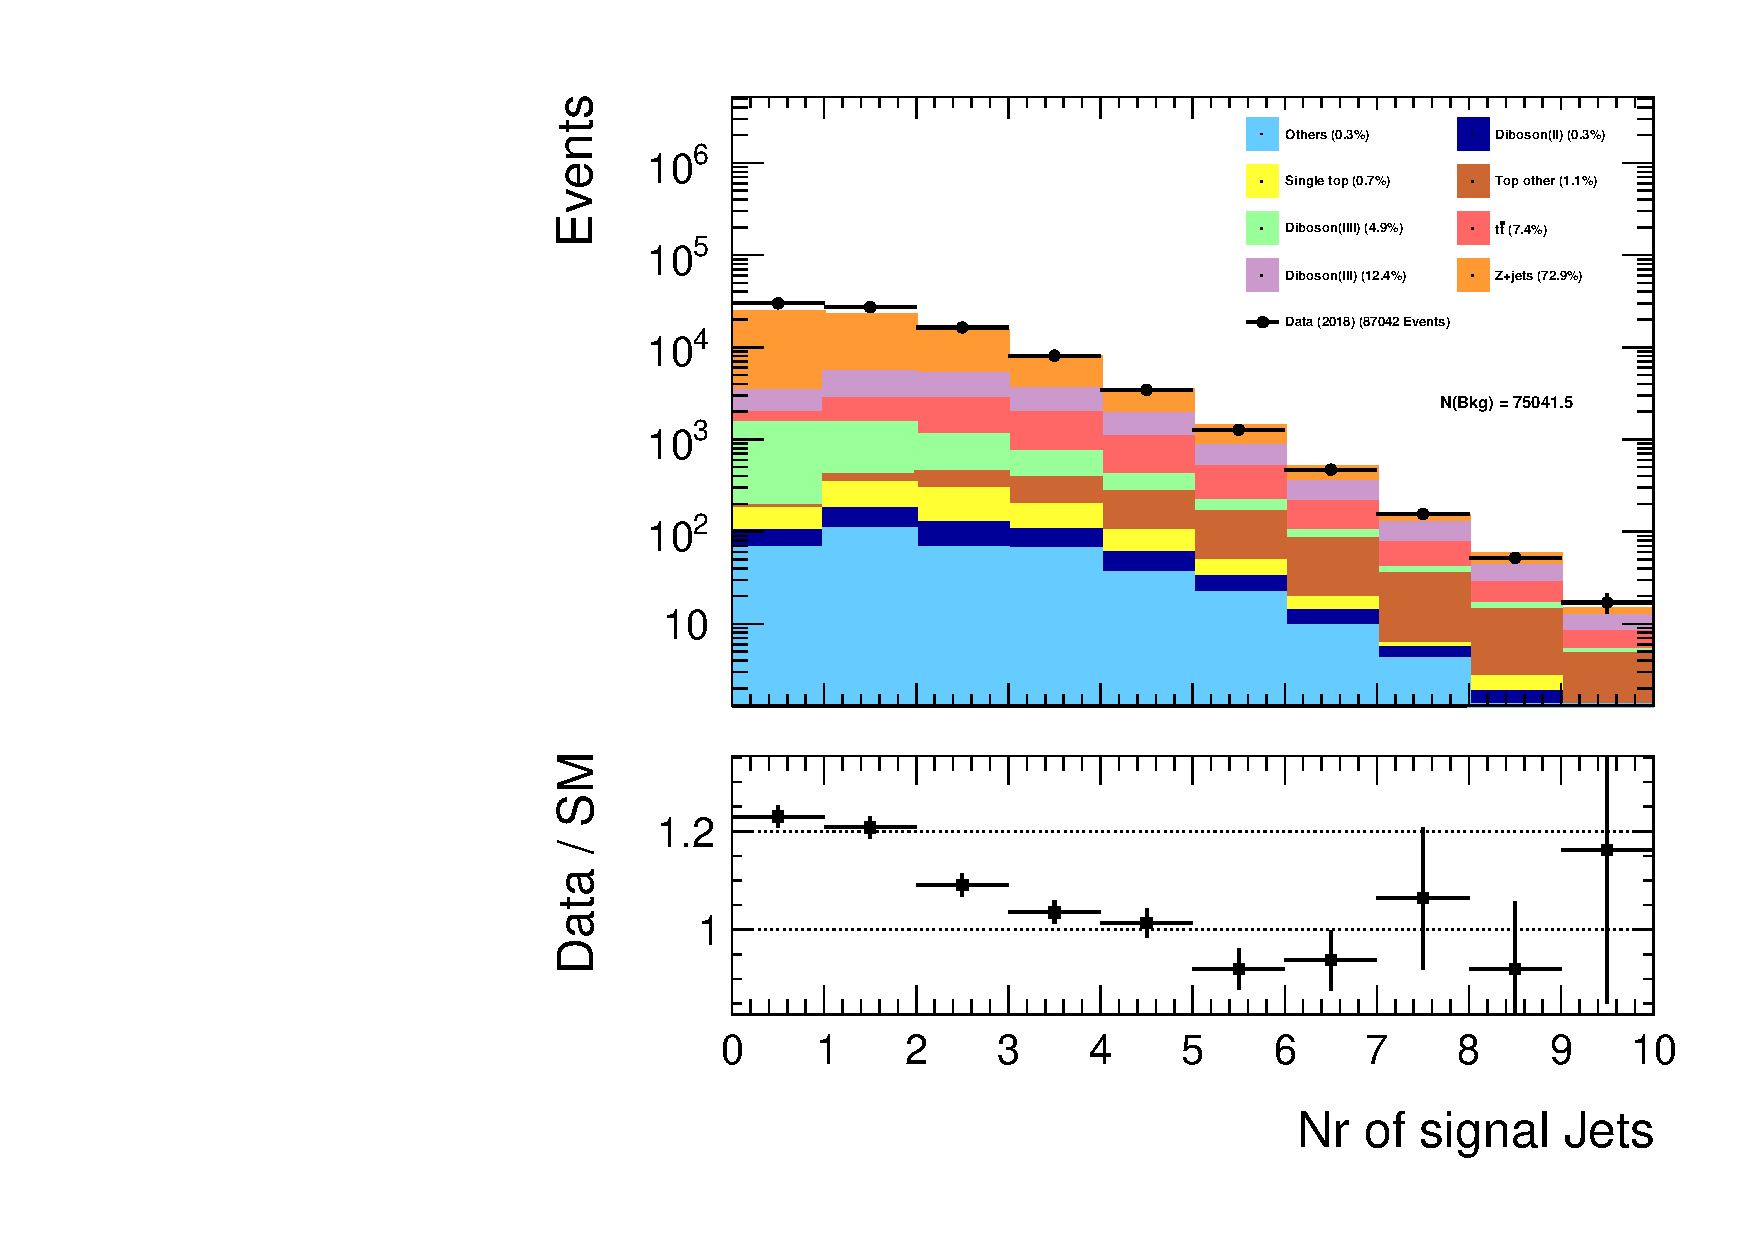
\includegraphics[width=\textwidth]{Figures/FeaturesHistograms/njet_SG.pdf}
        \caption{}
        \label{fig:njet_SG}
    \end{subfigure}
    \hfill
    \begin{subfigure}{.425\textwidth}
        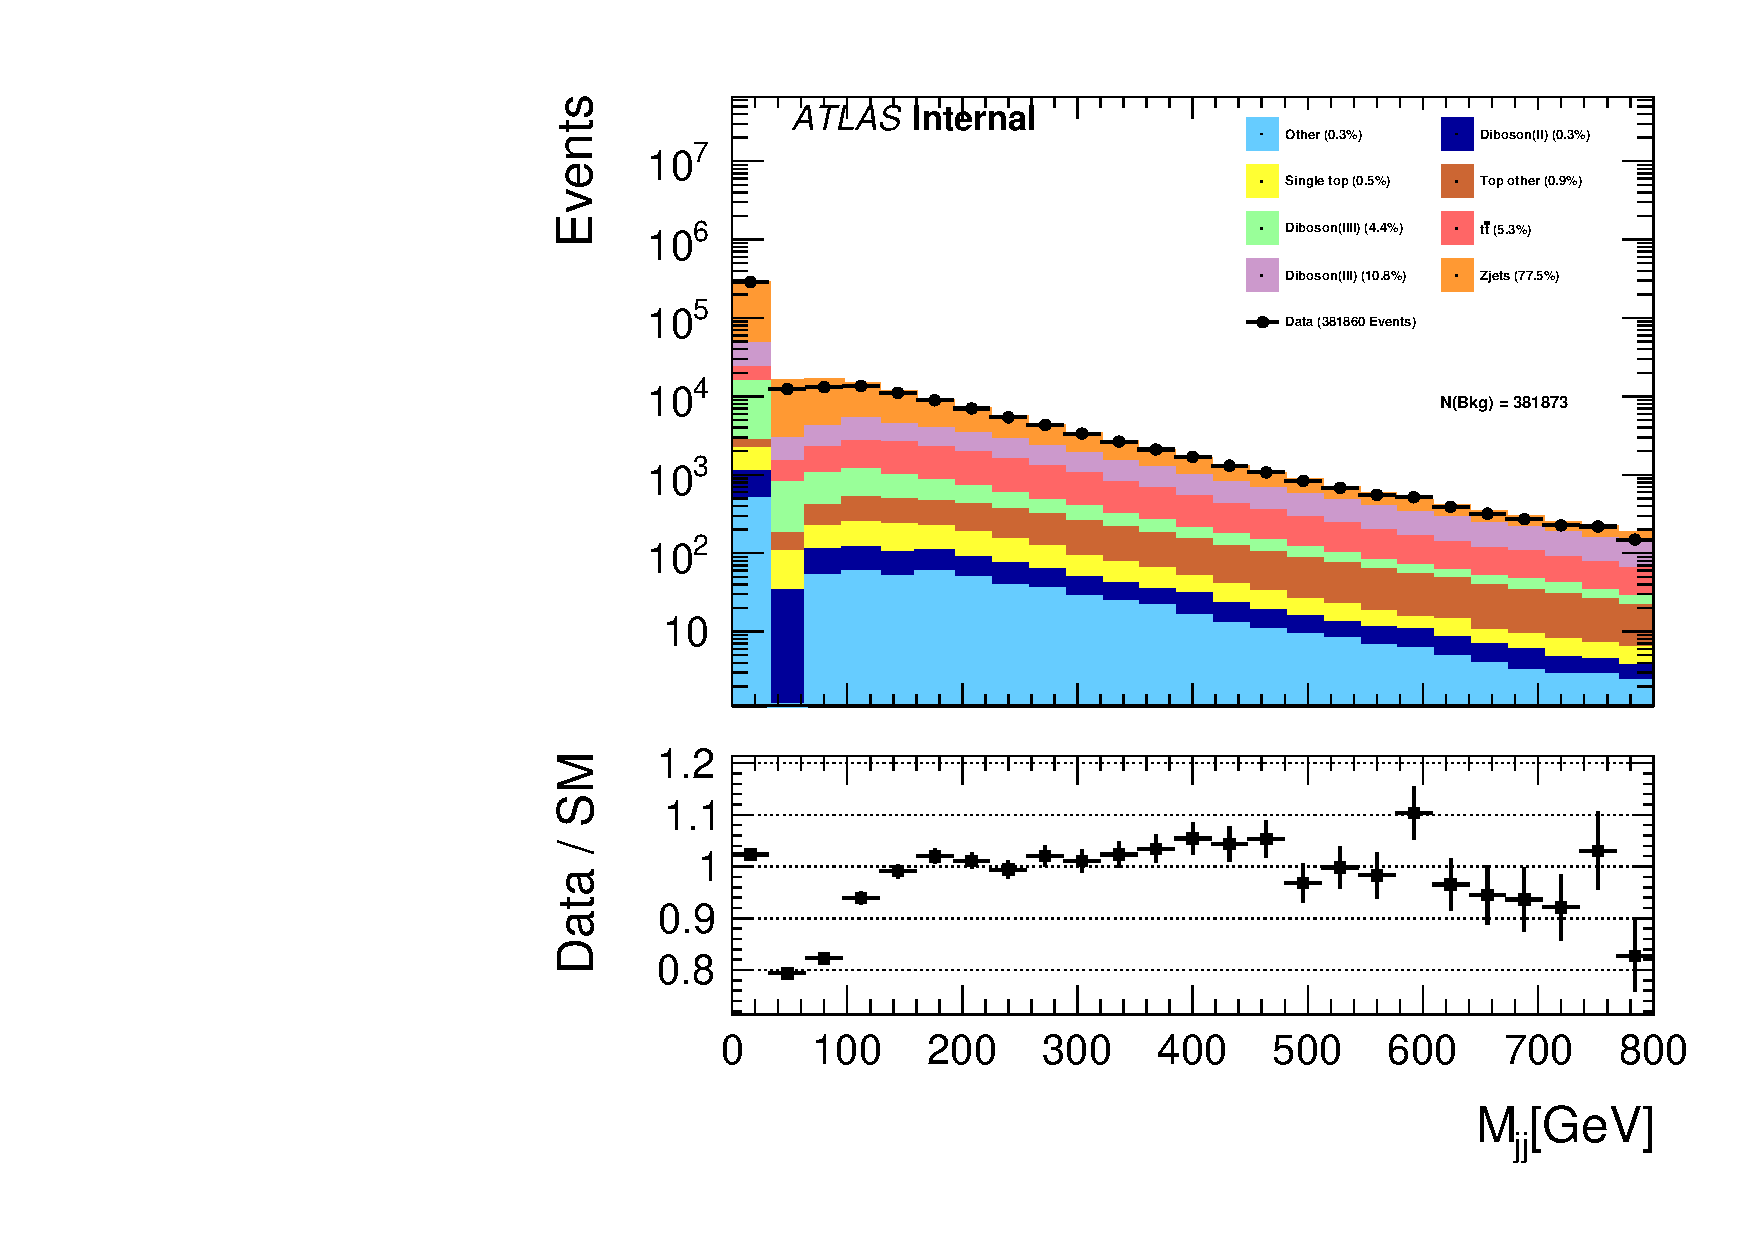
\includegraphics[width=\textwidth]{Figures/FeaturesHistograms/M_jj.pdf}
        \caption{}
        \label{fig:M_jj}
    \end{subfigure}
    }
    \caption{The event distribution for each channel over the sum of $P_t$
    for the SS pair \ref{fig:Ht_SS} and the sum over all three leptons added with $E_t^{miss}$
    \ref{fig:Ht_met_Et}. The distribution over $\Delta R$ \ref{fig:deltaR} and the flavor 
    combination of the three leptons \ref{fig:flcomp}. The distribution of number of jets 
    \ref{fig:njet_SG} and the mass of the leading di-jet pair \ref{fig:M_jj}.}
\end{figure}
\newpage
\begin{figure}
    \makebox[0.9\linewidth][c]{%
    \centering
    \begin{subfigure}{.425\textwidth}
        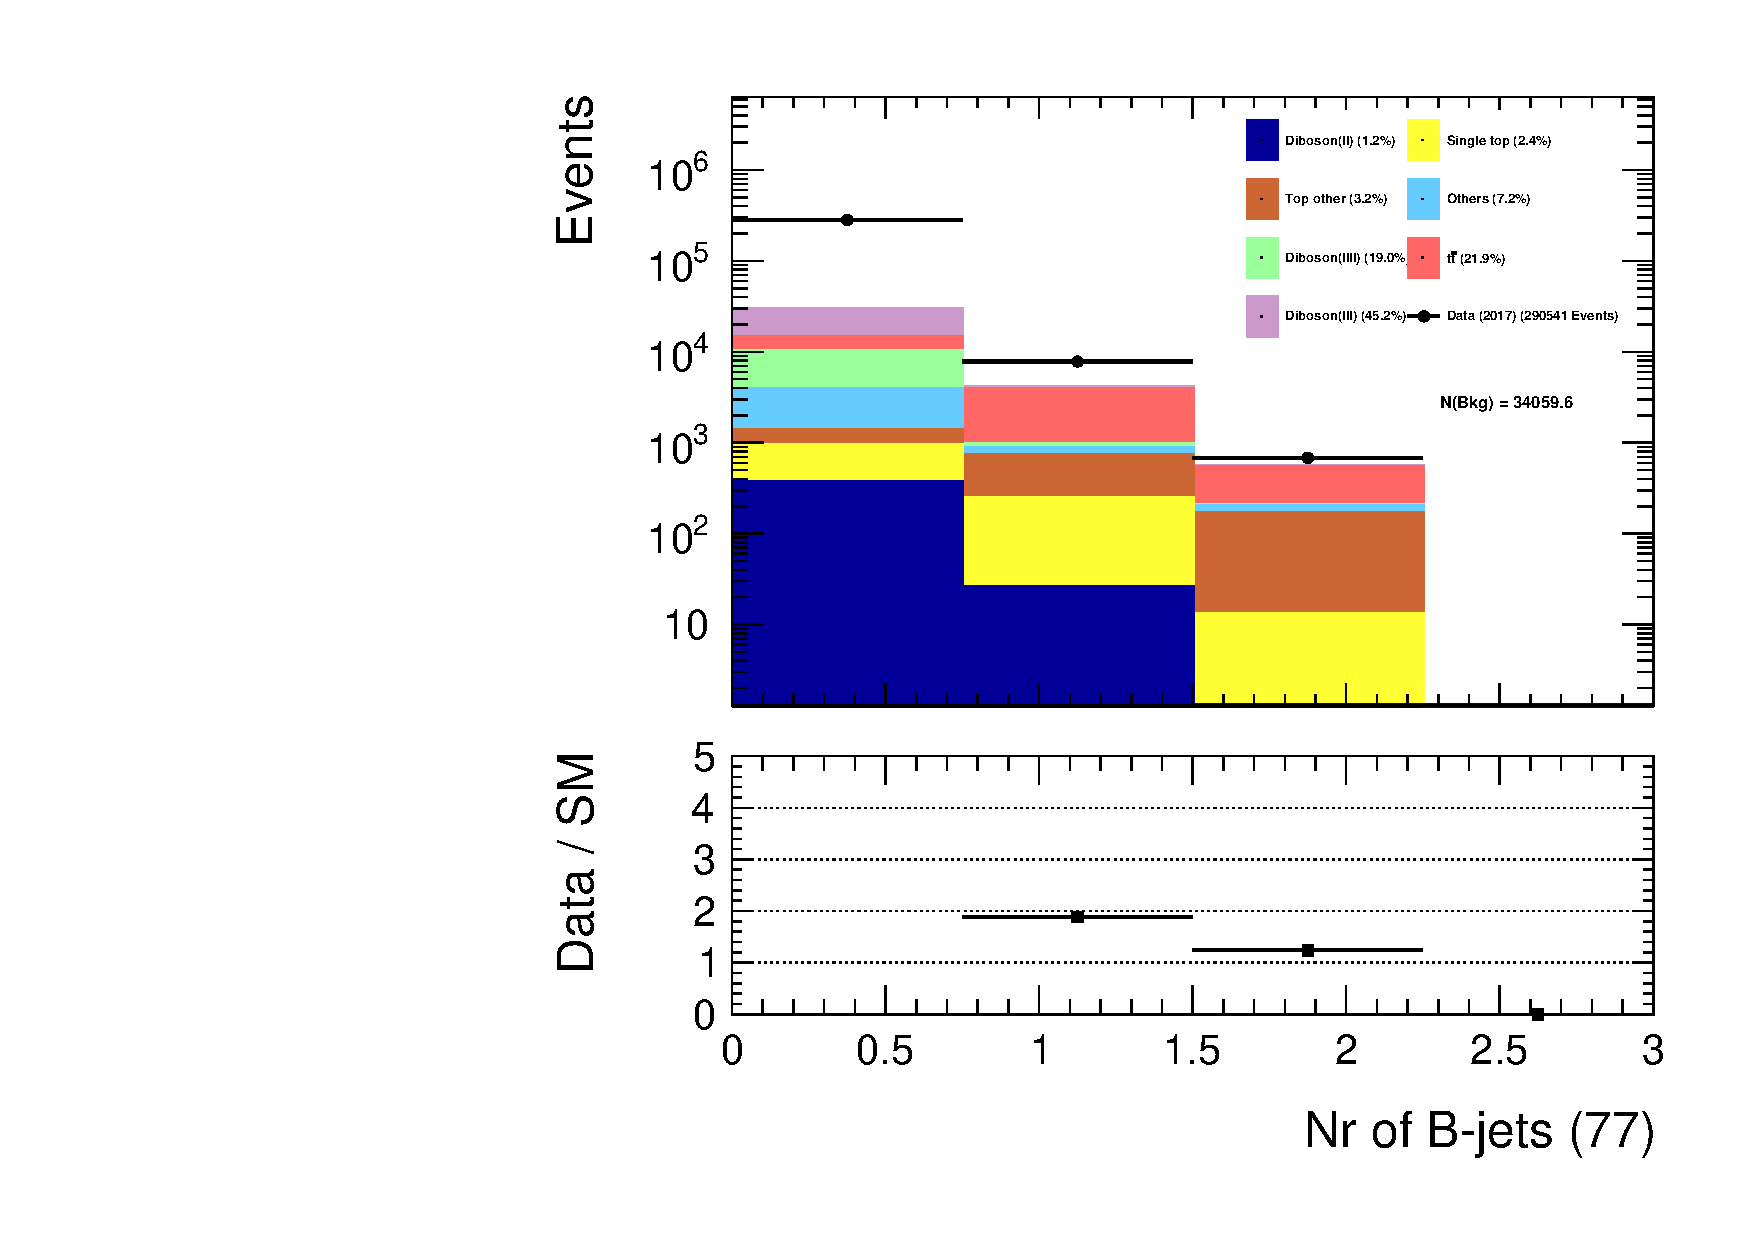
\includegraphics[width=\textwidth]{Figures/FeaturesHistograms/nbjet77.pdf}
        \caption{}
        \label{fig:nbjet77}
    \end{subfigure}
    \hfill
    \begin{subfigure}{.425\textwidth}
        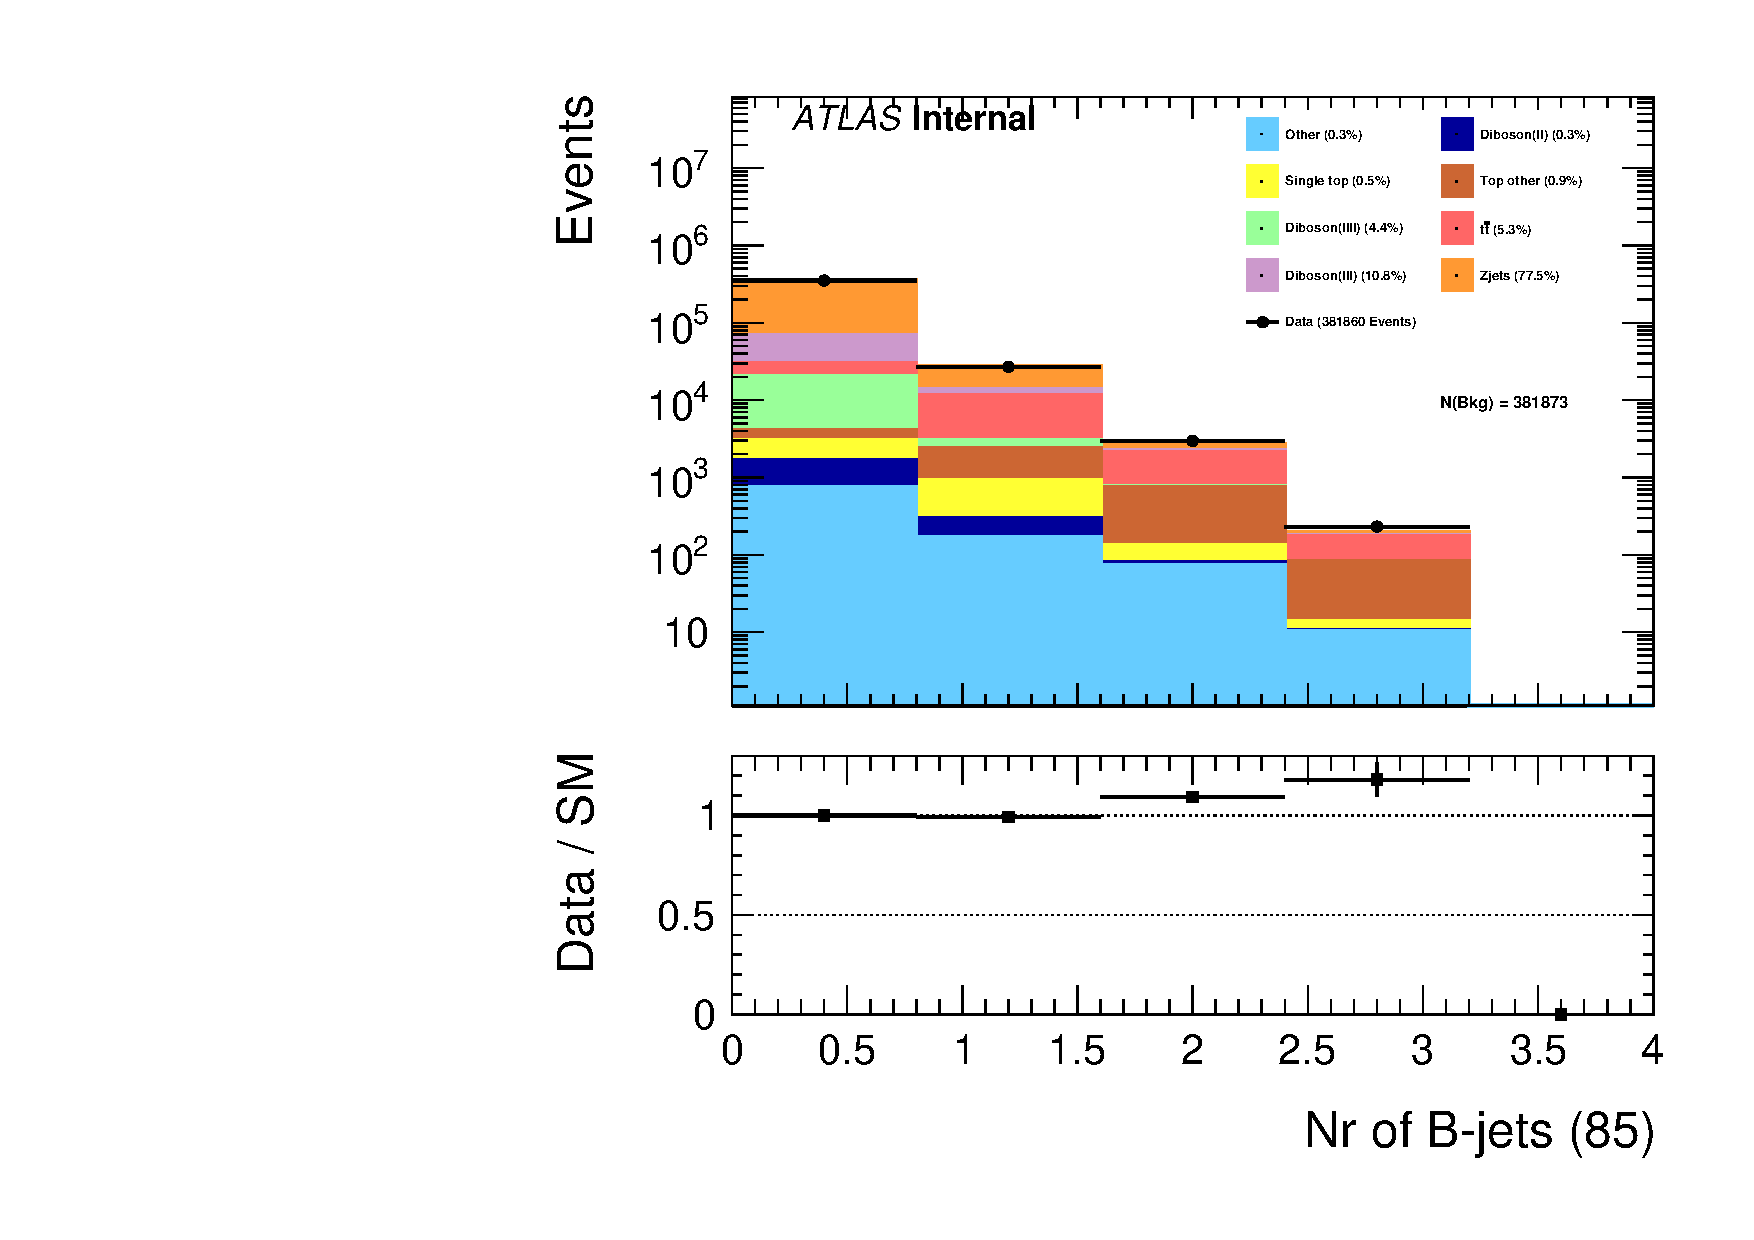
\includegraphics[width=\textwidth]{Figures/FeaturesHistograms/nbjet85.pdf}
        \caption{}
        \label{fig:nbjet85}
    \end{subfigure}
    }
    \caption{The event distribution for each channel over the number of b-jets 
    with $77\%$ \ref{fig:nbjet77} and $85\%$ \ref{fig:nbjet85} efficiency.}
    \label{fig:DistLast}
\end{figure}